%\pdfoutput=1
% Uncomment line above if submitting to arXiv and using pdflatex

% $Id: main.tex 33041 2013-03-25 16:12:53Z tgershon $
% ============================================================================
% Purpose: Template for LHCb documents
% Authors: Tomasz Skwarnicki, Roger Forty, Ulrik Egede
% Created on: 2010-09-24
% ============================================================================
\documentclass[12pt,a4paper]{article}
% For two column text, add "twocolumn" as an option to the document
% class. Also uncomment the two "onecolumn" and "twocolumn" lines
% around the title page below.

% Variables that controls behaviour
\usepackage{ifthen} % for conditional statements
\newboolean{pdflatex}
\setboolean{pdflatex}{true} % False for eps figures 

\newboolean{articletitles}
\setboolean{articletitles}{true} % False removes titles in references

\newboolean{uprightparticles}
\setboolean{uprightparticles}{false} %True for upright particle symbols

\newboolean{inbibliography}
\setboolean{inbibliography}{false} %True once you enter the bibliography

% THis file contains all the default packages and modifications for
% LHCb formatting

%% %%%%%%%%%%%%%%%%%%
%%  Page formatting
%% %%%%%%%%%%%%%%%%%%
\textheight=230mm
\textwidth=160mm
\oddsidemargin=7mm
\evensidemargin=-10mm
\topmargin=-10mm
\headsep=20mm
\columnsep=5mm
\addtolength{\belowcaptionskip}{0.5em}

\renewcommand{\textfraction}{0.01}
\renewcommand{\floatpagefraction}{0.99}
\renewcommand{\topfraction}{0.9}
\renewcommand{\bottomfraction}{0.9}


\setlength{\hoffset}{-2cm}
\setlength{\voffset}{-2cm}
% Page defaults ...
\topmargin=0.5cm
\oddsidemargin=2.5cm
\textwidth=16cm
\textheight=22cm
% Allow the page size to vary a bit ...
\raggedbottom
% To avoid Latex to be too fussy with line breaking ...
\sloppy

%% %%%%%%%%%%%%%%%%%%%%%%%
%% Packages to be used
%% %%%%%%%%%%%%%%%%%%%%%%% 
\usepackage{microtype}
\usepackage{lineno}  % for line numbering during review
\usepackage{xspace} % To avoid problems with missing or double spaces after
                    % predefined symbold


%% Graphics
\usepackage{graphicx}  % to include figures (can also use other packages)
\usepackage{color}
\usepackage{colortbl}
\graphicspath{{./figs/}} % Make Latex search fig subdir for figures

%% Math
\usepackage{amsmath} % Adds a large collection of math symbols
\usepackage{amssymb}
\usepackage{amsfonts}
\usepackage{upgreek} % Adds in support for greek letters in roman typeset

%% fix to allow peaceful coexistence of line numbering and
%% mathematical objects
%% http://www.latex-community.org/forum/viewtopic.php?f=5&t=163
%%
\newcommand*\patchAmsMathEnvironmentForLineno[1]{%
\expandafter\let\csname old#1\expandafter\endcsname\csname #1\endcsname
\expandafter\let\csname oldend#1\expandafter\endcsname\csname
end#1\endcsname
 \renewenvironment{#1}%
   {\linenomath\csname old#1\endcsname}%
   {\csname oldend#1\endcsname\endlinenomath}%
}
\newcommand*\patchBothAmsMathEnvironmentsForLineno[1]{%
  \patchAmsMathEnvironmentForLineno{#1}%
  \patchAmsMathEnvironmentForLineno{#1*}%
}
\AtBeginDocument{%
\patchBothAmsMathEnvironmentsForLineno{equation}%
\patchBothAmsMathEnvironmentsForLineno{align}%
\patchBothAmsMathEnvironmentsForLineno{flalign}%
\patchBothAmsMathEnvironmentsForLineno{alignat}%
\patchBothAmsMathEnvironmentsForLineno{gather}%
\patchBothAmsMathEnvironmentsForLineno{multline}%
}

% Get hyperlinks to captions and in references.
% These do not work with revtex. Use "hypertext" as class option instead.
\usepackage{hyperref}    % Hyperlinks in references
\usepackage[all]{hypcap} % Internal hyperlinks to floats.

%%% $Id: lhcb-symbols-def.tex 37234 2013-06-12 08:52:11Z roldeman $
%%% ======================================================================
%%% Purpose: Standard LHCb aliases
%%% Author: Originally Ulrik Egede, adapted by Tomasz Skwarnicki for templates,
%%% rewritten by Chris Parkes
%%% Maintainer : Ulrik Egede (2010 - 2012)
%%% =======================================================================

%%% To use this file outside the normal LHCb document environment, the
%%% following should be added in a preamble (before \begin{document}
%%%
%%%\usepackage{ifthen} 
%%%\newboolean{uprightparticles}
%%%\setboolean{uprightparticles}{false} %Set true for upright particle symbols
%%% \usepackage{xspace} 
%%% \usepackage{upgreek}

%%%%%%%%%%%%%%%%%%%%%%%%%%%%%%%%%%%%%%%%%%%%%%%%%%%%%%%%%%%%
%%%
%%% The following is to ensure that the template automatically can process
%%% this file.
%%%
%%% Add comments with at least three %%% preceding.
%%% Add new sections with one % preceding
%%% Add new subsections with two %% preceding
%%%%%%%%%%%%%%%%%%%%%%%%%%%%%%%%%%%%%%%%%%%%%%%%%%%%%%%%%%%%

%%%%%%%%%%%%%
% Experiments
%%%%%%%%%%%%%
\def\lhcb {\mbox{LHCb}\xspace}
\def\atlas  {\mbox{ATLAS}\xspace}
\def\cms    {\mbox{CMS}\xspace}
\def\alice  {\mbox{ALICE}\xspace}
\def\babar  {\mbox{BaBar}\xspace}
\def\belle  {\mbox{Belle}\xspace}
\def\cleo   {\mbox{CLEO}\xspace}
\def\cdf    {\mbox{CDF}\xspace}
\def\dzero  {\mbox{D0}\xspace}
\def\aleph  {\mbox{ALEPH}\xspace}
\def\delphi {\mbox{DELPHI}\xspace}
\def\opal   {\mbox{OPAL}\xspace}
\def\lthree {\mbox{L3}\xspace}
\def\sld    {\mbox{SLD}\xspace}
%%%\def\argus  {\mbox{ARGUS}\xspace}
%%%\def\uaone  {\mbox{UA1}\xspace}
%%%\def\uatwo  {\mbox{UA2}\xspace}
%%%\def\ux85 {\mbox{UX85}\xspace}
\def\cern {\mbox{CERN}\xspace}
\def\lhc    {\mbox{LHC}\xspace}
\def\lep    {\mbox{LEP}\xspace}
\def\tevatron {Tevatron\xspace}

%% LHCb sub-detectors and sub-systems

%%%\def\pu     {PU\xspace}
\def\velo   {VELO\xspace}
\def\rich   {RICH\xspace}
\def\richone {RICH1\xspace}
\def\richtwo {RICH2\xspace}
\def\ttracker {TT\xspace}
\def\intr   {IT\xspace}
\def\st     {ST\xspace}
\def\ot     {OT\xspace}
%%%\def\Tone   {T1\xspace}
%%%\def\Ttwo   {T2\xspace}
%%%\def\Tthree {T3\xspace}
%%%\def\Mone   {M1\xspace}
%%%\def\Mtwo   {M2\xspace}
%%%\def\Mthree {M3\xspace}
%%%\def\Mfour  {M4\xspace}
%%%\def\Mfive  {M5\xspace}
\def\spd    {SPD\xspace}
\def\presh  {PS\xspace}
\def\ecal   {ECAL\xspace}
\def\hcal   {HCAL\xspace}
%%%\def\bcm    {BCM\xspace}

%%%\def\ode    {ODE\xspace}
%%%\def\daq    {DAQ\xspace}
%%%\def\tfc    {TFC\xspace}
%%%\def\ecs    {ECS\xspace}
%%%\def\lone   {L0\xspace}
%%%\def\hlt    {HLT\xspace}
%%%\def\hltone {HLT1\xspace}
%%%\def\hlttwo {HLT2\xspace}

%%% Upright (not slanted) Particles

\ifthenelse{\boolean{uprightparticles}}%
{\def\Palpha      {\ensuremath{\upalpha}\xspace}
 \def\Pbeta       {\ensuremath{\upbeta}\xspace}
 \def\Pgamma      {\ensuremath{\upgamma}\xspace}                 
 \def\Pdelta      {\ensuremath{\updelta}\xspace}                 
 \def\Pepsilon    {\ensuremath{\upepsilon}\xspace}                 
 \def\Pvarepsilon {\ensuremath{\upvarepsilon}\xspace}                 
 \def\Pzeta       {\ensuremath{\upzeta}\xspace}                 
 \def\Peta        {\ensuremath{\upeta}\xspace}                 
 \def\Ptheta      {\ensuremath{\uptheta}\xspace}                 
 \def\Pvartheta   {\ensuremath{\upvartheta}\xspace}                 
 \def\Piota       {\ensuremath{\upiota}\xspace}                 
 \def\Pkappa      {\ensuremath{\upkappa}\xspace}                 
 \def\Plambda     {\ensuremath{\uplambda}\xspace}                 
 \def\Pmu         {\ensuremath{\upmu}\xspace}                 
 \def\Pnu         {\ensuremath{\upnu}\xspace}                 
 \def\Pxi         {\ensuremath{\upxi}\xspace}                 
 \def\Ppi         {\ensuremath{\uppi}\xspace}                 
 \def\Pvarpi      {\ensuremath{\upvarpi}\xspace}                 
 \def\Prho        {\ensuremath{\uprho}\xspace}                 
 \def\Pvarrho     {\ensuremath{\upvarrho}\xspace}                 
 \def\Ptau        {\ensuremath{\uptau}\xspace}                 
 \def\Pupsilon    {\ensuremath{\upupsilon}\xspace}                 
 \def\Pphi        {\ensuremath{\upphi}\xspace}                 
 \def\Pvarphi     {\ensuremath{\upvarphi}\xspace}                 
 \def\Pchi        {\ensuremath{\upchi}\xspace}                 
 \def\Ppsi        {\ensuremath{\uppsi}\xspace}                 
 \def\Pomega      {\ensuremath{\upomega}\xspace}                 

 \def\PDelta      {\ensuremath{\Delta}\xspace}                 
 \def\PXi      {\ensuremath{\Xi}\xspace}                 
 \def\PLambda      {\ensuremath{\Lambda}\xspace}                 
 \def\PSigma      {\ensuremath{\Sigma}\xspace}                 
 \def\POmega      {\ensuremath{\Omega}\xspace}                 
 \def\PUpsilon      {\ensuremath{\Upsilon}\xspace}                 
 
 %\mathchardef\Deltares="7101
 %\mathchardef\Xi="7104
 %\mathchardef\Lambda="7103
 %\mathchardef\Sigma="7106
 %\mathchardef\Omega="710A


 \def\PA      {\ensuremath{\mathrm{A}}\xspace}                 
 \def\PB      {\ensuremath{\mathrm{B}}\xspace}                 
 \def\PC      {\ensuremath{\mathrm{C}}\xspace}                 
 \def\PD      {\ensuremath{\mathrm{D}}\xspace}                 
 \def\PE      {\ensuremath{\mathrm{E}}\xspace}                 
 \def\PF      {\ensuremath{\mathrm{F}}\xspace}                 
 \def\PG      {\ensuremath{\mathrm{G}}\xspace}                 
 \def\PH      {\ensuremath{\mathrm{H}}\xspace}                 
 \def\PI      {\ensuremath{\mathrm{I}}\xspace}                 
 \def\PJ      {\ensuremath{\mathrm{J}}\xspace}                 
 \def\PK      {\ensuremath{\mathrm{K}}\xspace}                 
 \def\PL      {\ensuremath{\mathrm{L}}\xspace}                 
 \def\PM      {\ensuremath{\mathrm{M}}\xspace}                 
 \def\PN      {\ensuremath{\mathrm{N}}\xspace}                 
 \def\PO      {\ensuremath{\mathrm{O}}\xspace}                 
 \def\PP      {\ensuremath{\mathrm{P}}\xspace}                 
 \def\PQ      {\ensuremath{\mathrm{Q}}\xspace}                 
 \def\PR      {\ensuremath{\mathrm{R}}\xspace}                 
 \def\PS      {\ensuremath{\mathrm{S}}\xspace}                 
 \def\PT      {\ensuremath{\mathrm{T}}\xspace}                 
 \def\PU      {\ensuremath{\mathrm{U}}\xspace}                 
 \def\PV      {\ensuremath{\mathrm{V}}\xspace}                 
 \def\PW      {\ensuremath{\mathrm{W}}\xspace}                 
 \def\PX      {\ensuremath{\mathrm{X}}\xspace}                 
 \def\PY      {\ensuremath{\mathrm{Y}}\xspace}                 
 \def\PZ      {\ensuremath{\mathrm{Z}}\xspace}                 
 \def\Pa      {\ensuremath{\mathrm{a}}\xspace}                 
 \def\Pb      {\ensuremath{\mathrm{b}}\xspace}                 
 \def\Pc      {\ensuremath{\mathrm{c}}\xspace}                 
 \def\Pd      {\ensuremath{\mathrm{d}}\xspace}                 
 \def\Pe      {\ensuremath{\mathrm{e}}\xspace}                 
 \def\Pf      {\ensuremath{\mathrm{f}}\xspace}                 
 \def\Pg      {\ensuremath{\mathrm{g}}\xspace}                 
 \def\Ph      {\ensuremath{\mathrm{h}}\xspace}                 
 \def\Pi      {\ensuremath{\mathrm{i}}\xspace}                 
 \def\Pj      {\ensuremath{\mathrm{j}}\xspace}                 
 \def\Pk      {\ensuremath{\mathrm{k}}\xspace}                 
 \def\Pl      {\ensuremath{\mathrm{l}}\xspace}                 
 \def\Pm      {\ensuremath{\mathrm{m}}\xspace}                 
 \def\Pn      {\ensuremath{\mathrm{n}}\xspace}                 
 \def\Po      {\ensuremath{\mathrm{o}}\xspace}                 
 \def\Pp      {\ensuremath{\mathrm{p}}\xspace}                 
 \def\Pq      {\ensuremath{\mathrm{q}}\xspace}                 
 \def\Pr      {\ensuremath{\mathrm{r}}\xspace}                 
 \def\Ps      {\ensuremath{\mathrm{s}}\xspace}                 
 \def\Pt      {\ensuremath{\mathrm{t}}\xspace}                 
 \def\Pu      {\ensuremath{\mathrm{u}}\xspace}                 
 \def\Pv      {\ensuremath{\mathrm{v}}\xspace}                 
 \def\Pw      {\ensuremath{\mathrm{w}}\xspace}                 
 \def\Px      {\ensuremath{\mathrm{x}}\xspace}                 
 \def\Py      {\ensuremath{\mathrm{y}}\xspace}                 
 \def\Pz      {\ensuremath{\mathrm{z}}\xspace}                 
}
{\def\Palpha      {\ensuremath{\alpha}\xspace}
 \def\Pbeta       {\ensuremath{\beta}\xspace}
 \def\Pgamma      {\ensuremath{\gamma}\xspace}                 
 \def\Pdelta      {\ensuremath{\delta}\xspace}                 
 \def\Pepsilon    {\ensuremath{\epsilon}\xspace}                 
 \def\Pvarepsilon {\ensuremath{\varepsilon}\xspace}                 
 \def\Pzeta       {\ensuremath{\zeta}\xspace}                 
 \def\Peta        {\ensuremath{\eta}\xspace}                 
 \def\Ptheta      {\ensuremath{\theta}\xspace}                 
 \def\Pvartheta   {\ensuremath{\vartheta}\xspace}                 
 \def\Piota       {\ensuremath{\iota}\xspace}                 
 \def\Pkappa      {\ensuremath{\kappa}\xspace}                 
 \def\Plambda     {\ensuremath{\lambda}\xspace}                 
 \def\Pmu         {\ensuremath{\mu}\xspace}                 
 \def\Pnu         {\ensuremath{\nu}\xspace}                 
 \def\Pxi         {\ensuremath{\xi}\xspace}                 
 \def\Ppi         {\ensuremath{\pi}\xspace}                 
 \def\Pvarpi      {\ensuremath{\varpi}\xspace}                 
 \def\Prho        {\ensuremath{\rho}\xspace}                 
 \def\Pvarrho     {\ensuremath{\varrho}\xspace}                 
 \def\Ptau        {\ensuremath{\tau}\xspace}                 
 \def\Pupsilon    {\ensuremath{\upsilon}\xspace}                 
 \def\Pphi        {\ensuremath{\phi}\xspace}                 
 \def\Pvarphi     {\ensuremath{\varphi}\xspace}                 
 \def\Pchi        {\ensuremath{\chi}\xspace}                 
 \def\Ppsi        {\ensuremath{\psi}\xspace}                 
 \def\Pomega      {\ensuremath{\omega}\xspace}                 
 \mathchardef\PDelta="7101
 \mathchardef\PXi="7104
 \mathchardef\PLambda="7103
 \mathchardef\PSigma="7106
 \mathchardef\POmega="710A
 \mathchardef\PUpsilon="7107
 \def\PA      {\ensuremath{A}\xspace}                 
 \def\PB      {\ensuremath{B}\xspace}                 
 \def\PC      {\ensuremath{C}\xspace}                 
 \def\PD      {\ensuremath{D}\xspace}                 
 \def\PE      {\ensuremath{E}\xspace}                 
 \def\PF      {\ensuremath{F}\xspace}                 
 \def\PG      {\ensuremath{G}\xspace}                 
 \def\PH      {\ensuremath{H}\xspace}                 
 \def\PI      {\ensuremath{I}\xspace}                 
 \def\PJ      {\ensuremath{J}\xspace}                 
 \def\PK      {\ensuremath{K}\xspace}                 
 \def\PL      {\ensuremath{L}\xspace}                 
 \def\PM      {\ensuremath{M}\xspace}                 
 \def\PN      {\ensuremath{N}\xspace}                 
 \def\PO      {\ensuremath{O}\xspace}                 
 \def\PP      {\ensuremath{P}\xspace}                 
 \def\PQ      {\ensuremath{Q}\xspace}                 
 \def\PR      {\ensuremath{R}\xspace}                 
 \def\PS      {\ensuremath{S}\xspace}                 
 \def\PT      {\ensuremath{T}\xspace}                 
 \def\PU      {\ensuremath{U}\xspace}                 
 \def\PV      {\ensuremath{V}\xspace}                 
 \def\PW      {\ensuremath{W}\xspace}                 
 \def\PX      {\ensuremath{X}\xspace}                 
 \def\PY      {\ensuremath{Y}\xspace}                 
 \def\PZ      {\ensuremath{Z}\xspace}                 
 \def\Pa      {\ensuremath{a}\xspace}                 
 \def\Pb      {\ensuremath{b}\xspace}                 
 \def\Pc      {\ensuremath{c}\xspace}                 
 \def\Pd      {\ensuremath{d}\xspace}                 
 \def\Pe      {\ensuremath{e}\xspace}                 
 \def\Pf      {\ensuremath{f}\xspace}                 
 \def\Pg      {\ensuremath{g}\xspace}                 
 \def\Ph      {\ensuremath{h}\xspace}                 
 \def\Pi      {\ensuremath{i}\xspace}                 
 \def\Pj      {\ensuremath{j}\xspace}                 
 \def\Pk      {\ensuremath{k}\xspace}                 
 \def\Pl      {\ensuremath{l}\xspace}                 
 \def\Pm      {\ensuremath{m}\xspace}                 
 \def\Pn      {\ensuremath{n}\xspace}                 
 \def\Po      {\ensuremath{o}\xspace}                 
 \def\Pp      {\ensuremath{p}\xspace}                 
 \def\Pq      {\ensuremath{q}\xspace}                 
 \def\Pr      {\ensuremath{r}\xspace}                 
 \def\Ps      {\ensuremath{s}\xspace}                 
 \def\Pt      {\ensuremath{t}\xspace}                 
 \def\Pu      {\ensuremath{u}\xspace}                 
 \def\Pv      {\ensuremath{v}\xspace}                 
 \def\Pw      {\ensuremath{w}\xspace}                 
 \def\Px      {\ensuremath{x}\xspace}                 
 \def\Py      {\ensuremath{y}\xspace}                 
 \def\Pz      {\ensuremath{z}\xspace}                 
}

%%%%%%%%%%%%%%%%%%%%%%%%%%%%%%%%%%%%%%%%%%%%%%%
% Particles

%% Leptons

\let\emi\en
\def\electron   {\ensuremath{\Pe}\xspace}
\def\en         {\ensuremath{\Pe^-}\xspace}   % electron negative (\em is taken)
\def\ep         {\ensuremath{\Pe^+}\xspace}
\def\epm        {\ensuremath{\Pe^\pm}\xspace} 
\def\epem       {\ensuremath{\Pe^+\Pe^-}\xspace}
%%%\def\ee         {\ensuremath{\Pe^-\Pe^-}\xspace}

\def\mmu        {\ensuremath{\Pmu}\xspace}
\def\mup        {\ensuremath{\Pmu^+}\xspace}
\def\mun        {\ensuremath{\Pmu^-}\xspace} % muon negative (\mum is taken)
\def\mumu       {\ensuremath{\Pmu^+\Pmu^-}\xspace}
\def\mtau       {\ensuremath{\Ptau}\xspace}

\def\taup       {\ensuremath{\Ptau^+}\xspace}
\def\taum       {\ensuremath{\Ptau^-}\xspace}
\def\tautau     {\ensuremath{\Ptau^+\Ptau^-}\xspace}

\def\ellm       {\ensuremath{\ell^-}\xspace}
\def\ellp       {\ensuremath{\ell^+}\xspace}
%%%\def\ellell     {\ensuremath{\ell^+ \ell^-}\xspace}

\def\neu        {\ensuremath{\Pnu}\xspace}
\def\neub       {\ensuremath{\overline{\Pnu}}\xspace}
%%%\def\nuenueb    {\ensuremath{\neu\neub}\xspace}
\def\neue       {\ensuremath{\neu_e}\xspace}
\def\neueb      {\ensuremath{\neub_e}\xspace}
%%%\def\neueneueb  {\ensuremath{\neue\neueb}\xspace}
\def\neum       {\ensuremath{\neu_\mu}\xspace}
\def\neumb      {\ensuremath{\neub_\mu}\xspace}
%%%\def\neumneumb  {\ensuremath{\neum\neumb}\xspace}
\def\neut       {\ensuremath{\neu_\tau}\xspace}
\def\neutb      {\ensuremath{\neub_\tau}\xspace}
%%%\def\neutneutb  {\ensuremath{\neut\neutb}\xspace}
\def\neul       {\ensuremath{\neu_\ell}\xspace}
\def\neulb      {\ensuremath{\neub_\ell}\xspace}
%%%\def\neulneulb  {\ensuremath{\neul\neulb}\xspace}

%% Gauge bosons and scalars

\def\g      {\ensuremath{\Pgamma}\xspace}
\def\H      {\ensuremath{\PH^0}\xspace}
\def\Hp     {\ensuremath{\PH^+}\xspace}
\def\Hm     {\ensuremath{\PH^-}\xspace}
\def\Hpm    {\ensuremath{\PH^\pm}\xspace}
\def\W      {\ensuremath{\PW}\xspace}
\def\Wp     {\ensuremath{\PW^+}\xspace}
\def\Wm     {\ensuremath{\PW^-}\xspace}
\def\Wpm    {\ensuremath{\PW^\pm}\xspace}
\def\Z      {\ensuremath{\PZ}\xspace}

%% Quarks

\def\quark     {\ensuremath{\Pq}\xspace}
\def\quarkbar  {\ensuremath{\overline \quark}\xspace}
\def\qqbar     {\ensuremath{\quark\quarkbar}\xspace}
\def\uquark    {\ensuremath{\Pu}\xspace}
\def\uquarkbar {\ensuremath{\overline \uquark}\xspace}
\def\uubar     {\ensuremath{\uquark\uquarkbar}\xspace}
\def\dquark    {\ensuremath{\Pd}\xspace}
\def\dquarkbar {\ensuremath{\overline \dquark}\xspace}
\def\ddbar     {\ensuremath{\dquark\dquarkbar}\xspace}
\def\squark    {\ensuremath{\Ps}\xspace}
\def\squarkbar {\ensuremath{\overline \squark}\xspace}
\def\ssbar     {\ensuremath{\squark\squarkbar}\xspace}
\def\cquark    {\ensuremath{\Pc}\xspace}
\def\cquarkbar {\ensuremath{\overline \cquark}\xspace}
\def\ccbar     {\ensuremath{\cquark\cquarkbar}\xspace}
\def\bquark    {\ensuremath{\Pb}\xspace}
\def\bquarkbar {\ensuremath{\overline \bquark}\xspace}
\def\bbbar     {\ensuremath{\bquark\bquarkbar}\xspace}
\def\tquark    {\ensuremath{\Pt}\xspace}
\def\tquarkbar {\ensuremath{\overline \tquark}\xspace}
\def\ttbar     {\ensuremath{\tquark\tquarkbar}\xspace}

%% Light mesons

\def\pion  {\ensuremath{\Ppi}\xspace}
\def\piz   {\ensuremath{\pion^0}\xspace}
\def\pizs  {\ensuremath{\pion^0\mbox\,\rm{s}}\xspace}
%%%\def\ppz   {\ensuremath{\pion^0\pion^0}\xspace}
\def\pip   {\ensuremath{\pion^+}\xspace}
\def\pim   {\ensuremath{\pion^-}\xspace}
%%%\def\pipi  {\ensuremath{\pion^+\pion^-}\xspace}
\def\pipm  {\ensuremath{\pion^\pm}\xspace}
\def\pimp  {\ensuremath{\pion^\mp}\xspace}

\def\kaon  {\ensuremath{\PK}\xspace}
%%% do NOT use ensuremath here
  \def\Kbar  {\kern 0.2em\overline{\kern -0.2em \PK}{}\xspace}
\def\Kb    {\ensuremath{\Kbar}\xspace}
\def\Kz    {\ensuremath{\kaon^0}\xspace}
\def\Kzb   {\ensuremath{\Kbar^0}\xspace}
%%%\def\KzKzb {\ensuremath{\Kz \kern -0.16em \Kzb}\xspace}
\def\Kp    {\ensuremath{\kaon^+}\xspace}
\def\Km    {\ensuremath{\kaon^-}\xspace}
\def\Kpm   {\ensuremath{\kaon^\pm}\xspace}
\def\Kmp   {\ensuremath{\kaon^\mp}\xspace}
%%%\def\KpKm  {\ensuremath{\Kp \kern -0.16em \Km}\xspace}
\def\KS    {\ensuremath{\kaon^0_{\rm\scriptscriptstyle S}}\xspace} 
\def\KL    {\ensuremath{\kaon^0_{\rm\scriptscriptstyle L}}\xspace} 
\def\Kstarz  {\ensuremath{\kaon^{*0}}\xspace}
\def\Kstarzb {\ensuremath{\Kbar^{*0}}\xspace}
\def\Kstar   {\ensuremath{\kaon^*}\xspace}
\def\Kstarb  {\ensuremath{\Kbar^*}\xspace}
\def\Kstarp  {\ensuremath{\kaon^{*+}}\xspace}
\def\Kstarm  {\ensuremath{\kaon^{*-}}\xspace}
\def\Kstarpm {\ensuremath{\kaon^{*\pm}}\xspace}
\def\Kstarmp {\ensuremath{\kaon^{*\mp}}\xspace}

\newcommand{\etapr}{\ensuremath{\Peta^{\prime}}\xspace}

%% Heavy mesons

%%% do NOT use ensuremath here
  \def\Dbar    {\kern 0.2em\overline{\kern -0.2em \PD}{}\xspace}
\def\D       {\ensuremath{\PD}\xspace}
\def\Db      {\ensuremath{\Dbar}\xspace}
\def\Dz      {\ensuremath{\D^0}\xspace}
\def\Dzb     {\ensuremath{\Dbar^0}\xspace}
%%%\def\DzDzb   {\ensuremath{\Dz {\kern -0.16em \Dzb}}\xspace}
\def\Dp      {\ensuremath{\D^+}\xspace}
\def\Dm      {\ensuremath{\D^-}\xspace}
\def\Dpm     {\ensuremath{\D^\pm}\xspace}
\def\Dmp     {\ensuremath{\D^\mp}\xspace}
%%%\def\DpDm    {\ensuremath{\Dp {\kern -0.16em \Dm}}\xspace}
\def\Dstar   {\ensuremath{\D^*}\xspace}
\def\Dstarb  {\ensuremath{\Dbar^*}\xspace}
\def\Dstarz  {\ensuremath{\D^{*0}}\xspace}
\def\Dstarzb {\ensuremath{\Dbar^{*0}}\xspace}
\def\Dstarp  {\ensuremath{\D^{*+}}\xspace}
\def\Dstarm  {\ensuremath{\D^{*-}}\xspace}
\def\Dstarpm {\ensuremath{\D^{*\pm}}\xspace}
\def\Dstarmp {\ensuremath{\D^{*\mp}}\xspace}
\def\Ds      {\ensuremath{\D^+_\squark}\xspace}
\def\Dsp     {\ensuremath{\D^+_\squark}\xspace}
\def\Dsm     {\ensuremath{\D^-_\squark}\xspace}
\def\Dspm    {\ensuremath{\D^{\pm}_\squark}\xspace}
\def\Dsmp    {\ensuremath{\D^{\mp}_\squark}\xspace}
\def\Dss     {\ensuremath{\D^{*+}_\squark}\xspace}
\def\Dssp    {\ensuremath{\D^{*+}_\squark}\xspace}
\def\Dssm    {\ensuremath{\D^{*-}_\squark}\xspace}
\def\Dsspm   {\ensuremath{\D^{*\pm}_\squark}\xspace}
\def\Dssmp   {\ensuremath{\D^{*\mp}_\squark}\xspace}

\def\B       {\ensuremath{\PB}\xspace}
%%% do NOT use ensuremath here
\def\Bbar    {\ensuremath{\kern 0.18em\overline{\kern -0.18em \PB}{}}\xspace}
\def\Bb      {\ensuremath{\Bbar}\xspace}
%%%\def\BBbar   {\ensuremath{\B\Bbar}\xspace} 
\def\Bz      {\ensuremath{\B^0}\xspace}
\def\Bzb     {\ensuremath{\Bbar^0}\xspace}
\def\Bu      {\ensuremath{\B^+}\xspace}
\def\Bub     {\ensuremath{\B^-}\xspace}
\def\Bp      {\ensuremath{\Bu}\xspace}
\def\Bm      {\ensuremath{\Bub}\xspace}
\def\Bpm     {\ensuremath{\B^\pm}\xspace}
\def\Bmp     {\ensuremath{\B^\mp}\xspace}
\def\Bd      {\ensuremath{\B^0}\xspace}
\def\Bs      {\ensuremath{\B^0_\squark}\xspace}
\def\Bsb     {\ensuremath{\Bbar^0_\squark}\xspace}
\def\Bdb     {\ensuremath{\Bbar^0}\xspace}
\def\Bc      {\ensuremath{\B_\cquark^+}\xspace}
\def\Bcp     {\ensuremath{\B_\cquark^+}\xspace}
\def\Bcm     {\ensuremath{\B_\cquark^-}\xspace}
\def\Bcpm    {\ensuremath{\B_\cquark^\pm}\xspace}

%% Onia

\def\jpsi     {\ensuremath{{\PJ\mskip -3mu/\mskip -2mu\Ppsi\mskip 2mu}}\xspace}
\def\psitwos  {\ensuremath{\Ppsi{(2S)}}\xspace}
\def\psiprpr  {\ensuremath{\Ppsi(3770)}\xspace}
\def\etac     {\ensuremath{\Peta_\cquark}\xspace}
\def\chiczero {\ensuremath{\Pchi_{\cquark 0}}\xspace}
\def\chicone  {\ensuremath{\Pchi_{\cquark 1}}\xspace}
\def\chictwo  {\ensuremath{\Pchi_{\cquark 2}}\xspace}
  %\mathchardef\Upsilon="7107
  \def\Y#1S{\ensuremath{\PUpsilon{(#1S)}}\xspace}% no space before {...}!
\def\OneS  {\Y1S}
\def\TwoS  {\Y2S}
\def\ThreeS{\Y3S}
\def\FourS {\Y4S}
\def\FiveS {\Y5S}

\def\chic  {\ensuremath{\Pchi_{c}}\xspace}

\def\chib {\ensuremath{\Pchi_{\bquark}}\xspace}
\def\chibzero {\ensuremath{\Pchi_{\bquark 0}}\xspace}
\def\chibone  {\ensuremath{\Pchi_{\bquark 1}}\xspace}
\def\chibtwo  {\ensuremath{\Pchi_{\bquark 2}}\xspace}

\def\chibOneP  {\ensuremath{\Pchi_{\bquark}(1P)}\xspace}
\def\chibTwoP  {\ensuremath{\Pchi_{\bquark}(2P)}\xspace}
\def\chibThreeP  {\ensuremath{\Pchi_{\bquark}(3P)}\xspace}

\def\chiboneOneP  {\ensuremath{\Pchi_{\bquark 1}(1P)}\xspace}
\def\chiboneTwoP  {\ensuremath{\Pchi_{\bquark 1}(2P)}\xspace}
\def\chiboneThreeP  {\ensuremath{(\Pchi_{\bquark 1}3P)}\xspace}

\def\chibtwoOneP  {\ensuremath{\Pchi_{\bquark 2}(1P)}\xspace}
\def\chibtwoTwoP  {\ensuremath{\Pchi_{\bquark 2}(2P)}\xspace}
\def\chibtwoThreeP  {\ensuremath{\Pchi_{\bquark 2}(3P)}\xspace}



%% Baryons

\def\proton      {\ensuremath{\Pp}\xspace}
\def\antiproton  {\ensuremath{\overline \proton}\xspace}
\def\neutron     {\ensuremath{\Pn}\xspace}
\def\antineutron {\ensuremath{\overline \neutron}\xspace}

\def\Deltares {\ensuremath{\PDelta}\xspace}
\def\Deltaresbar{\ensuremath{\overline \Deltares}\xspace}
\def\Xires {\ensuremath{\PXi}\xspace}
\def\Xiresbar{\ensuremath{\overline \Xires}\xspace}
\def\Lz {\ensuremath{\PLambda}\xspace}
\def\Lbar {\ensuremath{\kern 0.1em\overline{\kern -0.1em\PLambda}}\xspace}
\def\Lambdares {\ensuremath{\PLambda}\xspace}
\def\Lambdaresbar{\ensuremath{\Lbar}\xspace}
\def\Sigmares {\ensuremath{\PSigma}\xspace}
\def\Sigmaresbar{\ensuremath{\overline \Sigmares}\xspace}
\def\Omegares {\ensuremath{\POmega^-}\xspace}
\def\Omegaresbar{\ensuremath{\overline{\POmega}^+}\xspace}

%%% do NOT use ensuremath here
 % \def\Deltabar{\kern 0.25em\overline{\kern -0.25em \Deltares}{}\xspace}
 % \def\Sigbar{\kern 0.2em\overline{\kern -0.2em \Sigma}{}\xspace}
 % \def\Xibar{\kern 0.2em\overline{\kern -0.2em \Xi}{}\xspace}
 % \def\Obar{\kern 0.2em\overline{\kern -0.2em \Omega}{}\xspace}
 % \def\Nbar{\kern 0.2em\overline{\kern -0.2em N}{}\xspace}
 % \def\Xb{\kern 0.2em\overline{\kern -0.2em X}{}\xspace}

\def\Lb      {\ensuremath{\Lz^0_\bquark}\xspace}
\def\Lbbar   {\ensuremath{\Lbar^0_\bquark}\xspace}
\def\Lc      {\ensuremath{\Lz^+_\cquark}\xspace}
\def\Lcbar   {\ensuremath{\Lbar^-_\cquark}\xspace}

%%%%%%%%%%%%%%%%%%
% Physics symbols
%%%%%%%%%%%%%%%%%

%% Decays
\def\BF         {{\ensuremath{\cal B}\xspace}}
\def\BRvis      {{\ensuremath{\BR_{\rm{vis}}}}}
\def\BR         {\BF}
\newcommand{\decay}[2]{\ensuremath{#1\!\to #2}\xspace}         % {\Pa}{\Pb \Pc}
\def\ra                 {\ensuremath{\rightarrow}\xspace}
\def\to                 {\ensuremath{\rightarrow}\xspace}

%% Lifetimes
\newcommand{\tauBs}{\ensuremath{\tau_{\Bs}}\xspace}
\newcommand{\tauBd}{\ensuremath{\tau_{\Bd}}\xspace}
\newcommand{\tauBz}{\ensuremath{\tau_{\Bz}}\xspace}
\newcommand{\tauBu}{\ensuremath{\tau_{\Bp}}\xspace}
\newcommand{\tauDp}{\ensuremath{\tau_{\Dp}}\xspace}
\newcommand{\tauDz}{\ensuremath{\tau_{\Dz}}\xspace}
\newcommand{\tauL}{\ensuremath{\tau_{\rm L}}\xspace}
\newcommand{\tauH}{\ensuremath{\tau_{\rm H}}\xspace}

%% Masses
\newcommand{\mBd}{\ensuremath{m_{\Bd}}\xspace}
\newcommand{\mBp}{\ensuremath{m_{\Bp}}\xspace}
\newcommand{\mBs}{\ensuremath{m_{\Bs}}\xspace}
\newcommand{\mBc}{\ensuremath{m_{\Bc}}\xspace}
\newcommand{\mLb}{\ensuremath{m_{\Lb}}\xspace}

%% EW theory, groups
\def\grpsuthree {\ensuremath{\mathrm{SU}(3)}\xspace}
\def\grpsutw    {\ensuremath{\mathrm{SU}(2)}\xspace}
\def\grpuone    {\ensuremath{\mathrm{U}(1)}\xspace}

\def\ssqtw {\ensuremath{\sin^{2}\!\theta_{\mathrm{W}}}\xspace}
\def\csqtw {\ensuremath{\cos^{2}\!\theta_{\mathrm{W}}}\xspace}
\def\stw   {\ensuremath{\sin\theta_{\mathrm{W}}}\xspace}
\def\ctw   {\ensuremath{\cos\theta_{\mathrm{W}}}\xspace}
\def\ssqtwef {\ensuremath{{\sin}^{2}\theta_{\mathrm{W}}^{\mathrm{eff}}}\xspace}
\def\csqtwef {\ensuremath{{\cos}^{2}\theta_{\mathrm{W}}^{\mathrm{eff}}}\xspace}
\def\stwef {\ensuremath{\sin\theta_{\mathrm{W}}^{\mathrm{eff}}}\xspace}
\def\ctwef {\ensuremath{\cos\theta_{\mathrm{W}}^{\mathrm{eff}}}\xspace}
\def\gv    {\ensuremath{g_{\mbox{\tiny V}}}\xspace}
\def\ga    {\ensuremath{g_{\mbox{\tiny A}}}\xspace}

\def\order   {\ensuremath{\mathcal{O}}\xspace}
\def\ordalph {\ensuremath{\mathcal{O}(\alpha)}\xspace}
\def\ordalsq {\ensuremath{\mathcal{O}(\alpha^{2})}\xspace}
\def\ordalcb {\ensuremath{\mathcal{O}(\alpha^{3})}\xspace}

%% QCD parameters
\newcommand{\as}{\ensuremath{\alpha_s}\xspace}
\newcommand{\MSb}{\ensuremath{\overline{\mathrm{MS}}}\xspace}
\newcommand{\lqcd}{\ensuremath{\Lambda_{\mathrm{QCD}}}\xspace}
\def\qsq       {\ensuremath{q^2}\xspace}

%% CKM, CP violation

\def\eps   {\ensuremath{\varepsilon}\xspace}
\def\epsK  {\ensuremath{\varepsilon_K}\xspace}
\def\epsB  {\ensuremath{\varepsilon_B}\xspace}
\def\epsp  {\ensuremath{\varepsilon^\prime_K}\xspace}

\def\CP                {\ensuremath{C\!P}\xspace}
\def\CPT               {\ensuremath{C\!PT}\xspace}

\def\rhobar {\ensuremath{\overline \rho}\xspace}
\def\etabar {\ensuremath{\overline \eta}\xspace}

\def\Vud  {\ensuremath{|V_{\uquark\dquark}|}\xspace}
\def\Vcd  {\ensuremath{|V_{\cquark\dquark}|}\xspace}
\def\Vtd  {\ensuremath{|V_{\tquark\dquark}|}\xspace}
\def\Vus  {\ensuremath{|V_{\uquark\squark}|}\xspace}
\def\Vcs  {\ensuremath{|V_{\cquark\squark}|}\xspace}
\def\Vts  {\ensuremath{|V_{\tquark\squark}|}\xspace}
\def\Vub  {\ensuremath{|V_{\uquark\bquark}|}\xspace}
\def\Vcb  {\ensuremath{|V_{\cquark\bquark}|}\xspace}
\def\Vtb  {\ensuremath{|V_{\tquark\bquark}|}\xspace}

%% Oscillations

\newcommand{\dm}{\ensuremath{\Delta m}\xspace}
\newcommand{\dms}{\ensuremath{\Delta m_{\squark}}\xspace}
\newcommand{\dmd}{\ensuremath{\Delta m_{\dquark}}\xspace}
\newcommand{\DG}{\ensuremath{\Delta\Gamma}\xspace}
\newcommand{\DGs}{\ensuremath{\Delta\Gamma_{\squark}}\xspace}
\newcommand{\DGd}{\ensuremath{\Delta\Gamma_{\dquark}}\xspace}
\newcommand{\Gs}{\ensuremath{\Gamma_{\squark}}\xspace}
\newcommand{\Gd}{\ensuremath{\Gamma_{\dquark}}\xspace}

\newcommand{\MBq}{\ensuremath{M_{\B_\quark}}\xspace}
\newcommand{\DGq}{\ensuremath{\Delta\Gamma_{\quark}}\xspace}
\newcommand{\Gq}{\ensuremath{\Gamma_{\quark}}\xspace}
\newcommand{\dmq}{\ensuremath{\Delta m_{\quark}}\xspace}
\newcommand{\GL}{\ensuremath{\Gamma_{\rm L}}\xspace}
\newcommand{\GH}{\ensuremath{\Gamma_{\rm H}}\xspace}

\newcommand{\DGsGs}{\ensuremath{\Delta\Gamma_{\squark}/\Gamma_{\squark}}\xspace}
\newcommand{\Delm}{\mbox{$\Delta m $}\xspace}
\newcommand{\ACP}{\ensuremath{{\cal A}^{\CP}}\xspace}
\newcommand{\Adir}{\ensuremath{{\cal A}^{\rm dir}}\xspace}
\newcommand{\Amix}{\ensuremath{{\cal A}^{\rm mix}}\xspace}
\newcommand{\ADelta}{\ensuremath{{\cal A}^\Delta}\xspace}
\newcommand{\phid}{\ensuremath{\phi_{\dquark}}\xspace}
\newcommand{\sinphid}{\ensuremath{\sin\!\phid}\xspace}
\newcommand{\phis}{\ensuremath{\phi_{\squark}}\xspace}
\newcommand{\betas}{\ensuremath{\beta_{\squark}}\xspace}
\newcommand{\sbetas}{\ensuremath{\sigma(\beta_{\squark})}\xspace}
\newcommand{\stbetas}{\ensuremath{\sigma(2\beta_{\squark})}\xspace}
\newcommand{\stphis}{\ensuremath{\sigma(\phi_{\squark})}\xspace}
\newcommand{\sinphis}{\ensuremath{\sin\!\phis}\xspace}

%% Tagging
\newcommand{\edet}{{\ensuremath{\varepsilon_{\rm det}}}\xspace}
\newcommand{\erec}{{\ensuremath{\varepsilon_{\rm rec/det}}}\xspace}
\newcommand{\esel}{{\ensuremath{\varepsilon_{\rm sel/rec}}}\xspace}
\newcommand{\etrg}{{\ensuremath{\varepsilon_{\rm trg/sel}}}\xspace}
\newcommand{\etot}{{\ensuremath{\varepsilon_{\rm tot}}}\xspace}

\newcommand{\mistag}{\ensuremath{\omega}\xspace}
\newcommand{\wcomb}{\ensuremath{\omega^{\rm comb}}\xspace}
\newcommand{\etag}{{\ensuremath{\varepsilon_{\rm tag}}}\xspace}
\newcommand{\etagcomb}{{\ensuremath{\varepsilon_{\rm tag}^{\rm comb}}}\xspace}
\newcommand{\effeff}{\ensuremath{\varepsilon_{\rm eff}}\xspace}
\newcommand{\effeffcomb}{\ensuremath{\varepsilon_{\rm eff}^{\rm comb}}\xspace}
\newcommand{\efftag}{{\ensuremath{\etag(1-2\omega)^2}}\xspace}
\newcommand{\effD}{{\ensuremath{\etag D^2}}\xspace}

\newcommand{\etagprompt}{{\ensuremath{\varepsilon_{\rm tag}^{\rm Pr}}}\xspace}
\newcommand{\etagLL}{{\ensuremath{\varepsilon_{\rm tag}^{\rm LL}}}\xspace}

%% Key decay channels

\def\BdToKstmm    {\decay{\Bd}{\Kstarz\mup\mun}}
\def\BdbToKstmm   {\decay{\Bdb}{\Kstarzb\mup\mun}}

\def\BsToJPsiPhi  {\decay{\Bs}{\jpsi\phi}}
\def\BdToJPsiKst  {\decay{\Bd}{\jpsi\Kstarz}}
\def\BdbToJPsiKst {\decay{\Bdb}{\jpsi\Kstarzb}}

\def\BsPhiGam     {\decay{\Bs}{\phi \g}}
\def\BdKstGam     {\decay{\Bd}{\Kstarz \g}}

\def\BTohh        {\decay{\B}{\Ph^+ \Ph'^-}}
\def\BdTopipi     {\decay{\Bd}{\pip\pim}}
\def\BdToKpi      {\decay{\Bd}{\Kp\pim}}
\def\BsToKK       {\decay{\Bs}{\Kp\Km}}
\def\BsTopiK      {\decay{\Bs}{\pip\Km}}

%% Rare decays
\def\BdKstee  {\decay{\Bd}{\Kstarz\epem}}
\def\BdbKstee {\decay{\Bdb}{\Kstarzb\epem}}
\def\bsll     {\decay{\bquark}{\squark \ell^+ \ell^-}}
\def\AFB      {\ensuremath{A_{\mathrm{FB}}}\xspace}
\def\FL       {\ensuremath{F_{\mathrm{L}}}\xspace}
\def\AT#1     {\ensuremath{A_{\mathrm{T}}^{#1}}\xspace}           % 2
\def\btosgam  {\decay{\bquark}{\squark \g}}
\def\btodgam  {\decay{\bquark}{\dquark \g}}
\def\Bsmm     {\decay{\Bs}{\mup\mun}}
\def\Bdmm     {\decay{\Bd}{\mup\mun}}
\def\ctl       {\ensuremath{\cos{\theta_\ell}}\xspace}
\def\ctk       {\ensuremath{\cos{\theta_K}}\xspace}

%% Wilson coefficients and operators
\def\C#1      {\ensuremath{\mathcal{C}_{#1}}\xspace}                       % 9
\def\Cp#1     {\ensuremath{\mathcal{C}_{#1}^{'}}\xspace}                    % 7
\def\Ceff#1   {\ensuremath{\mathcal{C}_{#1}^{\mathrm{(eff)}}}\xspace}        % 9  
\def\Cpeff#1  {\ensuremath{\mathcal{C}_{#1}^{'\mathrm{(eff)}}}\xspace}       % 7
\def\Ope#1    {\ensuremath{\mathcal{O}_{#1}}\xspace}                       % 2
\def\Opep#1   {\ensuremath{\mathcal{O}_{#1}^{'}}\xspace}                    % 7

%% Charm

\def\xprime     {\ensuremath{x^{\prime}}\xspace}
\def\yprime     {\ensuremath{y^{\prime}}\xspace}
\def\ycp        {\ensuremath{y_{\CP}}\xspace}
\def\agamma     {\ensuremath{A_{\Gamma}}\xspace}
%%%\def\kpi        {\ensuremath{\PK\Ppi}\xspace}
%%%\def\kk         {\ensuremath{\PK\PK}\xspace}
%%%\def\dkpi       {\decay{\PD}{\PK\Ppi}}
%%%\def\dkk        {\decay{\PD}{\PK\PK}}
\def\dkpicf     {\decay{\Dz}{\Km\pip}}

%% QM
\newcommand{\bra}[1]{\ensuremath{\langle #1|}}             % {a}
\newcommand{\ket}[1]{\ensuremath{|#1\rangle}}              % {b}
\newcommand{\braket}[2]{\ensuremath{\langle #1|#2\rangle}} % {a}{b}

%%%%%%%%%%%%%%%%%%%%%%%%%%%%%%%%%%%%%%%%%%%%%%%%%%
% Units
%%%%%%%%%%%%%%%%%%%%%%%%%%%%%%%%%%%%%%%%%%%%%%%%%%
\newcommand{\unit}[1]{\ensuremath{\rm\,#1}\xspace}          % {kg}

%% Energy and momentum
\newcommand{\tev}{\ifthenelse{\boolean{inbibliography}}{\ensuremath{~T\kern -0.05em eV}\xspace}{\ensuremath{\mathrm{\,Te\kern -0.1em V}}\xspace}}
\newcommand{\gev}{\ensuremath{\mathrm{\,Ge\kern -0.1em V}}\xspace}
\newcommand{\mev}{\ensuremath{\mathrm{\,Me\kern -0.1em V}}\xspace}
\newcommand{\kev}{\ensuremath{\mathrm{\,ke\kern -0.1em V}}\xspace}
\newcommand{\ev}{\ensuremath{\mathrm{\,e\kern -0.1em V}}\xspace}
\newcommand{\gevc}{\ensuremath{{\mathrm{\,Ge\kern -0.1em V\!/}c}}\xspace}
\newcommand{\mevc}{\ensuremath{{\mathrm{\,Me\kern -0.1em V\!/}c}}\xspace}
\newcommand{\gevcc}{\ensuremath{{\mathrm{\,Ge\kern -0.1em V\!/}c^2}}\xspace}
\newcommand{\gevgevcccc}{\ensuremath{{\mathrm{\,Ge\kern -0.1em V^2\!/}c^4}}\xspace}
\newcommand{\mevcc}{\ensuremath{{\mathrm{\,Me\kern -0.1em V\!/}c^2}}\xspace}

%% Distance and area
\def\km   {\ensuremath{\rm \,km}\xspace}
\def\m    {\ensuremath{\rm \,m}\xspace}
\def\cm   {\ensuremath{\rm \,cm}\xspace}
\def\cma  {\ensuremath{{\rm \,cm}^2}\xspace}
\def\mm   {\ensuremath{\rm \,mm}\xspace}
\def\mma  {\ensuremath{{\rm \,mm}^2}\xspace}
\def\mum  {\ensuremath{\,\upmu\rm m}\xspace}
\def\muma {\ensuremath{\,\upmu\rm m^2}\xspace}
\def\nm   {\ensuremath{\rm \,nm}\xspace}
\def\fm   {\ensuremath{\rm \,fm}\xspace}
\def\barn{\ensuremath{\rm \,b}\xspace}
%%%\def\barnhyph{\ensuremath{\rm -b}\xspace}
\def\mbarn{\ensuremath{\rm \,mb}\xspace}
\def\mub{\ensuremath{\rm \,\upmu b}\xspace}
%%%\def\mbarnhyph{\ensuremath{\rm -mb}\xspace}
\def\nb {\ensuremath{\rm \,nb}\xspace}
\def\invnb {\ensuremath{\mbox{\,nb}^{-1}}\xspace}
\def\pb {\ensuremath{\rm \,pb}\xspace}
\def\invpb {\ensuremath{\mbox{\,pb}^{-1}}\xspace}
\def\fb   {\ensuremath{\mbox{\,fb}}\xspace}
\def\invfb   {\ensuremath{\mbox{\,fb}^{-1}}\xspace}

%% Time 
\def\sec  {\ensuremath{\rm {\,s}}\xspace}
\def\ms   {\ensuremath{{\rm \,ms}}\xspace}
\def\mus  {\ensuremath{\,\upmu{\rm s}}\xspace}
\def\ns   {\ensuremath{{\rm \,ns}}\xspace}
\def\ps   {\ensuremath{{\rm \,ps}}\xspace}
\def\fs   {\ensuremath{\rm \,fs}\xspace}

\def\mhz  {\ensuremath{{\rm \,MHz}}\xspace}
\def\khz  {\ensuremath{{\rm \,kHz}}\xspace}
\def\hz   {\ensuremath{{\rm \,Hz}}\xspace}

\def\invps{\ensuremath{{\rm \,ps^{-1}}}\xspace}

\def\yr   {\ensuremath{\rm \,yr}\xspace}
\def\hr   {\ensuremath{\rm \,hr}\xspace}

%% Temperature
\def\degc {\ensuremath{^\circ}{C}\xspace}
\def\degk {\ensuremath {\rm K}\xspace}

%% Material lengths, radiation
\def\Xrad {\ensuremath{X_0}\xspace}
\def\NIL{\ensuremath{\lambda_{int}}\xspace}
\def\mip {MIP\xspace}
\def\neutroneq {\ensuremath{\rm \,n_{eq}}\xspace}
\def\neqcmcm {\ensuremath{\rm \,n_{eq} / cm^2}\xspace}
\def\kRad {\ensuremath{\rm \,kRad}\xspace}
\def\MRad {\ensuremath{\rm \,MRad}\xspace}
\def\ci {\ensuremath{\rm \,Ci}\xspace}
\def\mci {\ensuremath{\rm \,mCi}\xspace}

%% Uncertainties
\def\sx    {\ensuremath{\sigma_x}\xspace}    
\def\sy    {\ensuremath{\sigma_y}\xspace}   
\def\sz    {\ensuremath{\sigma_z}\xspace}    

\newcommand{\stat}{\ensuremath{\mathrm{\,(stat)}}\xspace}
\newcommand{\syst}{\ensuremath{\mathrm{\,(syst)}}\xspace}

%% Maths

\def\order{{\ensuremath{\cal O}}\xspace}
\newcommand{\chisq}{\ensuremath{\chi^2}\xspace}
\newcommand{\chisqndf}{\ensuremath{\chi^2/\mathrm{ndf}}\xspace}
\newcommand{\chisqip}{\ensuremath{\chi^2_{\rm IP}}\xspace}
\newcommand{\chisqvs}{\ensuremath{\chi^2_{\rm VS}}\xspace}
\newcommand{\chisqvtx}{\ensuremath{\chi^2_{\rm vtx}}\xspace}

\def\deriv {\ensuremath{\mathrm{d}}}

\def\gsim{{~\raise.15em\hbox{$>$}\kern-.85em
          \lower.35em\hbox{$\sim$}~}\xspace}
\def\lsim{{~\raise.15em\hbox{$<$}\kern-.85em
          \lower.35em\hbox{$\sim$}~}\xspace}

\newcommand{\mean}[1]{\ensuremath{\left\langle #1 \right\rangle}} % {x}
\newcommand{\abs}[1]{\ensuremath{\left\|#1\right\|}} % {x}
\newcommand{\Real}{\ensuremath{\mathcal{R}e}\xspace}
\newcommand{\Imag}{\ensuremath{\mathcal{I}m}\xspace}

\def\PDF {PDF\xspace}

\def\sPlot{\mbox{\em sPlot}}
\def\sWeight{\mbox{\em sWeight}}
%%%%%%%%%%%%%%%%%%%%%%%%%%%%%%%%%%%%%%%%%%%%%%%%%%
% Kinematics
%%%%%%%%%%%%%%%%%%%%%%%%%%%%%%%%%%%%%%%%%%%%%%%%%%

%% Energy, Momenta
\def\Ebeam {\ensuremath{E_{\mbox{\tiny BEAM}}}\xspace}
\def\sqs   {\ensuremath{\protect\sqrt{s}}\xspace}

\def\ptot       {\mbox{$p$}\xspace}
\def\pt         {\mbox{$p_{\rm T}$}\xspace}
\def\et         {\mbox{$E_{\rm T}$}\xspace}
\def\mt         {\mbox{$M_{\rm T}$}\xspace}
\def\dpp        {\ensuremath{\Delta p/p}\xspace}

\newcommand{\dedx}{\ensuremath{\mathrm{d}\hspace{-0.1em}E/\mathrm{d}x}\xspace}

%% PID

\def\dllkpi     {\ensuremath{\mathrm{DLL}_{\kaon\pion}}\xspace}
\def\dllppi     {\ensuremath{\mathrm{DLL}_{\proton\pion}}\xspace}
\def\dllepi     {\ensuremath{\mathrm{DLL}_{\electron\pion}}\xspace}
\def\dllmupi    {\ensuremath{\mathrm{DLL}_{\mmu\pi}}\xspace}

%% Geometry
%%%\def\mphi       {\mbox{$\phi$}\xspace}
%%%\def\mtheta     {\mbox{$\theta$}\xspace}
%%%\def\ctheta     {\mbox{$\cos\theta$}\xspace}
%%%\def\stheta     {\mbox{$\sin\theta$}\xspace}
%%%\def\ttheta     {\mbox{$\tan\theta$}\xspace}

\def\degrees{\ensuremath{^{\circ}}\xspace}
\def\krad {\ensuremath{\rm \,krad}\xspace}
\def\mrad{\ensuremath{\rm \,mrad}\xspace}
\def\rad{\ensuremath{\rm \,rad}\xspace}

%% Accelerator
\def\betastar {\ensuremath{\beta^*}}
\newcommand{\lum} {\ensuremath{\mathcal{L}}\xspace}
\newcommand{\intlum}[1]{\ensuremath{\int\lum=#1\xspace}}  % {2 \,\invfb}

%%%%%%%%%%%%%%%%%%%%%%%%%%%%%%%%%%%%%%%%%%%%%%%%%%%%%%%%%%%%%%%%%%%%
% Software
%%%%%%%%%%%%%%%%%%%%%%%%%%%%%%%%%%%%%%%%%%%%%%%%%%%%%%%%%%%%%%%%%%%%

%% Programs
%%%\def\ansys      {\mbox{\textsc{Ansys}}\xspace}
\def\bcvegpy    {\mbox{\textsc{Bcvegpy}}\xspace}
\def\boole      {\mbox{\textsc{Boole}}\xspace}
\def\brunel     {\mbox{\textsc{Brunel}}\xspace}
\def\davinci    {\mbox{\textsc{DaVinci}}\xspace}
\def\dirac      {\mbox{\textsc{Dirac}}\xspace}
%%%\def\erasmus    {\mbox{\textsc{Erasmus}}\xspace}
\def\evtgen     {\mbox{\textsc{EvtGen}}\xspace}
\def\fewz       {\mbox{\textsc{Fewz}}\xspace}
\def\fluka      {\mbox{\textsc{Fluka}}\xspace}
\def\ganga      {\mbox{\textsc{Ganga}}\xspace}
%%%\def\garfield   {\mbox{\textsc{Garfield}}\xspace}
\def\gaudi      {\mbox{\textsc{Gaudi}}\xspace}
\def\gauss      {\mbox{\textsc{Gauss}}\xspace}
\def\geant      {\mbox{\textsc{Geant4}}\xspace}
\def\hepmc      {\mbox{\textsc{HepMC}}\xspace}
\def\herwig     {\mbox{\textsc{Herwig}}\xspace}
\def\moore      {\mbox{\textsc{Moore}}\xspace}
\def\photos     {\mbox{\textsc{Photos}}\xspace}
\def\powheg     {\mbox{\textsc{Powheg}}\xspace}
%%%\def\pyroot     {\mbox{\textsc{PyRoot}}\xspace}
\def\pythia     {\mbox{\textsc{Pythia}}\xspace}
\def\resbos     {\mbox{\textsc{ResBos}}\xspace}
\def\roofit     {\mbox{\textsc{RooFit}}\xspace}
\def\root       {\mbox{\textsc{Root}}\xspace}
\def\spice      {\mbox{\textsc{Spice}}\xspace}
%%%\def\tosca      {\mbox{\textsc{Tosca}}\xspace}
\def\urania     {\mbox{\textsc{Urania}}\xspace}

%% Languages
\def\cpp        {\mbox{\textsc{C\raisebox{0.1em}{{\footnotesize{++}}}}}\xspace}
%%%\def\python     {\mbox{\textsc{Python}}\xspace}
\def\ruby       {\mbox{\textsc{Ruby}}\xspace}
\def\fortran    {\mbox{\textsc{Fortran}}\xspace}
\def\svn        {\mbox{\textsc{SVN}}\xspace}

%% Data processing
\def\kbytes     {\ensuremath{{\rm \,kbytes}}\xspace}
\def\kbsps      {\ensuremath{{\rm \,kbytes/s}}\xspace}
\def\kbits      {\ensuremath{{\rm \,kbits}}\xspace}
\def\kbsps      {\ensuremath{{\rm \,kbits/s}}\xspace}
\def\mbsps      {\ensuremath{{\rm \,Mbits/s}}\xspace}
\def\mbytes     {\ensuremath{{\rm \,Mbytes}}\xspace}
\def\mbps       {\ensuremath{{\rm \,Mbyte/s}}\xspace}
\def\mbsps      {\ensuremath{{\rm \,Mbytes/s}}\xspace}
\def\gbsps      {\ensuremath{{\rm \,Gbits/s}}\xspace}
\def\gbytes     {\ensuremath{{\rm \,Gbytes}}\xspace}
\def\gbsps      {\ensuremath{{\rm \,Gbytes/s}}\xspace}
\def\tbytes     {\ensuremath{{\rm \,Tbytes}}\xspace}
\def\tbpy       {\ensuremath{{\rm \,Tbytes/yr}}\xspace}

\def\dst        {DST\xspace}

%%%%%%%%%%%%%%%%%%%%%%%%%%%
% Detector related
%%%%%%%%%%%%%%%%%%%%%%%%%%%

%% Detector technologies
\def\nonn {\ensuremath{\rm {\it{n^+}}\mbox{-}on\mbox{-}{\it{n}}}\xspace}
\def\ponn {\ensuremath{\rm {\it{p^+}}\mbox{-}on\mbox{-}{\it{n}}}\xspace}
\def\nonp {\ensuremath{\rm {\it{n^+}}\mbox{-}on\mbox{-}{\it{p}}}\xspace}
\def\cvd  {CVD\xspace}
\def\mwpc {MWPC\xspace}
\def\gem  {GEM\xspace}

%% Detector components, electronics
\def\tell1  {TELL1\xspace}
\def\ukl1   {UKL1\xspace}
\def\beetle {Beetle\xspace}
\def\otis   {OTIS\xspace}
\def\croc   {CROC\xspace}
\def\carioca {CARIOCA\xspace}
\def\dialog {DIALOG\xspace}
\def\sync   {SYNC\xspace}
\def\cardiac {CARDIAC\xspace}
\def\gol    {GOL\xspace}
\def\vcsel  {VCSEL\xspace}
\def\ttc    {TTC\xspace}
\def\ttcrx  {TTCrx\xspace}
\def\hpd    {HPD\xspace}
\def\pmt    {PMT\xspace}
\def\specs  {SPECS\xspace}
\def\elmb   {ELMB\xspace}
\def\fpga   {FPGA\xspace}
\def\plc    {PLC\xspace}
\def\rasnik {RASNIK\xspace}
\def\elmb   {ELMB\xspace}
\def\can    {CAN\xspace}
\def\lvds   {LVDS\xspace}
\def\ntc    {NTC\xspace}
\def\adc    {ADC\xspace}
\def\led    {LED\xspace}
\def\ccd    {CCD\xspace}
\def\hv     {HV\xspace}
\def\lv     {LV\xspace}
\def\pvss   {PVSS\xspace}
\def\cmos   {CMOS\xspace}
\def\fifo   {FIFO\xspace}
\def\ccpc   {CCPC\xspace}

%% Chemical symbols
\def\cfourften     {\ensuremath{\rm C_4 F_{10}}\xspace}
\def\cffour        {\ensuremath{\rm CF_4}\xspace}
\def\cotwo         {\ensuremath{\rm CO_2}\xspace} 
\def\csixffouteen  {\ensuremath{\rm C_6 F_{14}}\xspace} 
\def\mgftwo     {\ensuremath{\rm Mg F_2}\xspace} 
\def\siotwo     {\ensuremath{\rm SiO_2}\xspace} 

%%%%%%%%%%%%%%%
% Special Text 
%%%%%%%%%%%%%%%
\newcommand{\eg}{\mbox{\itshape e.g.}\xspace}
\newcommand{\ie}{\mbox{\itshape i.e.}\xspace}
\newcommand{\etal}{\mbox{\itshape et al.}\xspace}
\newcommand{\etc}{\mbox{\itshape etc.}\xspace}
\newcommand{\cf}{\mbox{\itshape cf.}\xspace}
\newcommand{\ffp}{\mbox{\itshape ff.}\xspace}
\newcommand{\vs}{\mbox{\itshape vs.}\xspace}
 % Add in the predefined LHCb symbols

% Make this the last packages you include before the \begin{document}
\usepackage{cite} % Allows for ranges in citations
\usepackage{mciteplus}

\usepackage{float}
\usepackage{caption}
\usepackage{subcaption}

\usepackage{longtable} % only for template; not usually to be used in PAPERs

\begin{document}

%%%%%%%%%%%%%%%%%%%%%%%%%
%%%%% Title     %%%%%%%%%
%%%%%%%%%%%%%%%%%%%%%%%%%
\renewcommand{\thefootnote}{\fnsymbol{footnote}}
\setcounter{footnote}{1}

% %%%%%%% CHOOSE TITLE PAGE--------
%\onecolumn
% $Id: title-LHCb-ANA.tex 14593 2012-01-27 14:43:32Z uegede $
% ===============================================================================
% Purpose: LHCb-ANA Note title page template
% Author: 
% Created on: 2010-10-05
% ===============================================================================

%%%%%%%%%%%%%%%%%%%%%%%%%
%%%%%  TITLE PAGE  %%%%%%
%%%%%%%%%%%%%%%%%%%%%%%%%
\begin{titlepage}

% Header ---------------------------------------------------
\vspace*{-1.5cm}

\hspace*{-0.5cm}
\begin{tabular*}{\linewidth}{lc@{\extracolsep{\fill}}r}
\ifthenelse{\boolean{pdflatex}}% Logo format choice
{\vspace*{-2.7cm}\mbox{\!\!\!
\includegraphics[width=.14\textwidth]{figs/lhcb-logo.pdf}} & &}%
{\vspace*{-1.2cm}\mbox{\!\!\!
\includegraphics[width=.12\textwidth]{figs/lhcb-logo.eps}} & &}
 \\
 & & LHCb-ANA-2013-YYY \\  % ID 
 & & \today \\ % Date - Can also hardwire e.g.: 23 March 2010
 & & \\
\hline
\end{tabular*}

\vspace*{4.0cm}

% Title --------------------------------------------------
{\bf\boldmath\huge
\begin{center}
 Study of $\chi_b$ production at \sqs=7 and 8 TeV
\end{center}
}

\vspace*{2.0cm}

% Authors -------------------------------------------------
\begin{center}
I. Belyaev$^{1,2}$, 
C.~Bozzi$^3$, 
H.~Dijkstra$^1$,
A.~Mazurov$^{1,4}$.  
\bigskip\\
{\it\footnotesize
$ ^1$CERN, $ ^2$ITEP, Moscow, $ ^3$INFN Sezione di Ferrara, $ ^4$Universit\`a di Ferrara\\
}
\end{center}

\vspace{\fill}

% Abstract -----------------------------------------------
\begin{abstract}
  \noindent
A study of $\chi_b$ production at \lhcb is performed on data collected during 2011 and 2012, by reconstructing 
$\chi_b (1P, 2P, 3P) \rightarrow \OneS \gamma$ decays. The differential production cross sections, relative 
to the \OneS, are measured as a function of \OneS transverse momentum and rapidity. The $\chi_b \rightarrow \TwoS \gamma$ and 
 $\chi_b \rightarrow \ThreeS \gamma$ decays are also investigated. The $\chi_b(3P)$ mass is measured.   
\end{abstract}

\vspace*{2.0cm}
\vspace{\fill}

\end{titlepage}


\pagestyle{empty}  % no page number for the title 

%%%%%%%%%%%%%%%%%%%%%%%%%%%%%%%%
%%%%%  EOD OF TITLE PAGE  %%%%%%
%%%%%%%%%%%%%%%%%%%%%%%%%%%%%%%%

%  empty page follows the title page ----
\newpage
\setcounter{page}{2}
\mbox{~}

\cleardoublepage

%% $Id: title-LHCb-CONF.tex 28385 2012-11-23 17:37:51Z uegede $
% ===============================================================================
% Purpose: LHCb-CONF Note title page template
% Author: 
% Created on: 2010-09-25
% ===============================================================================

%%%%%%%%%%%%%%%%%%%%%%%%%
%%%%%  TITLE PAGE  %%%%%%
%%%%%%%%%%%%%%%%%%%%%%%%%
\begin{titlepage}

% Header ---------------------------------------------------
\vspace*{-1.5cm}

\hspace*{-0.5cm}
\begin{tabular*}{\linewidth}{lc@{\extracolsep{\fill}}r}
\ifthenelse{\boolean{pdflatex}}% Logo format choice
{\vspace*{-2.7cm}\mbox{\!\!\!
\includegraphics[width=.14\textwidth]{figs/lhcb-logo.pdf}} & &}%
{\vspace*{-1.2cm}\mbox{\!\!\!
\includegraphics[width=.12\textwidth]{figs/lhcb-logo.eps}} & &}
 \\
 & & LHCb-CONF-20XX-YYY \\  % ID 
 & & \today \\ % Date - Can also hardwire e.g.: 23 March 2010
 & & \\
\hline
\end{tabular*}

\vspace*{4.0cm}

% Title --------------------------------------------------
{\bf\boldmath\huge
\begin{center}
  A template for writing LHCb documents
\end{center}
}

\vspace*{2.0cm}

% Authors -------------------------------------------------
\begin{center}
The LHCb collaboration
   % Identify conference in the footnote
   \footnote{Conference report prepared for the 11th international conference on template editing, Aasiaat, Greenland, 1--3 June 2011.
   % Edit to contain the names of the one or two proponents
   Contact authors: Ulrik Egede, 
   \href{mailto:U.Egede@imperial.ac.uk}{U.Egede@imperial.ac.uk} and
   Raluca Muresan, 
   \href{mailto:raluca.muresan@cern.ch}{raluca.muresan@cern.ch}.
 }
\end{center}

\vspace{\fill}

% Abstract -----------------------------------------------
\begin{abstract}
  \noindent
  Guidelines for the preparation of LHCb documents are given. This is
  a ``living'' document, that should reflect our current practice. It
  is expected that these guidelines are implemented for papers already
  before they go into the first collaboration wide review. Please
  contact the Editorial Board chair if you have suggestions for
  modifications.
\end{abstract}

\vspace*{2.0cm}
\vspace{\fill}
{\footnotesize 
\centerline{\copyright~CERN on behalf of the \lhcb collaboration, license \href{http://creativecommons.org/licenses/by/3.0/}{CC-BY-3.0}.}}
\vspace*{2mm}


\end{titlepage}


\pagestyle{empty}  % no page number for the title 

%%%%%%%%%%%%%%%%%%%%%%%%%%%%%%%%
%%%%%  EOD OF TITLE PAGE  %%%%%%
%%%%%%%%%%%%%%%%%%%%%%%%%%%%%%%%

%  empty page follows the title page ----
\newpage
\setcounter{page}{2}
\mbox{~}

\cleardoublepage

% % $Id: title-LHCb-PAPER.tex 35201 2013-05-10 14:33:25Z roldeman $
% ===============================================================================
% Purpose: LHCb-PAPER journal paper title page template
% Author: 
% Created on: 2010-09-25
% ===============================================================================

%%%%%%%%%%%%%%%%%%%%%%%%%
%%%%%  TITLE PAGE  %%%%%%
%%%%%%%%%%%%%%%%%%%%%%%%%
\begin{titlepage}
\pagenumbering{roman}

% Header ---------------------------------------------------
\vspace*{-1.5cm}
\centerline{\large EUROPEAN ORGANIZATION FOR NUCLEAR RESEARCH (CERN)}
\vspace*{1.5cm}
\hspace*{-0.5cm}
\begin{tabular*}{\linewidth}{lc@{\extracolsep{\fill}}r}
\ifthenelse{\boolean{pdflatex}}% Logo format choice
{\vspace*{-2.7cm}\mbox{\!\!\!
\includegraphics[width=.14\textwidth]{figs/lhcb-logo.pdf}} & &}%
{\vspace*{-1.2cm}\mbox{\!\!\!
\includegraphics[width=.12\textwidth]{figs/lhcb-logo.eps}} & &}%
\\
 & & CERN-PH-EP-20XX-YYY \\  % ID 
 & & LHCb-PAPER-20XX-YYY \\  % ID 
 & & \today \\ % Date - Can also hardwire e.g.: 23 March 2010
 & & \\
% not in paper \hline
\end{tabular*}

\vspace*{4.0cm}

% Title --------------------------------------------------
{\bf\boldmath\huge
\begin{center}
  Template for writing LHCb papers
\end{center}
}

\vspace*{2.0cm}

% Authors -------------------------------------------------
\begin{center}
The LHCb collaboration\footnote{Authors are listed on the following pages.}
\end{center}

\vspace{\fill}

% Abstract -----------------------------------------------
\begin{abstract}
  \noindent
  Guidelines for the preparation of LHCb documents are given. This is
  a ``living'' document, that should reflect our current practice. It
  is expected that these guidelines are implemented for papers already
  before they go into the first collaboration wide review. Please
  contact the Editorial Board chair if you have suggestions for
  modifications.
  This is the title page for journal publications (PAPER).
  For a CONF note or ANA note, switch to the appropriate template 
  by uncommenting the corresponding line in the file \verb!main.tex!.  
  
\end{abstract}

\vspace*{2.0cm}

\begin{center}
  Submitted to JHEP / Phys.~Rev.~D / Phys.~Rev.~Lett. / Phys.~Lett.~B / Eur.~Phys.~J.~C / Nucl.~Phys.~B 
\end{center}

\vspace{\fill}

{\footnotesize 
\centerline{\copyright~CERN on behalf of the \lhcb collaboration, license \href{http://creativecommons.org/licenses/by/3.0/}{CC-BY-3.0}.}}
\vspace*{2mm}

\end{titlepage}


%%%%%%%%%%%%%%%%%%%%%%%%%%%%%%%%
%%%%%  EOD OF TITLE PAGE  %%%%%%
%%%%%%%%%%%%%%%%%%%%%%%%%%%%%%%%

%  empty page follows the title page ----
\newpage
\setcounter{page}{2}
\mbox{~}
\newpage

% Author List ----------------------------
%  You need to get a new author list!
% $Id: LHCb_authorlist.tex 18784 2012-04-30 14:45:53Z uegede $
% ===============================================================================
% Purpose: example of authorlist for LHCb template
% Author:
% Created on: 2009-09-24
% ===============================================================================

%\documentclass[a4paper]{article}
%\setlength{\oddsidemargin}{0cm}
%\setlength{\evensidemargin}{0cm}
%\setlength{\textwidth}{16.5cm}
%\setlength{\parindent}{0cm}
%\begin{document}
\centerline{\large\bf LHCb collaboration}
\begin{flushleft}
\small
%-- LHCb Authorlist, Example typesetting
%-- 
A.~N.~Other$^{1}$.\bigskip\newline{\it
\footnotesize
$ ^{1}$University of nowhere\\
}
%-- 
%-- 
\end{flushleft}
%\end{document}


The author list for journal publications is provided by the Membership Committee shortly after 'approval to go to paper' has been given.
It will be made available on the page
\verb!http://www.physik.uzh.ch/~strauman/forMemCo/LHCb-PAPER-XXXX-XXX/! .
The author list should be included already at first circulation, 
to allow new members of the collaboration to verify whether they have been included correctly.
Before every new circulation and before submitting, check if the author list has been updated, since occasionally a misspelled name 
is corrected or associated institutions become full members.
In case line numbering doesn't work well after including the authorlist, try moving the \verb!\bigskip! after the last author to a separate line.


The authorship for Conference Reports should be ``The LHCb
  collaboration'', with a footnote giving the name(s) of the contact
  author(s), but without the full list of collaboration names.



\cleardoublepage








%\twocolumn
% %%%%%%%%%%%%% ---------

\renewcommand{\thefootnote}{\arabic{footnote}}
\setcounter{footnote}{0}

%%%%%%%%%%%%%%%%%%%%%%%%%%%%%%%%
%%%%%  Table of Content   %%%%%%
%%%%%%%%%%%%%%%%%%%%%%%%%%%%%%%%
%%%% Uncomment next 2 lines if desired
%\tableofcontents
%\cleardoublepage


%%%%%%%%%%%%%%%%%%%%%%%%%
%%%%% Main text %%%%%%%%%
%%%%%%%%%%%%%%%%%%%%%%%%%

\pagestyle{plain} % restore page numbers for the main text
\setcounter{page}{1}
\pagenumbering{arabic}

%% Uncomment during review phase. 
%% Comment before a final submission.
\linenumbers

% You can include short sections directly in the main tex file.
% However, for larger papers it is desirable to split the text into
% several semiautonomous files, which can be revised independently.
% This is especially useful when developing a document in
% collaboration with several people, since then different parts can be
% edited independently.  This type of file organization is shown here.
% 


\section{Introduction}
\label{sec:Introduction}

It is expected that a significant fraction of the production cross-section of J/$\psi$ and $\Upsilon$ states in hadron collisions is due to feed-down from heavier 
quarkonium states. A study of this effect is important for the interpretation of onia production cross section and polarization measurements in hadron collisions.  
For P-wave quarkonia, measurements of \chic have been reported by \cdf~\cite{pub:cdf_chic}, HERA-B~\cite{pub:herab_chic} and \lhcb~\cite{pub:lhcb_chic}, 
whereas \cdf~\cite{pub:cdf_chib} and \atlas~\cite{pub:atlas_chib} have performed measurements involving $\chi_b$ states. 
\lhcb has reported`\cite{pub:lhcb_chib} a preliminary measurement of the $\chi_b$ production cross-section, and subsequent decay into \OneS $\gamma$, 
relative to the \OneS production. This measurement was performed on 2011 data, in a region defined by $6 \gevc < \pt(\OneS) < 15 \gevc$ and 
$2.0 < y < 4.5$.  

This note presents an update of the previous \lhcb\ study. Data collected in 2012 were also analyzed, allowing for cross-section measurements at 
\sqs=8\tev. Using the full integrated luminosity allows for a measurement of the differential cross-section in \pt and rapidity bins of the \OneS, and to study the 
production of $\chi_b(2P)$ And $\chi_b(3P)$. A measurement of the $\chi_b(3P)$ mass is also performed by combining data collected in 2011 and 2012. 

The analysis proceeds through the reconstruction of $\Upsilon(nS)$ candidates via their dimuon decays, and their subsequent pairing with a photon to  
look for $\chi_b(mP) \to \Upsilon(nS) \gamma$ decays. Ratios of $\chi_b(mP)$ to $\Upsilon(nS)$ production cross section can be written as

\begin{equation}
    \frac{\sigma(pp \to \chi_b(mP)  \to \Upsilon(nS) \gamma)}{\sigma(pp \to \Upsilon(nS))} = 
    \frac{N_{\chi_b(mP)\to \Upsilon(nS) \gamma}}{N_{\Upsilon(nS)}} \times \frac{\epsilon_{\Upsilon(nS)}}{\epsilon_{\chi_b(mP)\to \Upsilon(nS) \gamma}} = 
    \frac{N_{\chi_b(mP)\to \Upsilon(nS) \gamma}}{N_{\Upsilon(nS)}} \times \frac{1}{\epsilon^{reco}_{\gamma}}
\end{equation}

\noindent where ${N_{\Upsilon(nS)}}$ and ${N_{\chi_b(mP)\to \Upsilon(nS) \gamma}}$ are the $\Upsilon(nS)$ and $\chi_b(mP)$ yields,  
$\epsilon_{\Upsilon(nS)}$ and $\epsilon_{\chi_b(mP)\to \Upsilon(nS) \gamma}$ are their corresponding selection efficiencies. 
The latter are the product of geometric acceptance, trigger efficiency and reconstruction efficiency. Since the selection criteria for the two samples differ only 
in the reconstruction of a photon, the efficiency ratio can be replaced by 1/$\epsilon_{\gamma}$, the reconstruction efficiency for the photon from the $\chi_b$ 
decay. Similar expressions may be used to compute differential cross sections in $\Upsilon$ \pt and rapidity bins. 
% 

\section{Data and Monte-Carlo samples}
\label{sec:dataMC}

The data sample used in this analysis has been collected by \lhcb in 2011 and 2012, at center-of-mass energies of \sqs=7\tev and 8\tev, respectively. For 2011, both Reco12
(?) and Reco14/Stripping 20 samples were used.  The former was privately stripped by Vanya (?).  

The corresponding integrated luminosities are...

Events are triggered by... 

and subsequently stripped by StrippingMicroDSTDiMuonDiMuonIncLine. This line takes StdLooseDiMuon as input, applies requirements on 
muon momentum, transverse momentum, track and vertex chisquares, and transverse momentum of the composite particle 

{\tt{(MINTREE('mu+'==ABSID,PT) > 650.0 *MeV) \& 
(MINTREE('mu+'==ABSID,P) > -8000.0 *MeV) \& 
(MAXTREE('mu+'==ABSID,TRCHI2DOF) < 5.0) \& 
(in\_range( 3000.0 *MeV, MM, 100000000.0 *MeV)) \& 
(VFASPF(VCHI2PDOF)< 20.0) \& 
(PT > 2000.0)}}

and saves the output in MicroDST format. The StdLooseDiMuon list contains pairs of oppositely charged muon from the StdAllLooseMuons list with the additional 
requirement CombinationCut  (ADOCACHI2CUT(30, '')), MotherCut   (VFASPF(VCHI2) < 25)


Simulated data were produced with 2011 conditions. Six samples of XX million events each were generated, each corresponding to a different decay under study. 
Table \ref{tab:dataMCsamples} summarizes the various samples used in this analysis. 

% 

\section{Event Selection criteria}
\label{sec:evtselection}


Pairs of opposite charge tracks are used to form $\Upsilon$ candidates. Both tracks are identified as muons and must originate from a common vertex
Put selection criteria here, discuss discriminating variables, put all cuts in a table. 
% 

\section{Data - Monte Carlo comparison}
\label{sec:dataMCcomparison}

A comparison of the distribution of the relevant observables used in this analysis was performed on real and simulated data, in order to assess the reliability of Monte Carlo in 
computing efficiencies. It should be stressed that, since a relative branching fraction is measured, systematic effects cancel at first order. 

Combinatorial background has been subtracted in real data by using an \sPlot technique, where the discriminant distribution is... The resulting signal weights are used to obtain the signal 
distribution for each relevant variable. These distributions are then compared with simulation, as shown in Figures~\ref{fig:AAA}-\ref{fig:ZZZ}. The agreement is generally very good, 
giving confidence that the Monte Carlo describes correctly the decays under study.   
% 

\section{Determination of $\Upsilon$ yields}
\label{sec:UpsilonFit}

The yields of \OneS, \TwoS and \ThreeS particles are determined by fitting the dimuon invariant mass distribution. The combinatorial background is described by... The $\Upsilon$ peaks 
are parameterized with... The $\alpha$ and $n$ parameters of the Crystal Ball function are fixed to... etc... the floating parameters in the fit are... 
Figure XX and YY show the invariant mass distribution in 2011 and 2012 data, respectively. The event yields and other fit parameters are reported in Table ZZ. 
The systematic uncertainties in the $\Upsilon$ yields are determined by... They are discussed in \ref{sec:systematics}.  
% 

\section{Determination of the $\chi_b$ yields}
\label{sec:ChibFit}

The yields of $\chi_b(1S, 2S, 3S)$ \to \OneS $\gamma$ are determined with fits to the $m(\mu^+\mu^-\gamma) - m(\mu^+\mu^-)$ invariant mass difference. Combinatorial background is 
described by ..., signal are parametrized with ... Mention how you fix and float the various parameters of this fit... 
Figure XX and Table YY show the results... 

\section{Determination of selection efficiencies}
\label{sec:eff}


\begin{figure}[H]
  \centering
  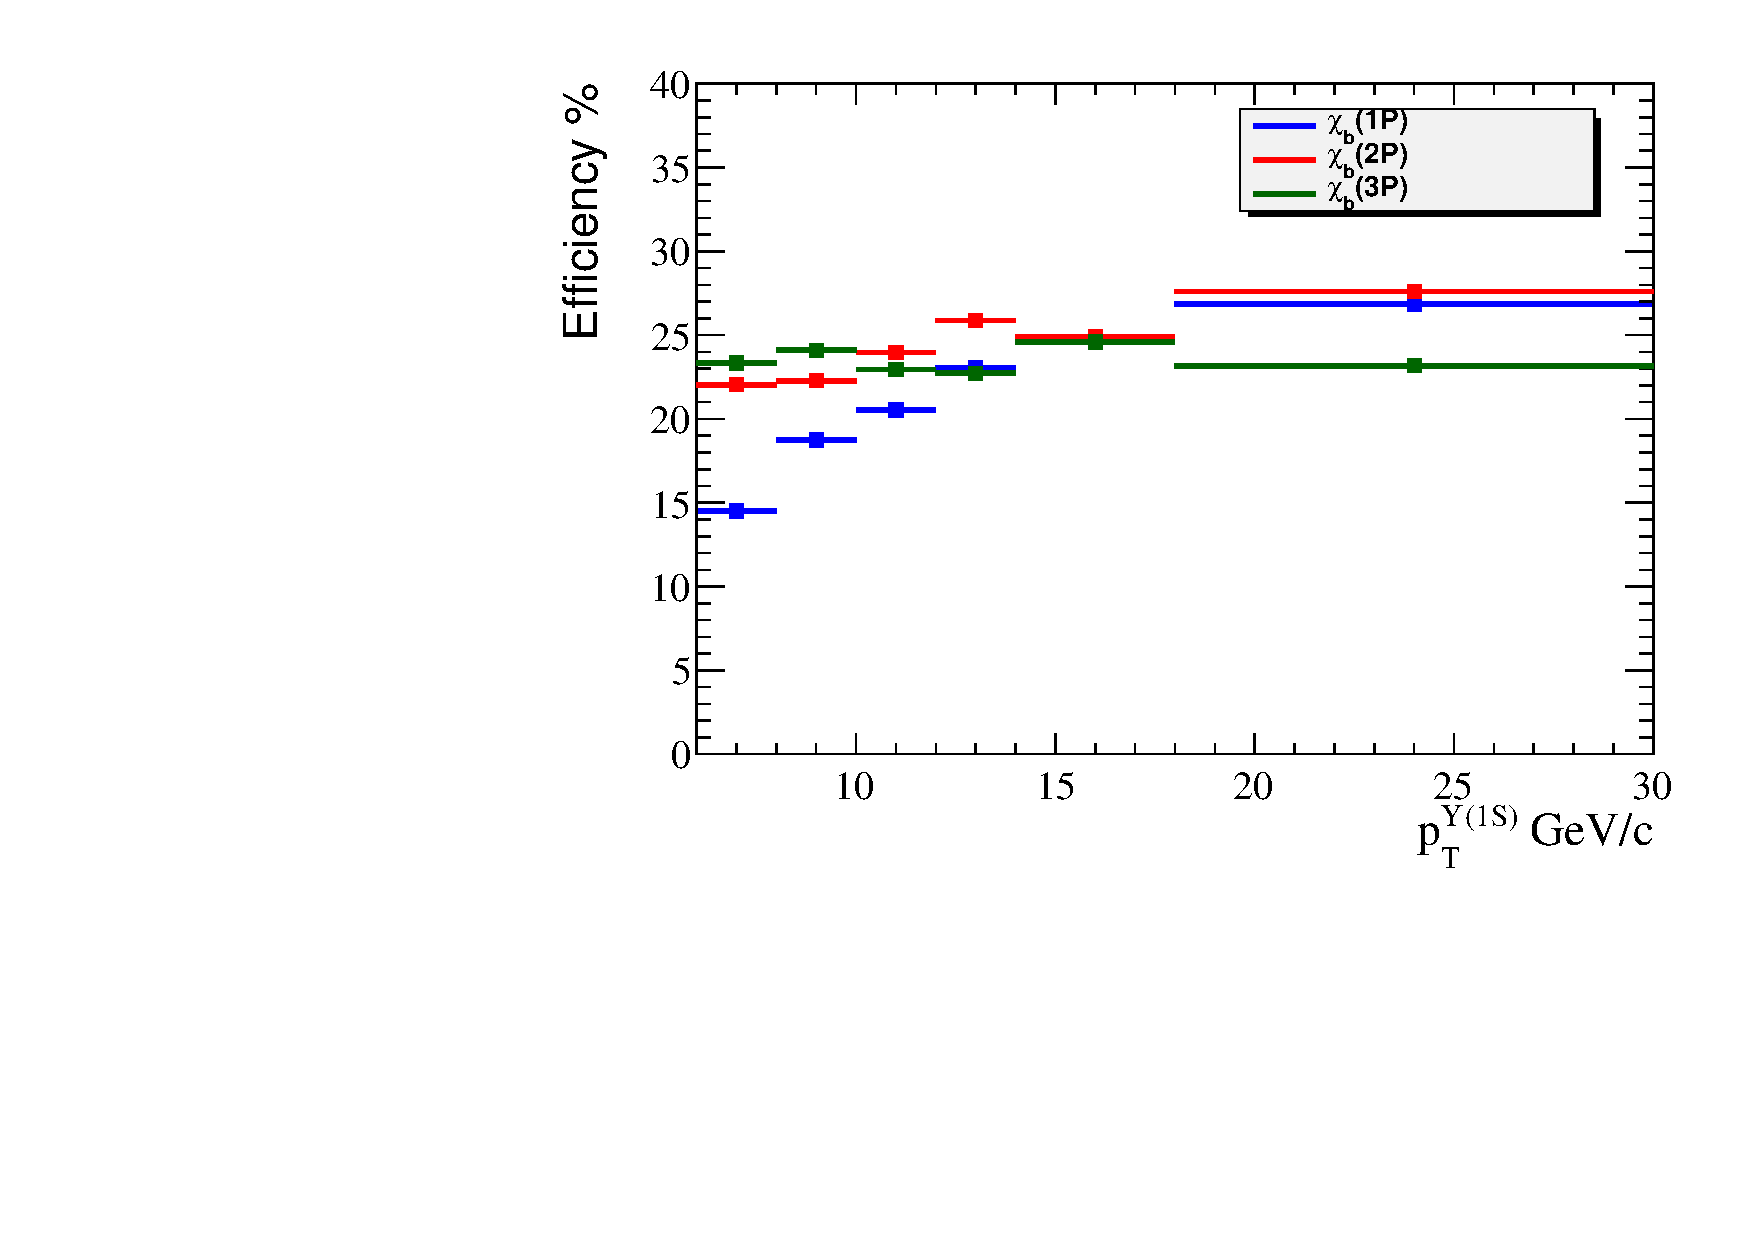
\includegraphics[width=0.5\linewidth]{mc_eff}
  \caption{
    \small  Monte-Carlo data. Fraction of \OneS originating from \chib decays for 
    different $p_{T}^{\OneS}$ intervals.
  }
  \label{fig:chib_fractions}
\end{figure}


\section{Determination of the \chib production cross section}
\label{sec:crosssec}

\begin{figure}[H]
  \centering
    \begin{subfigure}[b]{0.31\textwidth}
      \centering
      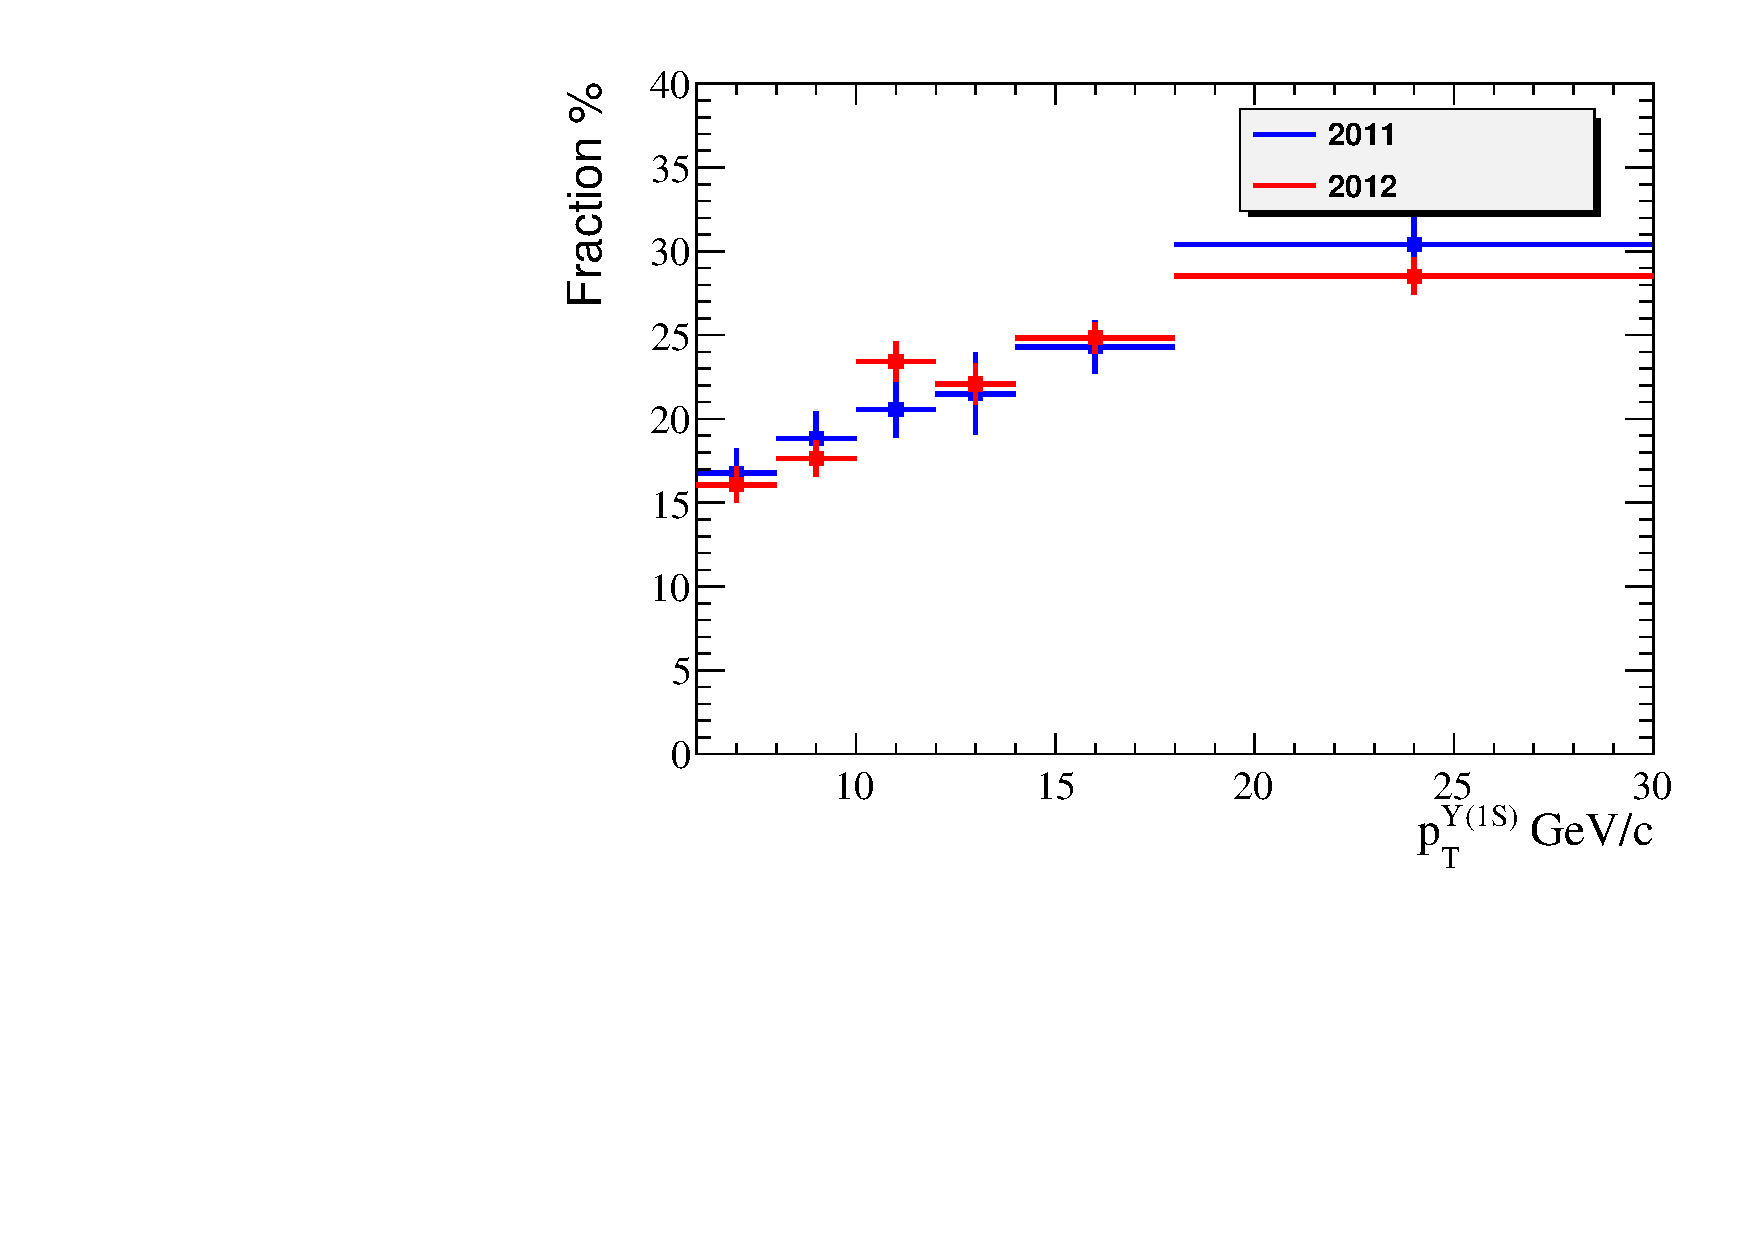
\includegraphics[width=\linewidth]{fractions/chib1p}
      \caption{from \chibOneP}
      \label{fig:fraction_1p}
    \end{subfigure}
    \begin{subfigure}[b]{0.31\textwidth}
      \centering
      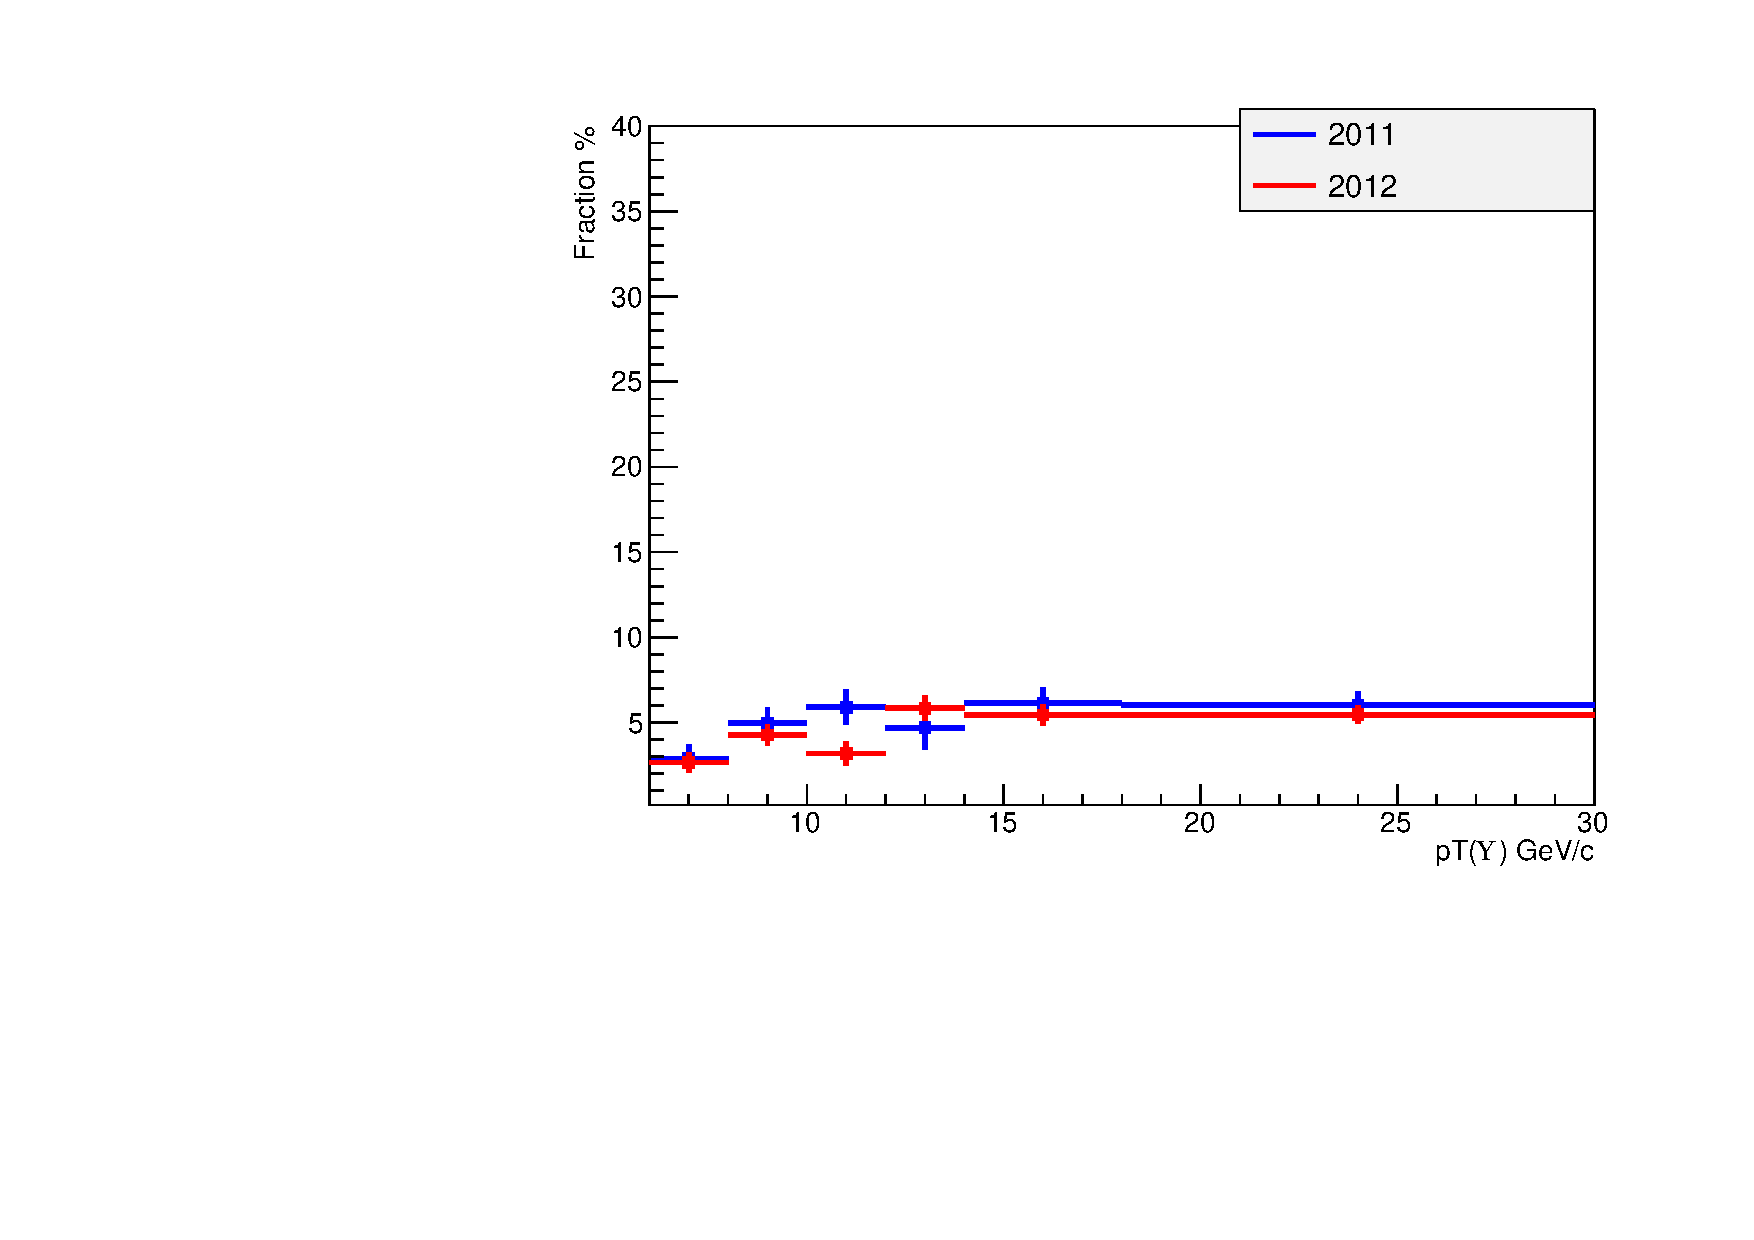
\includegraphics[width=\linewidth]{fractions/chib2p}
      \caption{from \chibTwoP}
      \label{fig:fraction_2p}
    \end{subfigure}
    \begin{subfigure}[b]{0.31\textwidth}
      \centering
      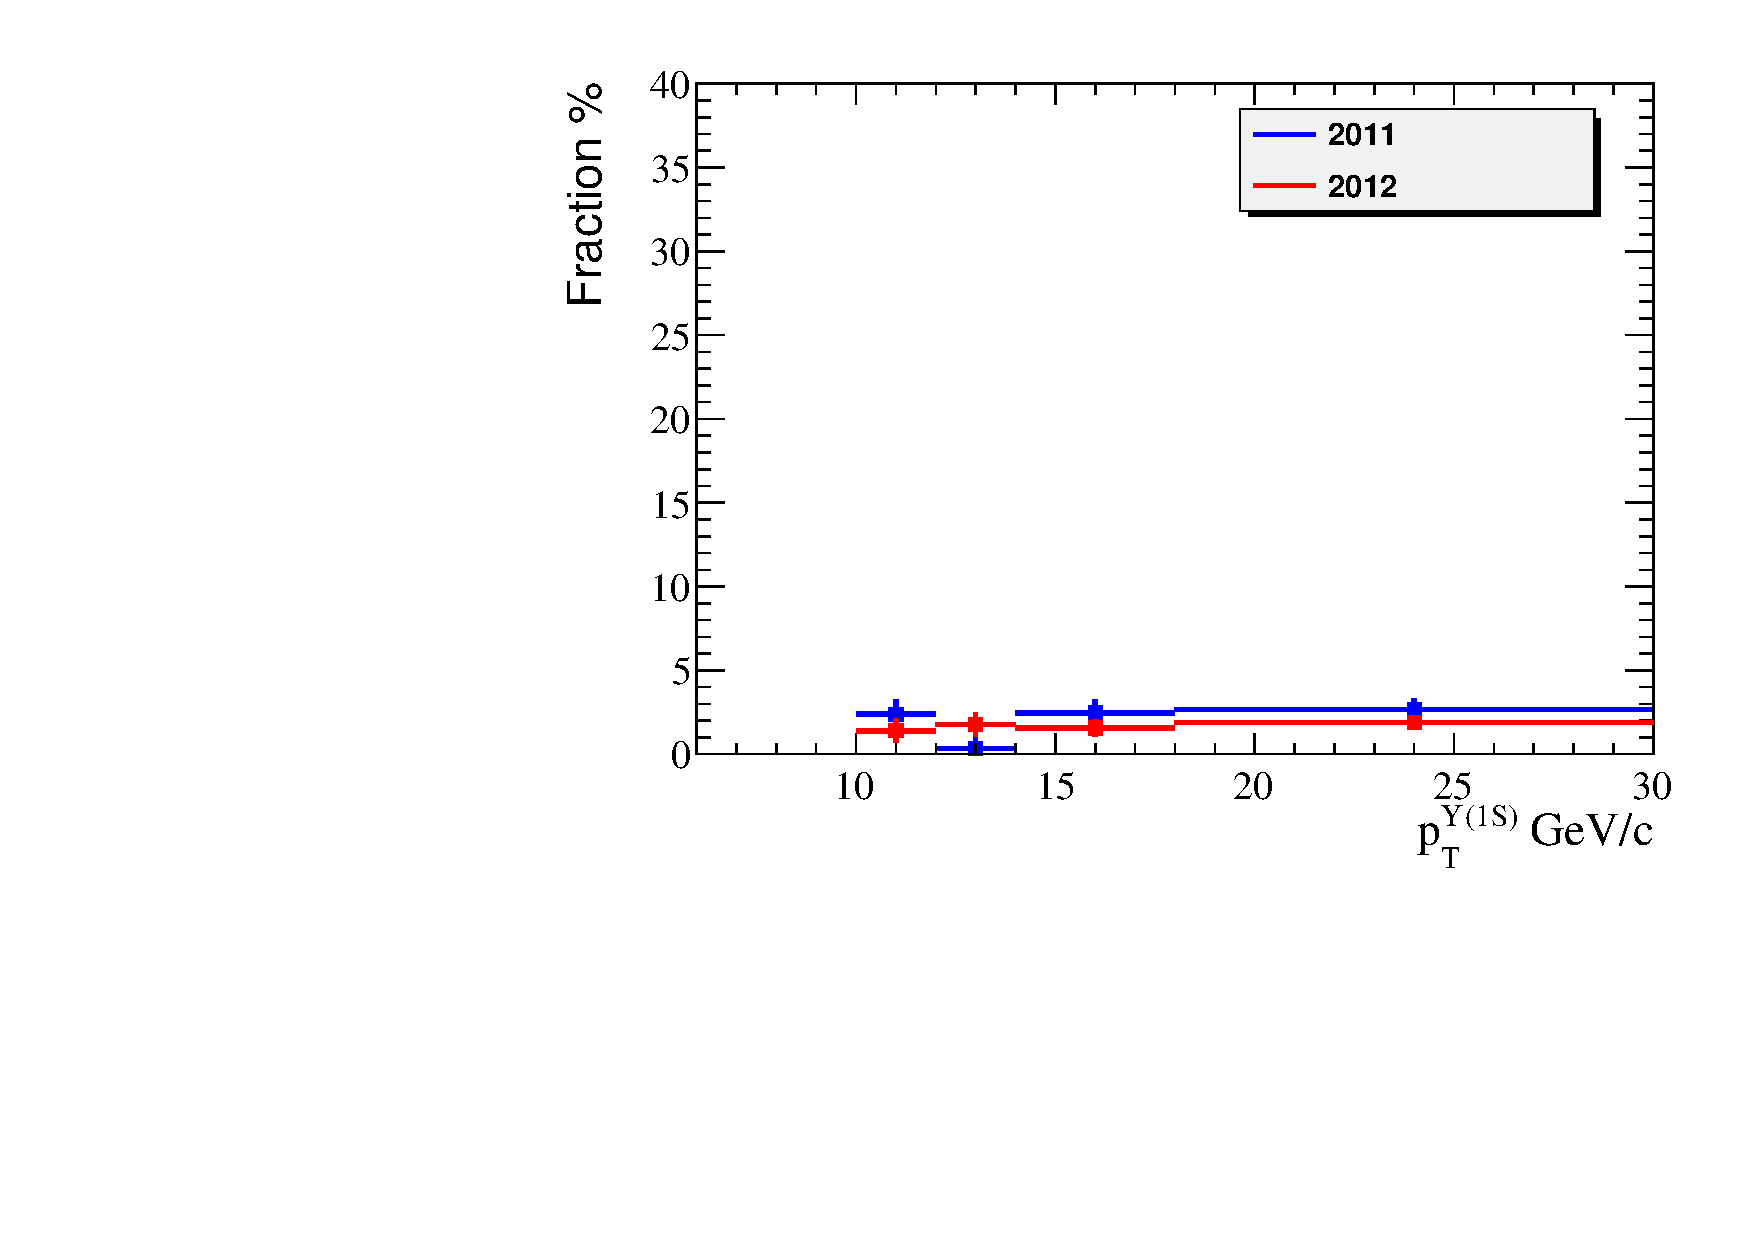
\includegraphics[width=\linewidth]{fractions/chib3p}
      \caption{from \chibThreeP}
      \label{fig:fraction_3p}
    \end{subfigure}    
  \caption{
    \small  Fraction of \OneS originating from \chib decays for 
    different $p_{T}^{\OneS}$ intervals.
  }
  \label{fig:chib_fractions}
\end{figure}



\section{Systematic Uncertainties}
\label{sec:syst}



\section{Determination of the $\chi_b$ masses}
\label{sec:masses}



\section{Conclusion}
\label{sec:conclusion}


% $Id: appendix.tex 37181 2013-06-11 18:22:48Z tgershon $
% ===============================================================================
% Purpose: appendix to the standard template: standard symbol alises from Ulrik
% Author: Tomasz Skwarnicki
% Created on: 2009-09-24
% ===============================================================================

\clearpage

{\noindent\bf\Large Appendices}

\appendix

\section{Fitting parameters summary}
\label{sec:FitingParameters}


\begin{table}[t]
\caption{\small Summary of fraction determination.}
\scalebox{0.5}{
\begin{tabular}{lccccccc}
\hline \hline
\multicolumn{7}{c}{\OneS transverse momentum interval in \gevc} \\
& 6 - 8 & 8 - 10 & 10 - 12 & 12 - 14 &  14 - 18 &   18 - 30 \\
\hline
\multicolumn{7}{c}{Parameters obtained by fitting data distributions $\sqs=7\tev$} \\
\hline
$N_{\chibOneP}^{rec}$  & 3160 $\pm$ 280 & 2620 $\pm$ 220 & 1750 $\pm$ 140 & 1140 $\pm$ 90 & 1250 $\pm$ 70 & 780 $\pm$ 40 \\
$N_{\chibTwoP}^{rec}$  & 750 $\pm$ 220 & 780 $\pm$ 150 & 550 $\pm$ 90 & 250 $\pm$ 60 & 270 $\pm$ 50 & 158 $\pm$ 20 \\
$N_{\chibThreeP}^{rec}$  &  &  & 230 $\pm$ 80 & 20 $\pm$ 60 & 120 $\pm$ 40 & 59 $\pm$ 14 \\
$\dm_{\chiboneOneP}$ in \mevcc  & 425.4 $\pm$ 2.2 & 424.2 $\pm$ 1.9 & 424.0 $\pm$ 1.9 & 430.3 $\pm$ 1.9 & 428.9 $\pm$ 1.5 & 429.3 $\pm$ 1.5 \\
$\dm_{\chiboneTwoP}$ in \mevcc  & 772 $\pm$ 12 & 784 $\pm$ 6 & 786 $\pm$ 6 & 784 $\pm$ 10 & 791 $\pm$ 6 & 796 $\pm$ 5 \\
$\dm_{\chiboneThreeP}$ in \mevcc  &  &  & 1047 $\pm$ 15 & 1030 $\pm$ 40 & 1035 $\pm$ 12 & 1065 $\pm$ 12 \\
\hline
$N_{\OneS}^{rec}$  & 128,900 $\pm$ 400  & 73,940 $\pm$ 320  & 41,390 $\pm$ 230  & 22,790 $\pm$ 170  & 19,660 $\pm$ 160  & 9610 $\pm$ 110  \\
\hline \hline
\multicolumn{7}{c}{Parameters obtained by fitting data distributions $\sqs=8\tev$} \\
\hline
$N_{\chibOneP}^{rec}$  & 6500 $\pm$ 400 & 5510 $\pm$ 320 & 4410 $\pm$ 230 & 2630 $\pm$ 140 & 2810 $\pm$ 100 & 1800 $\pm$ 70 \\
$N_{\chibTwoP}^{rec}$  & 1490 $\pm$ 340 & 1650 $\pm$ 210 & 650 $\pm$ 140 & 700 $\pm$ 90 & 600 $\pm$ 70 & 348 $\pm$ 35 \\
$N_{\chibThreeP}^{rec}$  &  &  & 290 $\pm$ 150 & 210 $\pm$ 80 & 170 $\pm$ 60 & 103 $\pm$ 22 \\
$\dm_{\chiboneOneP}$ in \mevcc  & 426.0 $\pm$ 1.5 & 424.4 $\pm$ 1.3 & 425.9 $\pm$ 1.1 & 424.3 $\pm$ 1.2 & 427.6 $\pm$ 1.0 & 430.6 $\pm$ 1.0 \\
$\dm_{\chiboneTwoP}$ in \mevcc  & 774 $\pm$ 9 & 781 $\pm$ 6 & 794 $\pm$ 9 & 801 $\pm$ 5 & 789 $\pm$ 4 & 801 $\pm$ 4 \\
$\dm_{\chiboneThreeP}$ in \mevcc  &  &  & 1049 $\pm$ 22 & 1036 $\pm$ 18 & 1067 $\pm$ 17 & 1084 $\pm$ 6 \\
\hline
$N_{\OneS}^{rec}$  & 277,000 $\pm$ 600  & 162,500 $\pm$ 500  & 91,610 $\pm$ 350  & 51,270 $\pm$ 260  & 45,350 $\pm$ 240  & 23,540 $\pm$ 180 \\

\hline \hline
\multicolumn{7}{c}{Parameters obtained by counting MC matched events for \chiboneOneP decay} \\
\hline
$N_{ \chiboneOneP }^{MC}$  & 6172 & 5345 & 3653 & 2266 & 2131 & 1113 \\
$N_{\OneS}^{MC}$  & 42,587 & 28,398 & 17,078 & 9632 & 8237 & 3922 \\
$\eps_{ \chiboneOneP }^{MC}$ \%  & 14.5 & 18.8 & 21.4 & 23.5 & 25.9 & 28.4 \\\hline \hline
\multicolumn{7}{c}{Parameters obtained by counting MC matched events for \chibtwoOneP decay} \\
\hline
$N_{ \chibtwoOneP }^{MC}$  & 4327 & 2676 & 1298 & 645 & 467 & 164 \\
$N_{\OneS}^{MC}$  & 29,792 & 14,325 & 6594 & 2850 & 1952 & 648 \\
$\eps_{ \chibtwoOneP }^{MC}$ \%  & 14.5 & 18.7 & 19.7 & 22.6 & 23.9 & 25.3 \\\hline \hline
\multicolumn{7}{c}{Parameters obtained by counting MC matched events for \chiboneTwoP decay} \\
\hline
$N_{ \chiboneTwoP }^{MC}$  & 4648 & 3273 & 2041 & 1155 & 1016 & 524 \\
$N_{\OneS}^{MC}$  & 20,091 & 13,810 & 8176 & 4426 & 3974 & 1898 \\
$\eps_{ \chiboneTwoP }^{MC}$ \%  & 23.1 & 23.7 & 25.0 & 26.1 & 25.6 & 27.6 \\\hline \hline
\multicolumn{7}{c}{Parameters obtained by counting MC matched events for \chibtwoTwoP decay} \\
\hline
$N_{ \chibtwoTwoP }^{MC}$  & 3712 & 1712 & 848 & 431 & 269 & 106 \\
$N_{\OneS}^{MC}$  & 17,731 & 8212 & 3694 & 1679 & 1110 & 384 \\
$\eps_{ \chibtwoTwoP }^{MC}$ \%  & 20.9 & 20.8 & 23.0 & 25.7 & 24.2 & 27.6 \\\hline \hline
\multicolumn{7}{c}{Parameters obtained by counting MC matched events for \chiboneThreeP decay} \\
\hline
$N_{ \chiboneThreeP }^{MC}$  & 4629 & 3120 & 1772 & 1066 & 884 & 415 \\
$N_{\OneS}^{MC}$  & 18,486 & 12,359 & 7298 & 4174 & 3581 & 1646 \\
$\eps_{ \chiboneThreeP }^{MC}$ \%  & 25.0 & 25.2 & 24.3 & 25.5 & 24.7 & 25.2 \\\hline \hline
\multicolumn{7}{c}{Parameters obtained by counting MC matched events for \chibtwoThreeP decay} \\
\hline
$N_{ \chibtwoThreeP }^{MC}$  & 2598 & 1282 & 524 & 223 & 192 & 49 \\
$N_{\OneS}^{MC}$  & 12,003 & 5587 & 2425 & 1119 & 784 & 232 \\
$\eps_{ \chibtwoThreeP }^{MC}$ \%  & 21.6 & 22.9 & 21.6 & 19.9 & 24.5 & 21.1 \\
\hline \hline
\multicolumn{7}{c}{Average MC efficiency of \chibone and \chibtwo \mevcc in \%} \\
\hline
$\eps_{\chibOneP}^{MC}$  & 14.5 & 18.8 & 20.5 & 23.1 & 24.9 & 26.8 \\
$\eps_{\chibTwoP}^{MC}$  & 22.0 & 22.3 & 24.0 & 25.9 & 24.9 & 27.6 \\
$\eps_{\chibThreeP}^{MC}$  & 23.3 & 24.1 & 22.9 & 22.7 & 24.6 & 23.2 \\
\hline \hline
\multicolumn{7}{c}{Parameters obtained by fitting MC distributions in \mevcc} \\
\hline
$\dm_{\chiboneOneP}$  & 428.18 $\pm$ 0.34 & 427.5 $\pm$ 0.4 & 427.3 $\pm$ 0.4 & 427.2 $\pm$ 0.5 & 427.4 $\pm$ 0.5 & 428.0 $\pm$ 0.6 \\
$\dm_{\chibtwoOneP}$  & 448.2 $\pm$ 0.5 & 447.2 $\pm$ 0.6 & 447.3 $\pm$ 0.7 & 447.0 $\pm$ 0.9 & 446.1 $\pm$ 1.1 & 446.1 $\pm$ 1.4 \\
$\dm_{\chiboneTwoP}$  & 786.4 $\pm$ 0.6 & 786.5 $\pm$ 0.7 & 786.7 $\pm$ 0.9 & 786.5 $\pm$ 1.0 & 789.0 $\pm$ 1.0 & 790.2 $\pm$ 1.3 \\
$\dm_{\chibtwoTwoP}$  & 800.8 $\pm$ 0.7 & 800.9 $\pm$ 1.0 & 799.5 $\pm$ 1.2 & 802.5 $\pm$ 1.7 & 799.9 $\pm$ 1.9 & 802.8 $\pm$ 3.2 \\
$\dm_{\chiboneThreeP}$  & 1046.2 $\pm$ 0.7 & 1046.8 $\pm$ 0.8 & 1047.9 $\pm$ 1.0 & 1047.4 $\pm$ 1.3 & 1049.5 $\pm$ 1.3 & 1050.9 $\pm$ 1.9 \\
$\dm_{\chibtwoThreeP}$  & 1058.0 $\pm$ 1.0 & 1055.9 $\pm$ 1.2 & 1058.1 $\pm$ 2.1 & 1059.6 $\pm$ 2.8 & 1063.9 $\pm$ 2.8 & 1061 $\pm$ 7 \\
\hline
$\sigma_{\chiboneOneP}$  & 23.14 $\pm$ 0.35 & 22.3 $\pm$ 0.4 & 21.1 $\pm$ 0.4 & 19.9 $\pm$ 0.5 & 19.4 $\pm$ 0.5 & 19.0 $\pm$ 0.6 \\
$\sigma_{\chibtwoOneP}$  & 24.2 $\pm$ 0.5 & 23.3 $\pm$ 0.6 & 21.4 $\pm$ 0.7 & 20.7 $\pm$ 1.0 & 22.4 $\pm$ 0.9 & 15.8 $\pm$ 1.3 \\
$\sigma_{\chiboneTwoP}$  & 34.2 $\pm$ 0.8 & 33.5 $\pm$ 0.8 & 32.9 $\pm$ 1.0 & 32.3 $\pm$ 0.8 & 30.7 $\pm$ 0.8 & 29.2 $\pm$ 1.2 \\
$\sigma_{\chibtwoTwoP}$  & 37.5 $\pm$ 0.7 & 33.5 $\pm$ 1.1 & 32.6 $\pm$ 1.0 & 33.1 $\pm$ 1.5 & 31.6 $\pm$ 1.5 & 32.1 $\pm$ 2.6 \\
$\sigma_{\chiboneThreeP}$  & 47.2 $\pm$ 0.6 & 45.9 $\pm$ 0.7 & 43.4 $\pm$ 0.9 & 43.3 $\pm$ 1.1 & 42.3 $\pm$ 1.0 & 40.2 $\pm$ 1.5 \\
$\sigma_{\chibtwoThreeP}$  & 49.0 $\pm$ 0.9 & 42.0 $\pm$ 1.2 & 43.1 $\pm$ 2.1 & 40.2 $\pm$ 3.0 & 38.1 $\pm$ 2.4 & 41 $\pm$ 6 \\
\hline \hline
\multicolumn{7}{c}{Fraction of \OneS in \% for \sqs=7\tev} \\
\hline
from $\chibOneP$  & 16.9 $\pm$ 1.5 & 18.9 $\pm$ 1.6 & 20.6 $\pm$ 1.7 & 21.7 $\pm$ 1.7 & 25.6 $\pm$ 1.4 & 30.4 $\pm$ 1.7 \\
from $\chibTwoP$  & 2.7 $\pm$ 0.8 & 4.7 $\pm$ 0.9 & 5.5 $\pm$ 0.9 & 4.3 $\pm$ 1.0 & 5.6 $\pm$ 1.0 & 5.9 $\pm$ 0.8 \\
from $\chibThreeP$  &  &  & 2.4 $\pm$ 0.9 & 0.3 $\pm$ 1.1 & 2.5 $\pm$ 0.8 & 2.7 $\pm$ 0.7 \\
\hline \hline
\multicolumn{7}{c}{Fraction of \OneS in \% for \sqs=8\tev} \\
\hline
from $\chibOneP$  & 16.2 $\pm$ 1.1 & 18.1 $\pm$ 1.1 & 23.4 $\pm$ 1.2 & 22.2 $\pm$ 1.2 & 24.9 $\pm$ 0.9 & 28.5 $\pm$ 1.1 \\
from $\chibTwoP$  & 2.4 $\pm$ 0.6 & 4.6 $\pm$ 0.6 & 3.0 $\pm$ 0.6 & 5.3 $\pm$ 0.7 & 5.3 $\pm$ 0.6 & 5.4 $\pm$ 0.5 \\
from $\chibThreeP$  &  &  & 1.4 $\pm$ 0.7 & 1.8 $\pm$ 0.7 & 1.6 $\pm$ 0.5 & 1.9 $\pm$ 0.4 \\
\hline \hline
\end{tabular}
}
\label{tab:fit_summary}
\end{table}


\begin{figure}[ht]
  \centering
    \begin{subfigure}[b]{\textwidth}
      \centering
      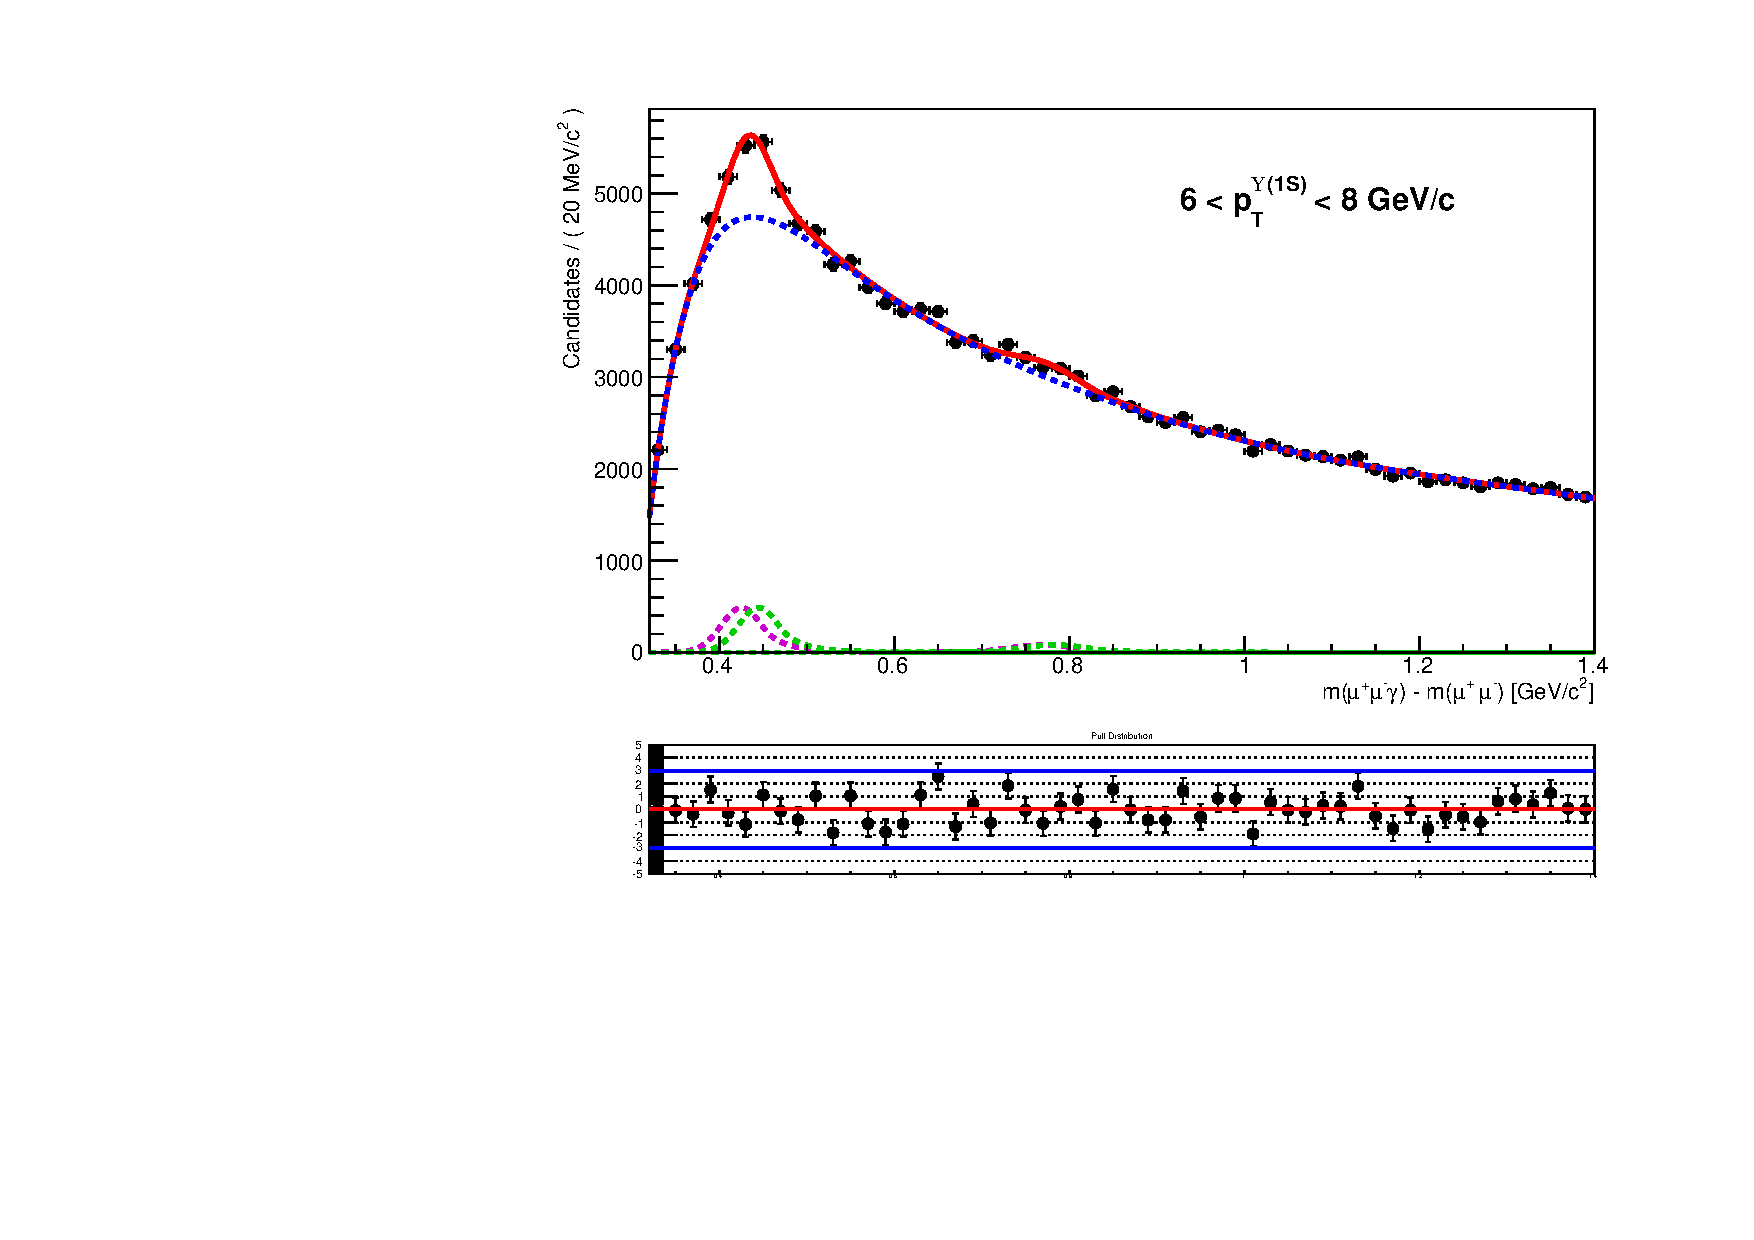
\includegraphics[width=0.31\linewidth]{chib_fits/fit_chib_2011_6_8}
      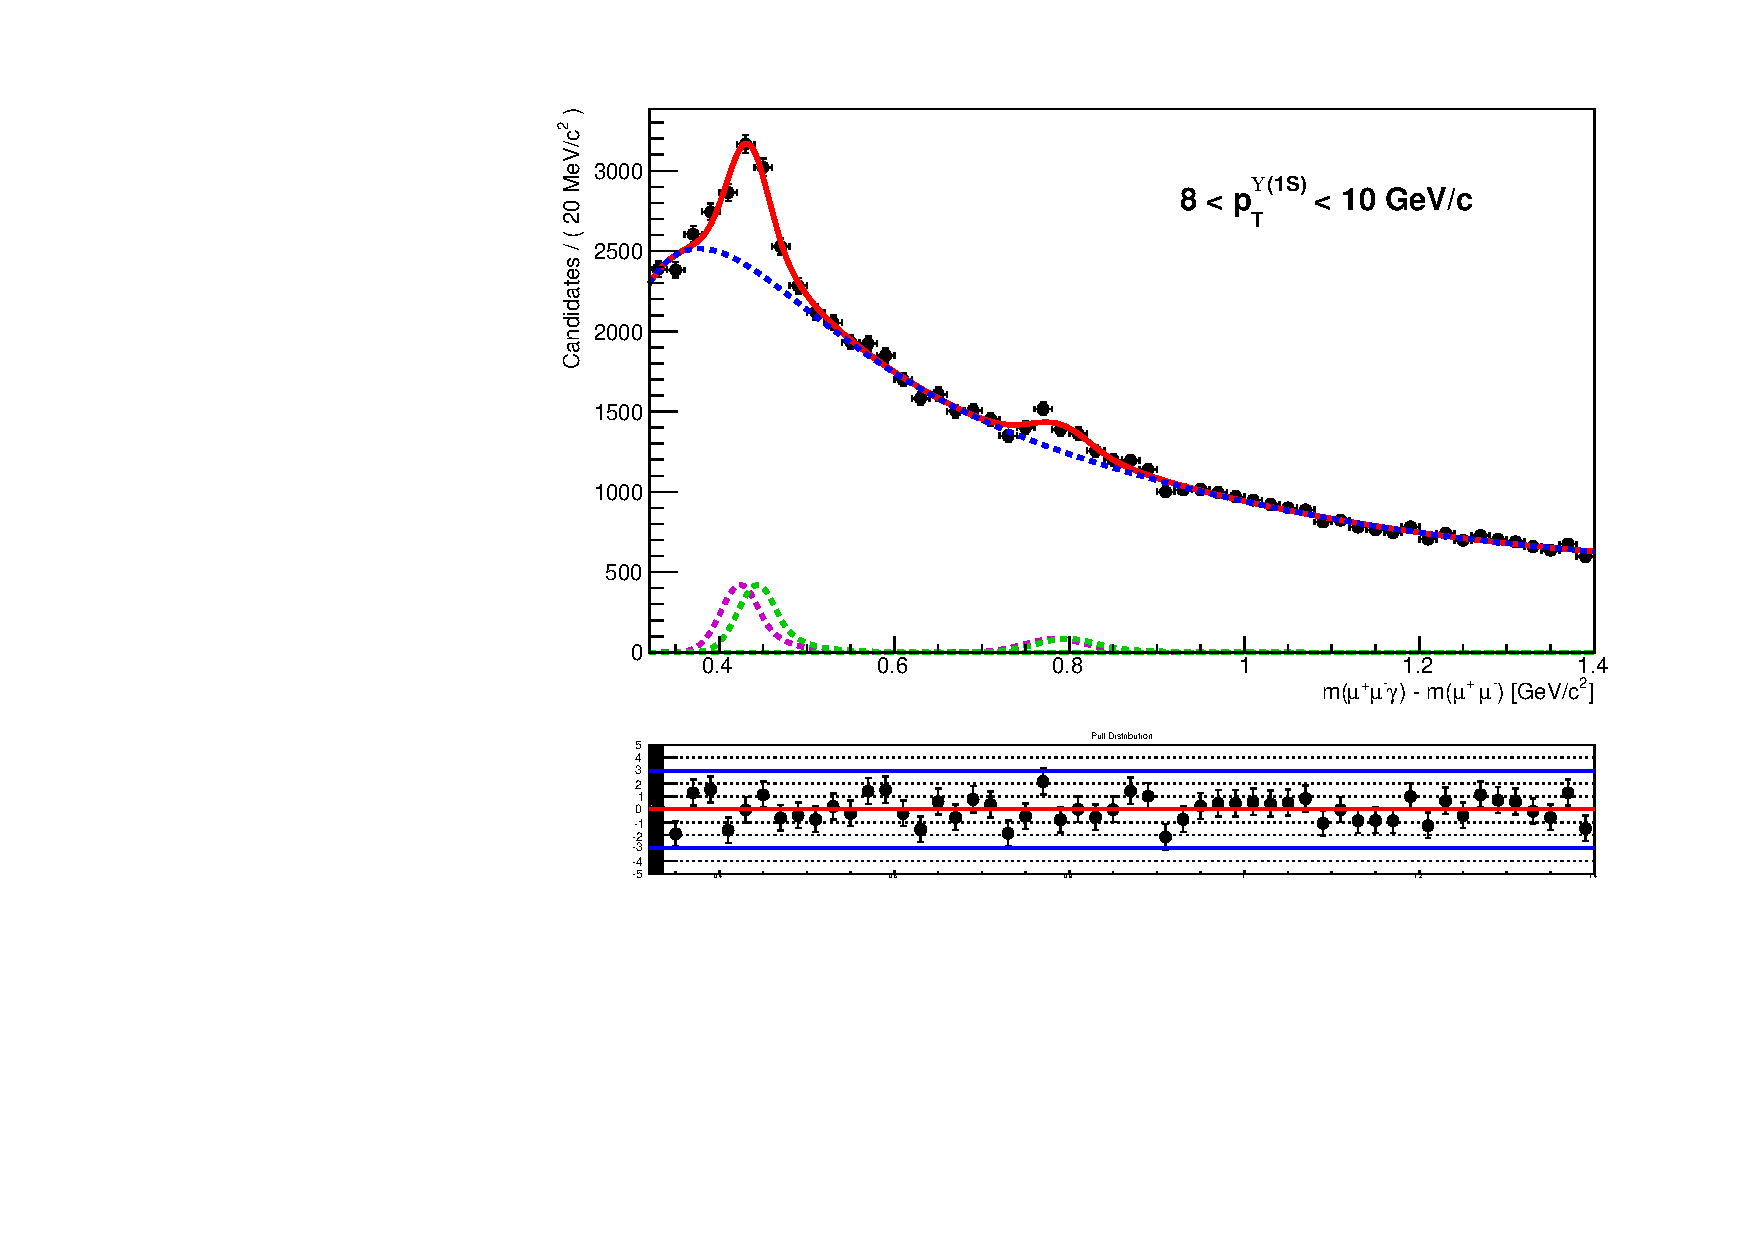
\includegraphics[width=0.31\linewidth]{chib_fits/fit_chib_2011_8_10}
      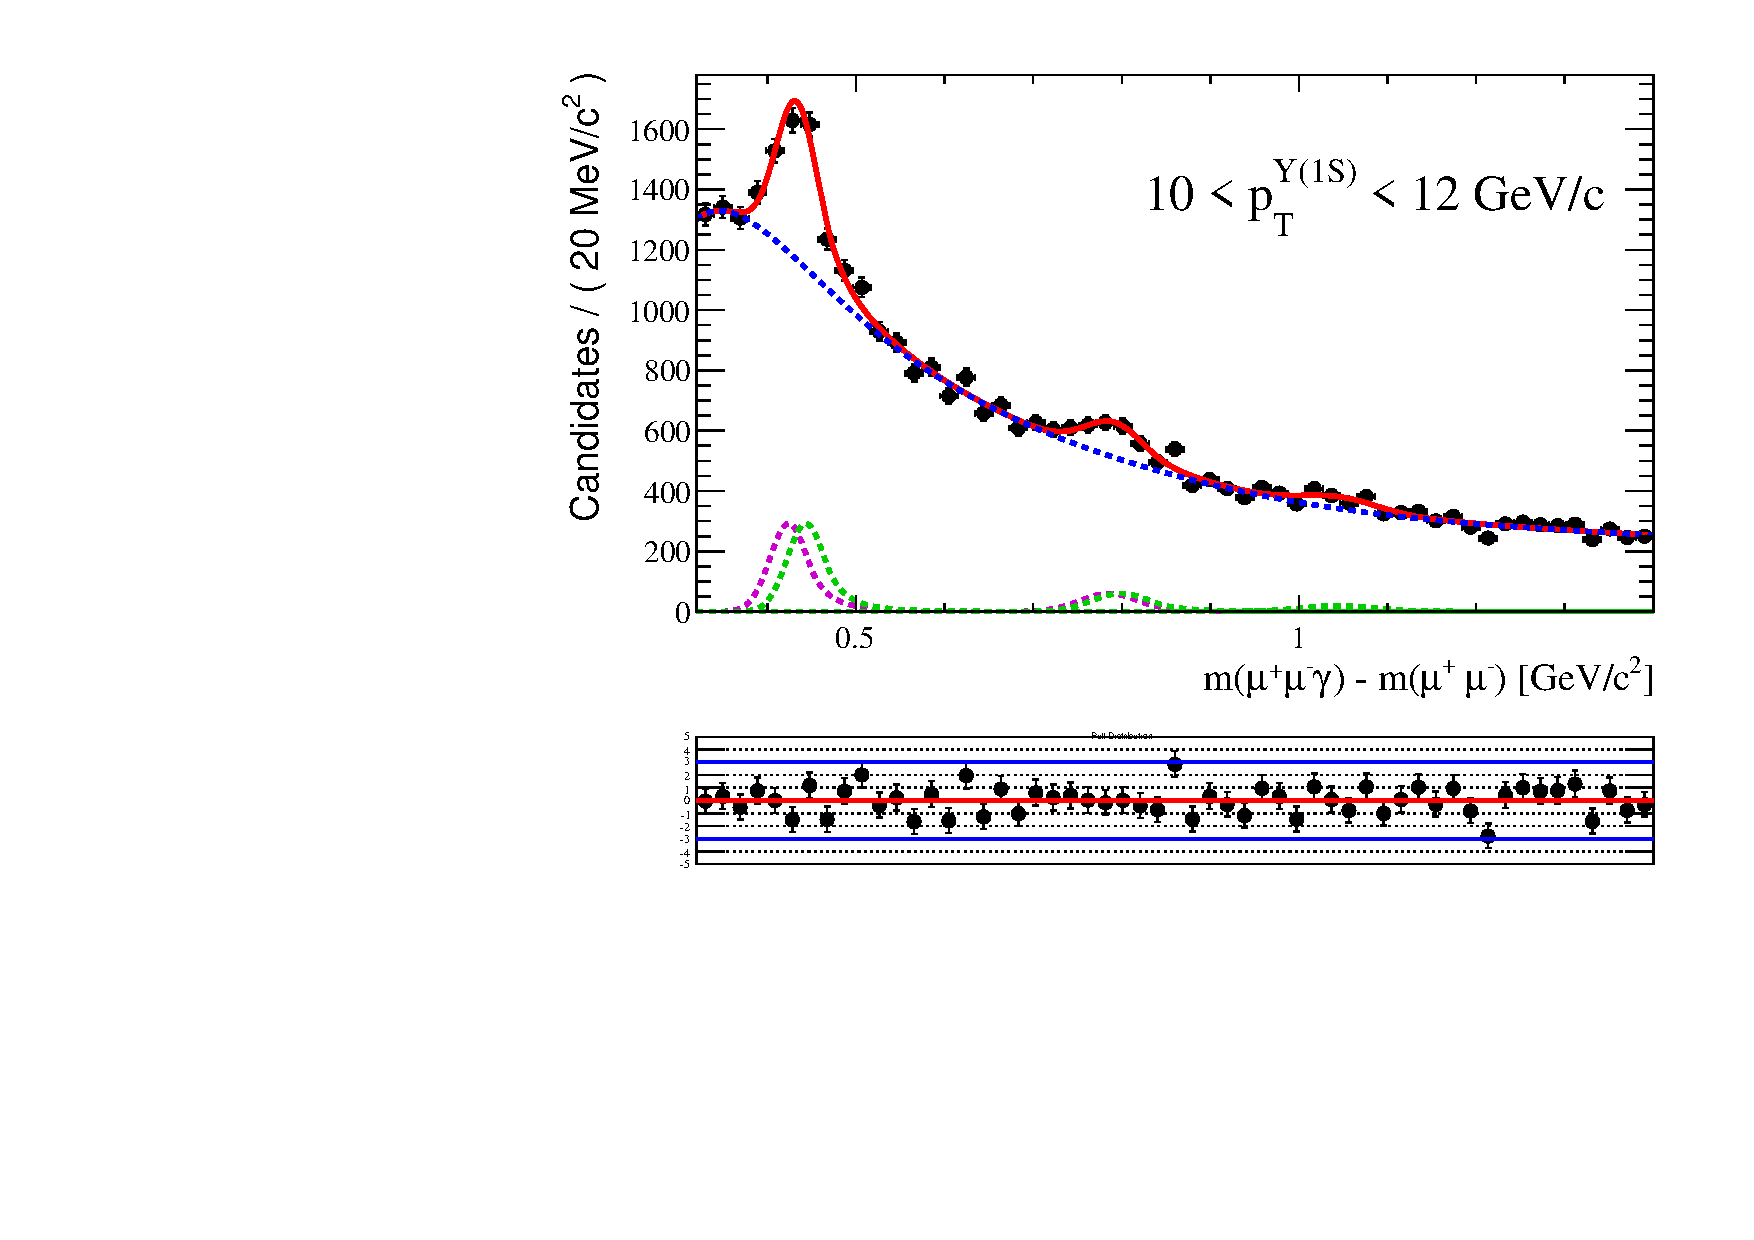
\includegraphics[width=0.31\linewidth]{chib_fits/fit_chib_2011_10_12}
      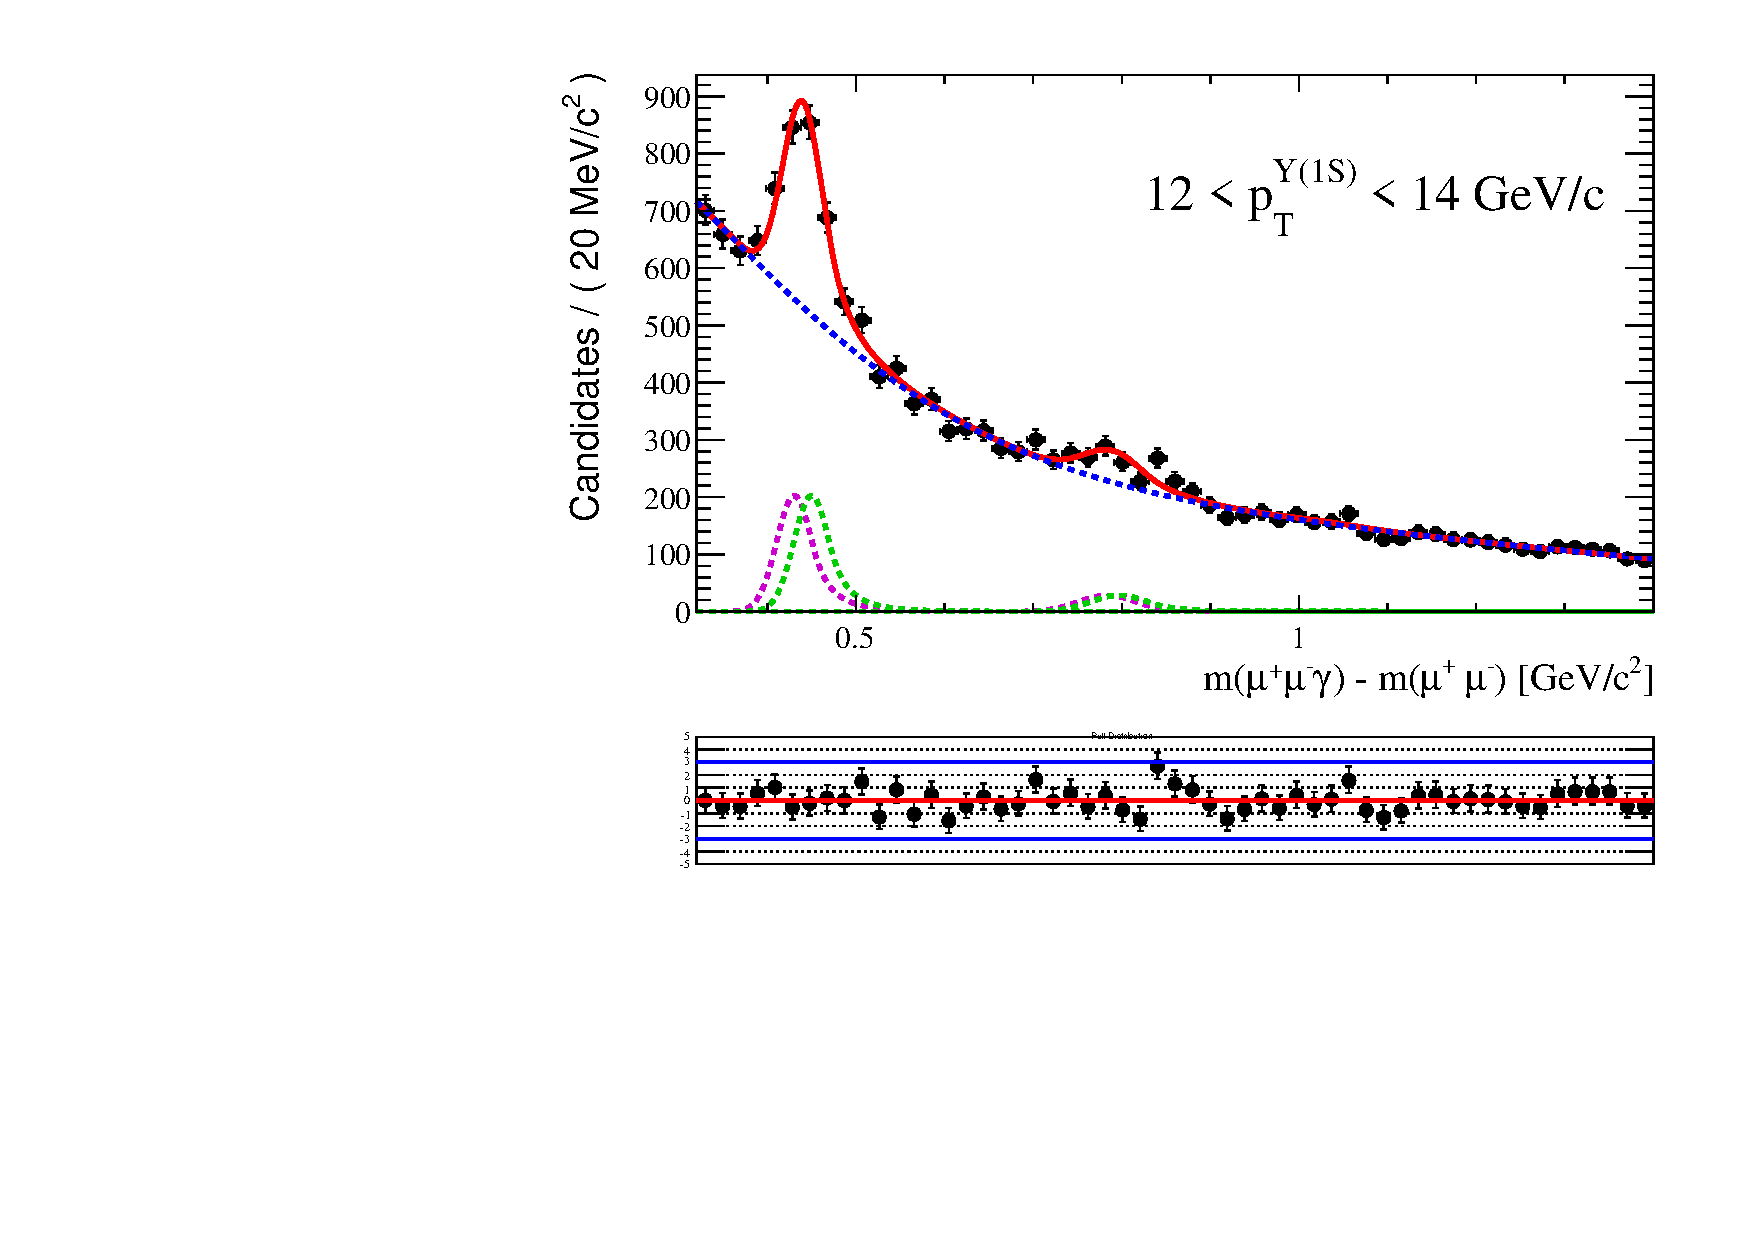
\includegraphics[width=0.31\linewidth]{chib_fits/fit_chib_2011_12_14}
      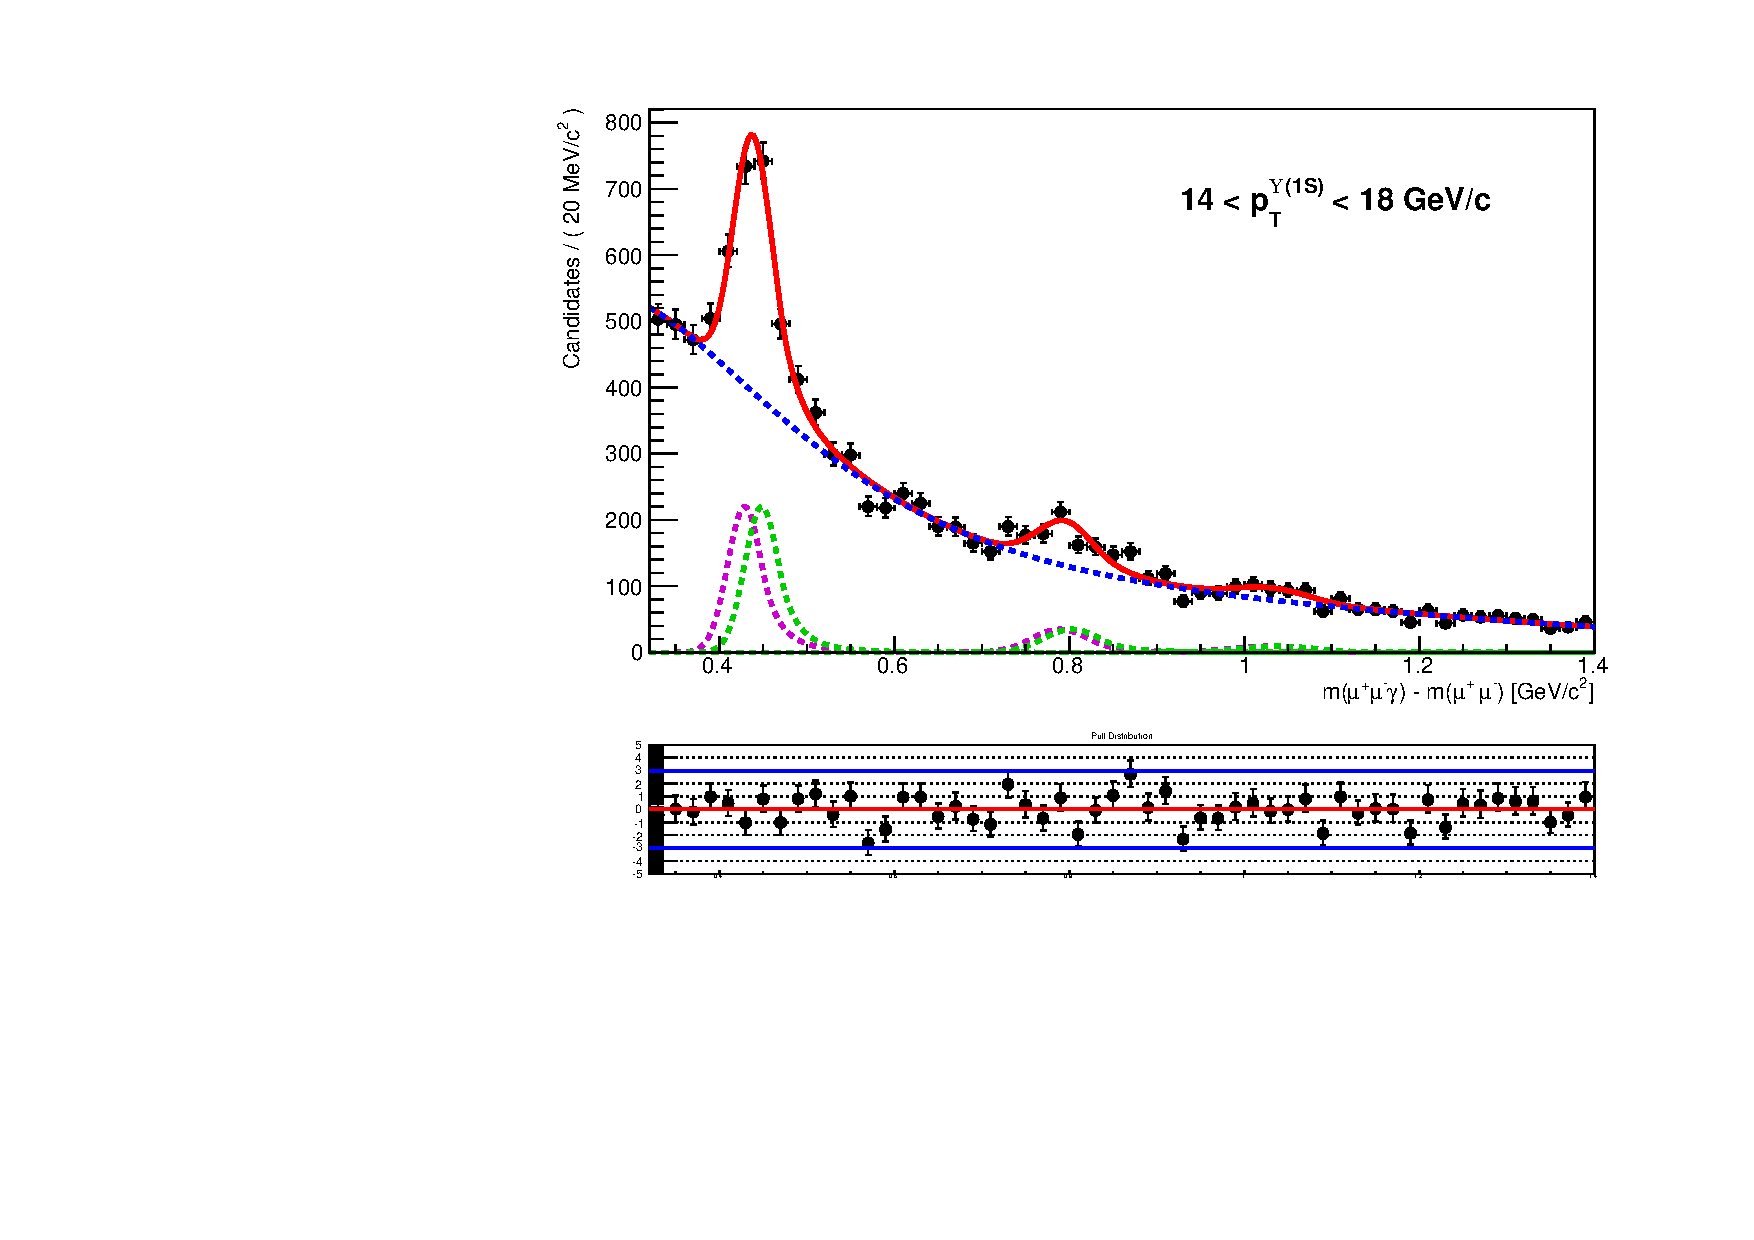
\includegraphics[width=0.31\linewidth]{chib_fits/fit_chib_2011_14_18}
      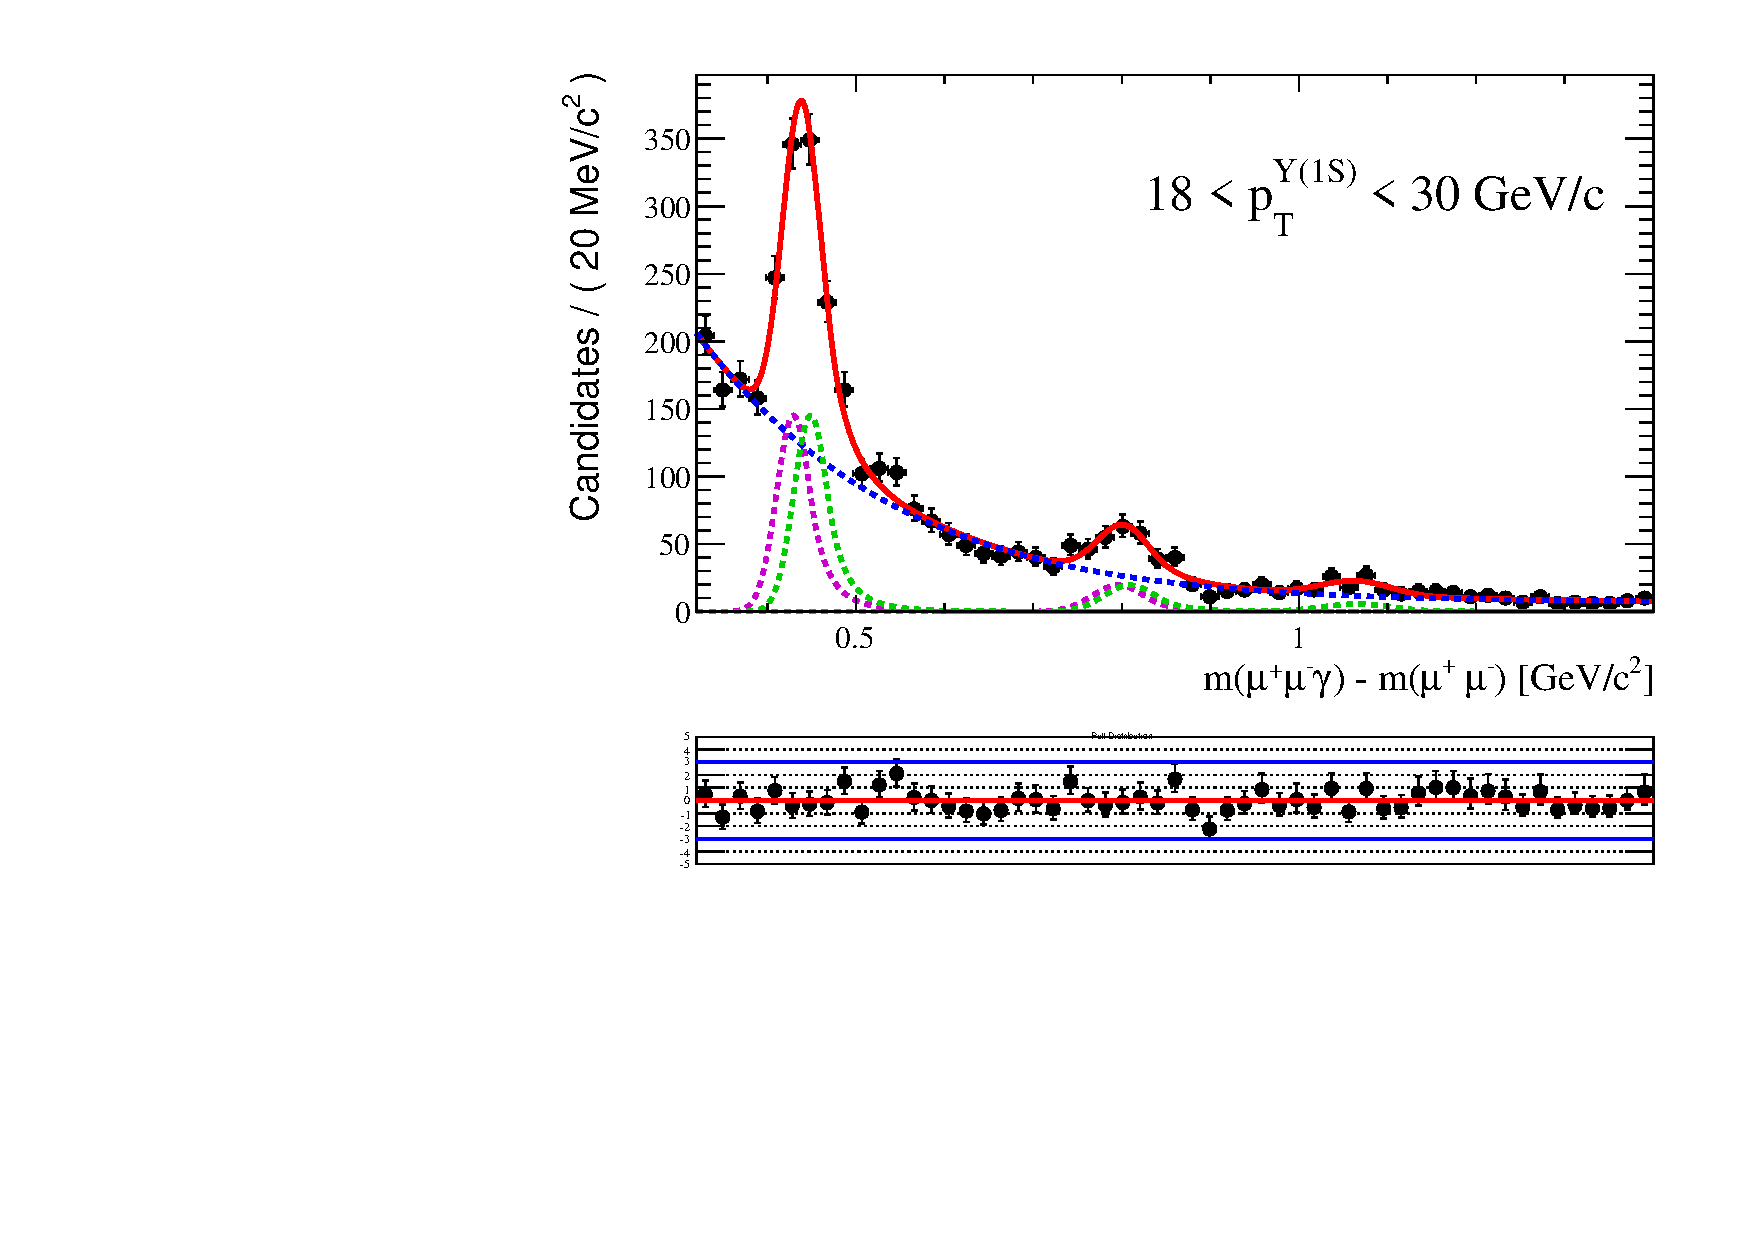
\includegraphics[width=0.31\linewidth]{chib_fits/fit_chib_2011_18_30}
      \caption{\sqs=7\tev (2011)}
      \label{fig:chib_fits_2011}
    \end{subfigure}
    \begin{subfigure}[b]{\textwidth}
      \centering
      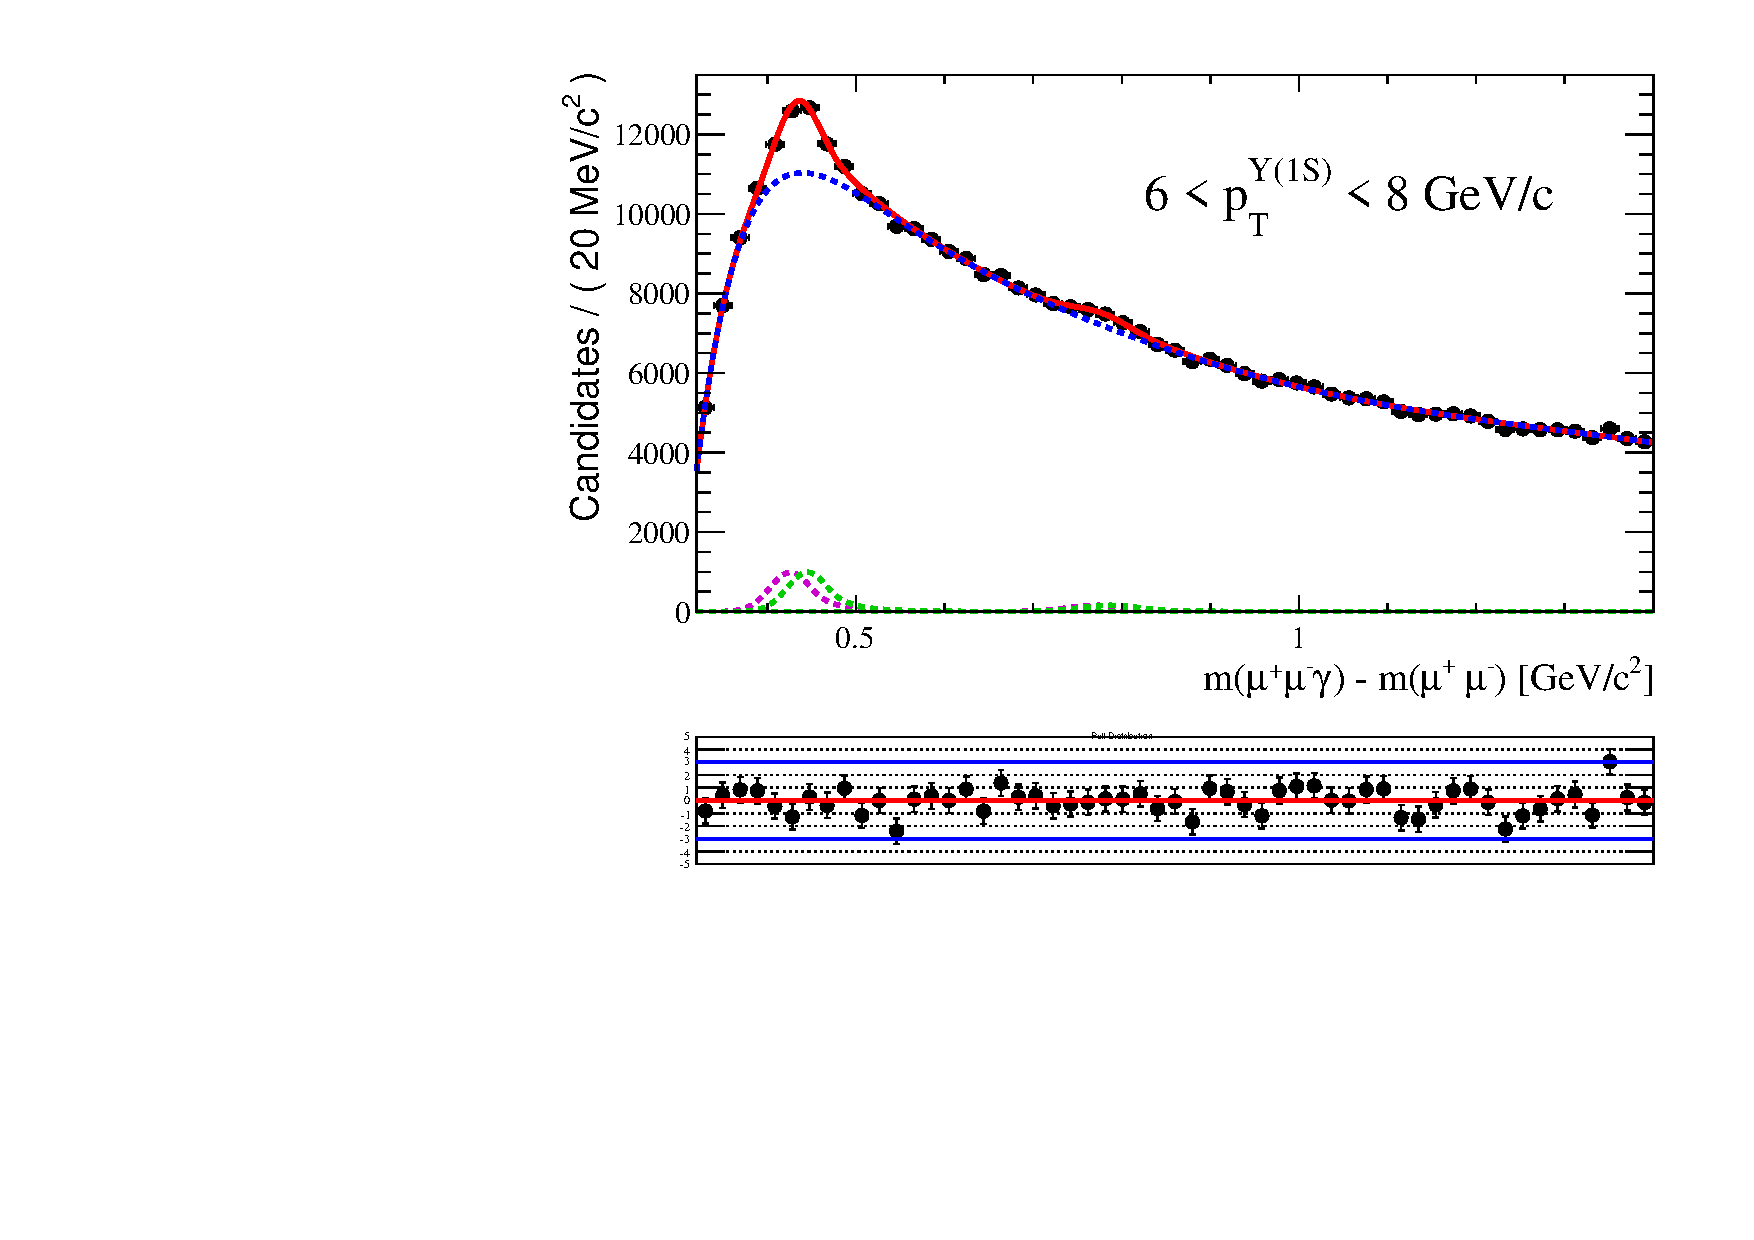
\includegraphics[width=0.31\linewidth]{chib_fits/fit_chib_2012_6_8}
      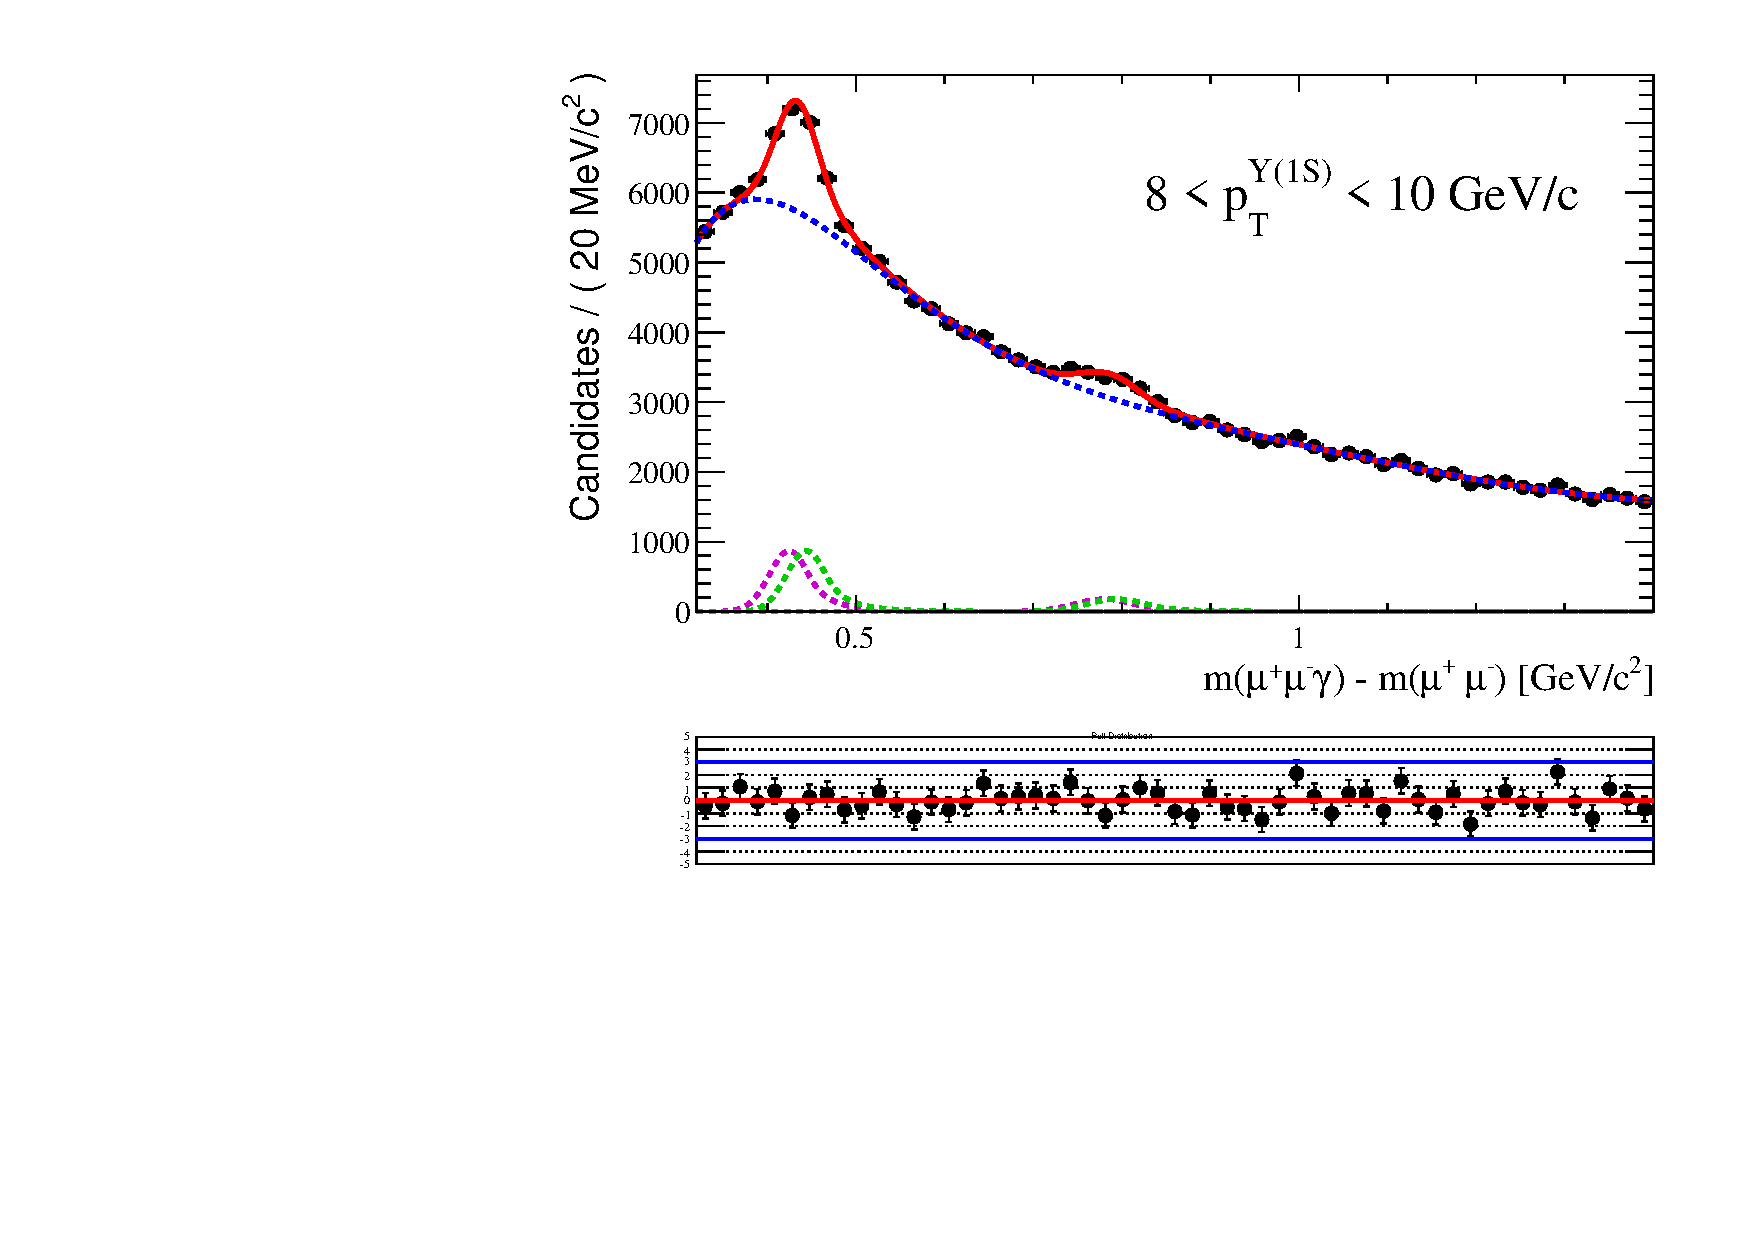
\includegraphics[width=0.31\linewidth]{chib_fits/fit_chib_2012_8_10}
      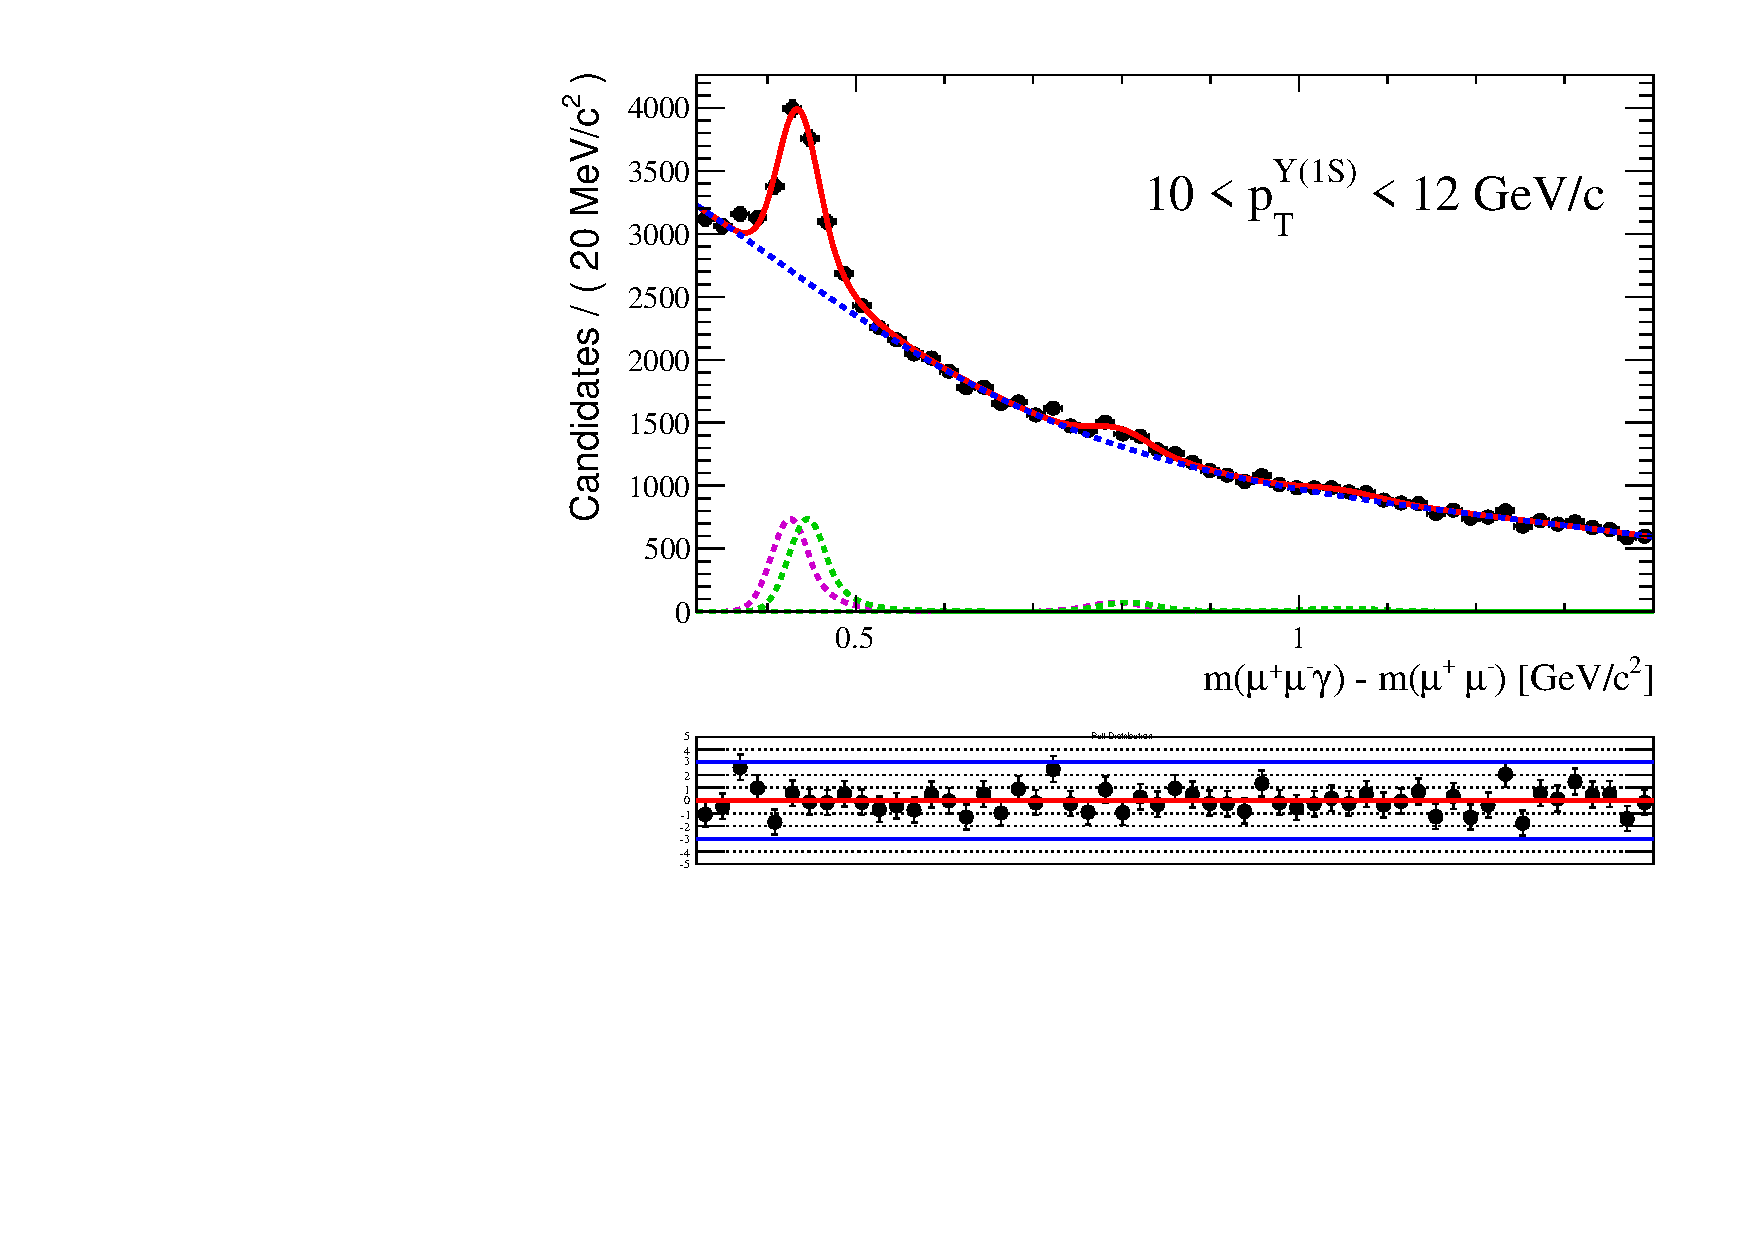
\includegraphics[width=0.31\linewidth]{chib_fits/fit_chib_2012_10_12}
      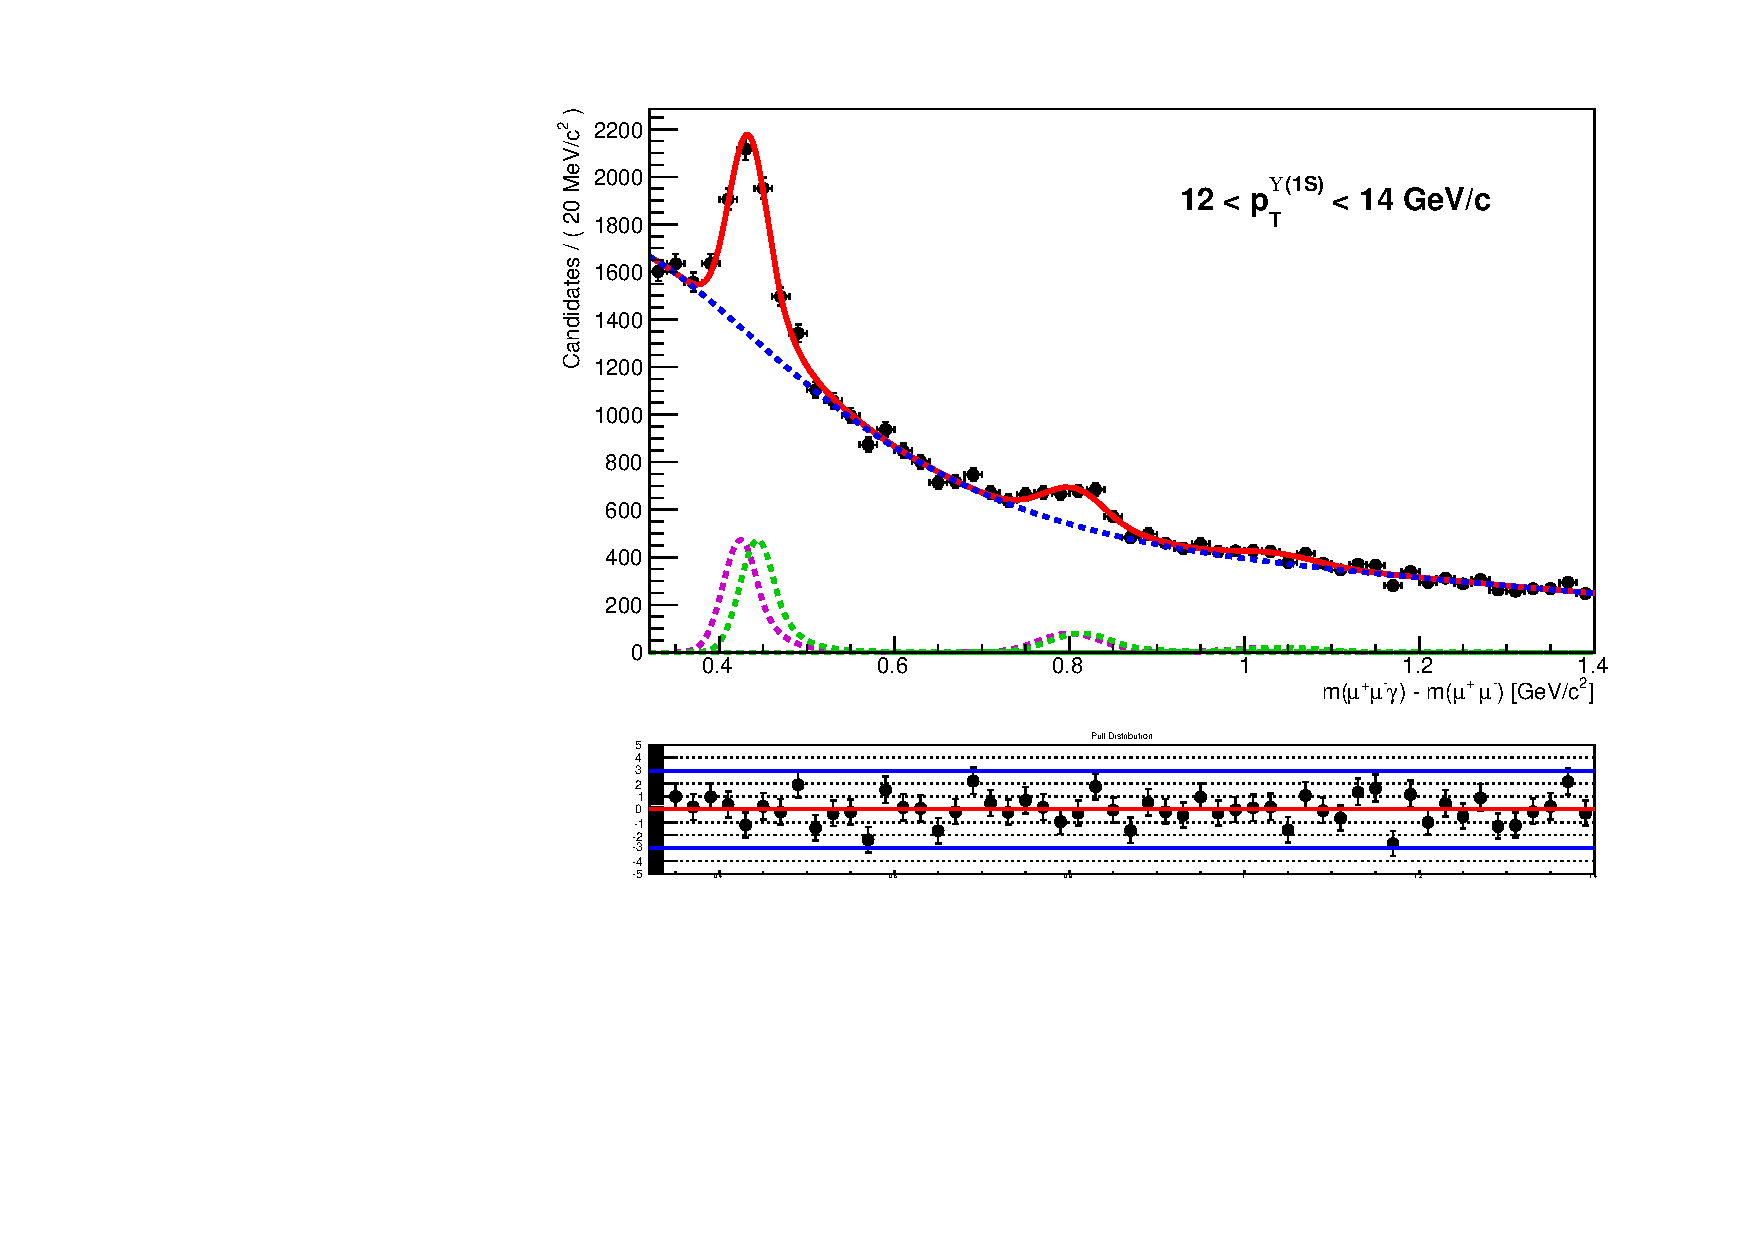
\includegraphics[width=0.31\linewidth]{chib_fits/fit_chib_2012_12_14}
      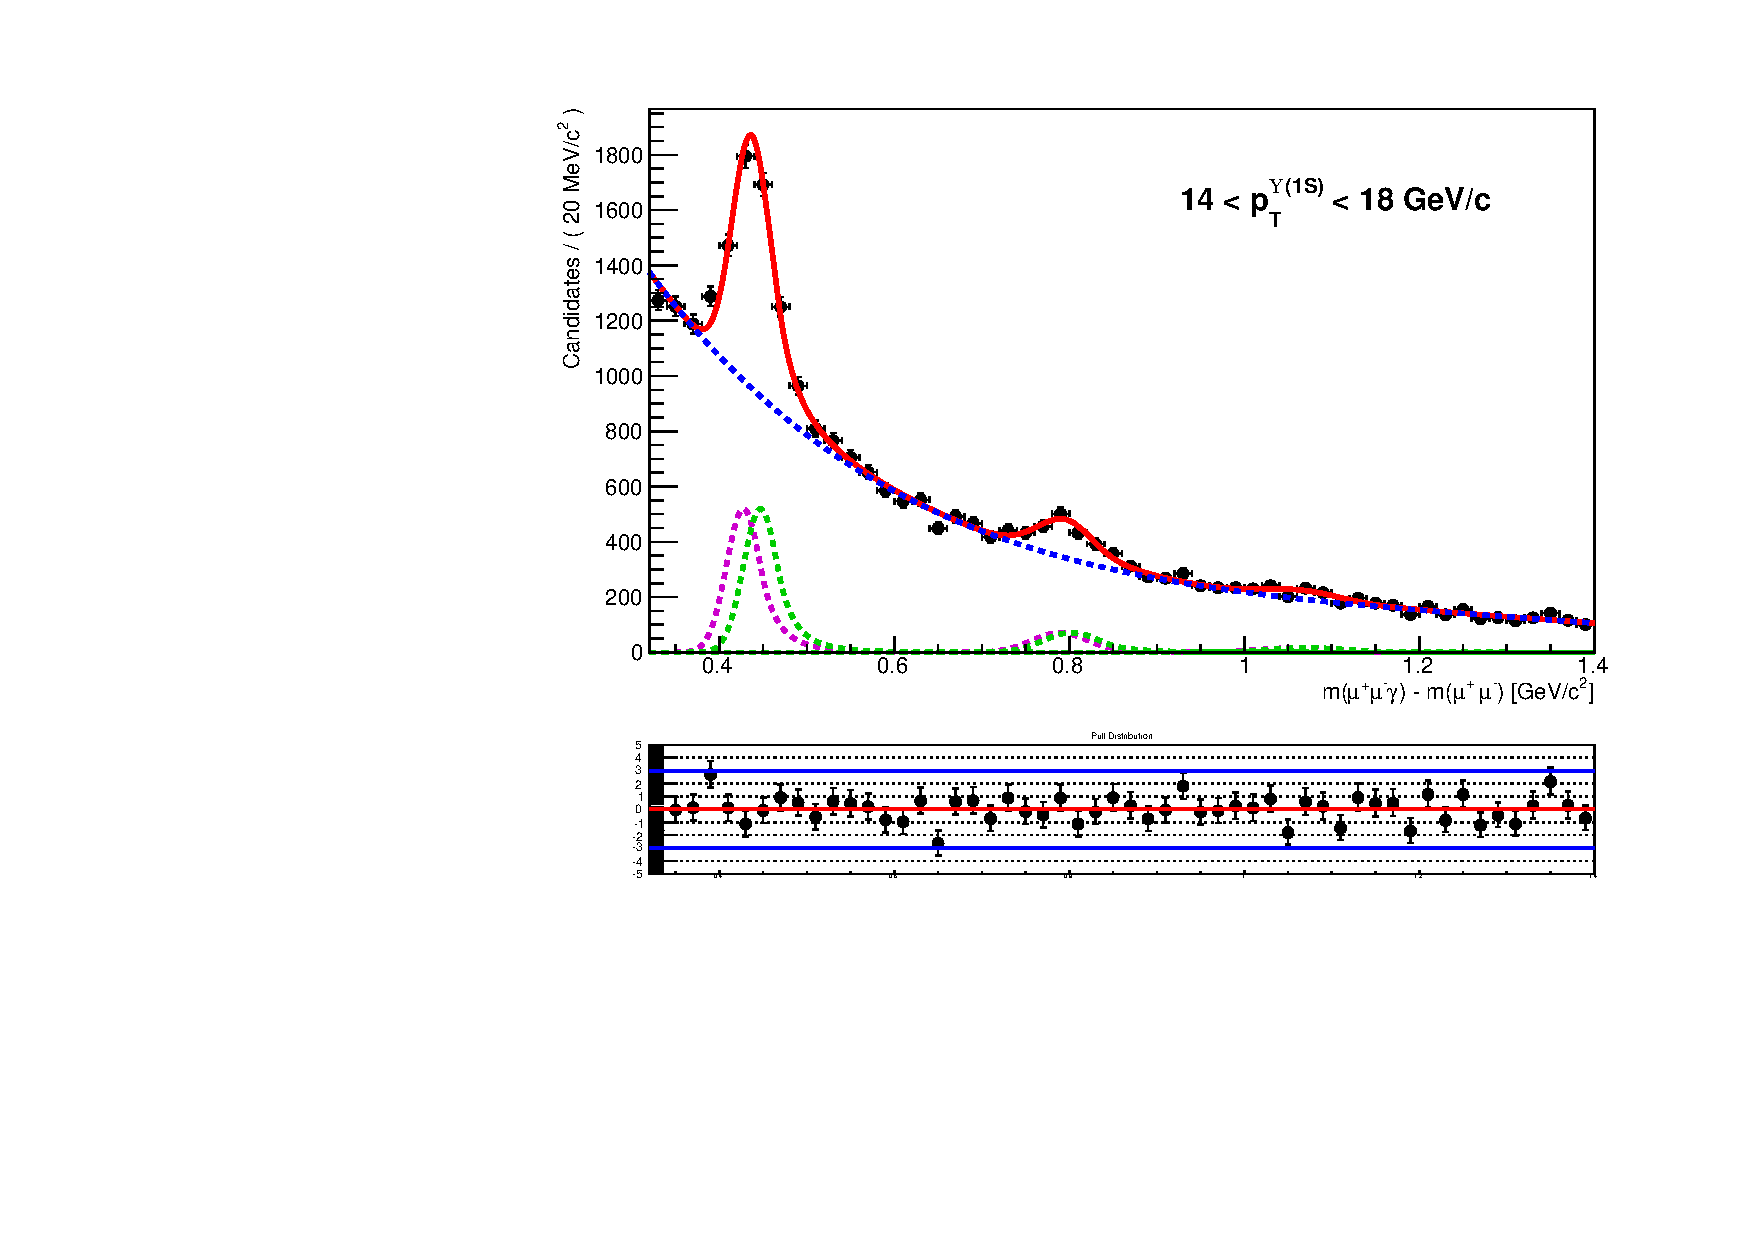
\includegraphics[width=0.31\linewidth]{chib_fits/fit_chib_2012_14_18}
      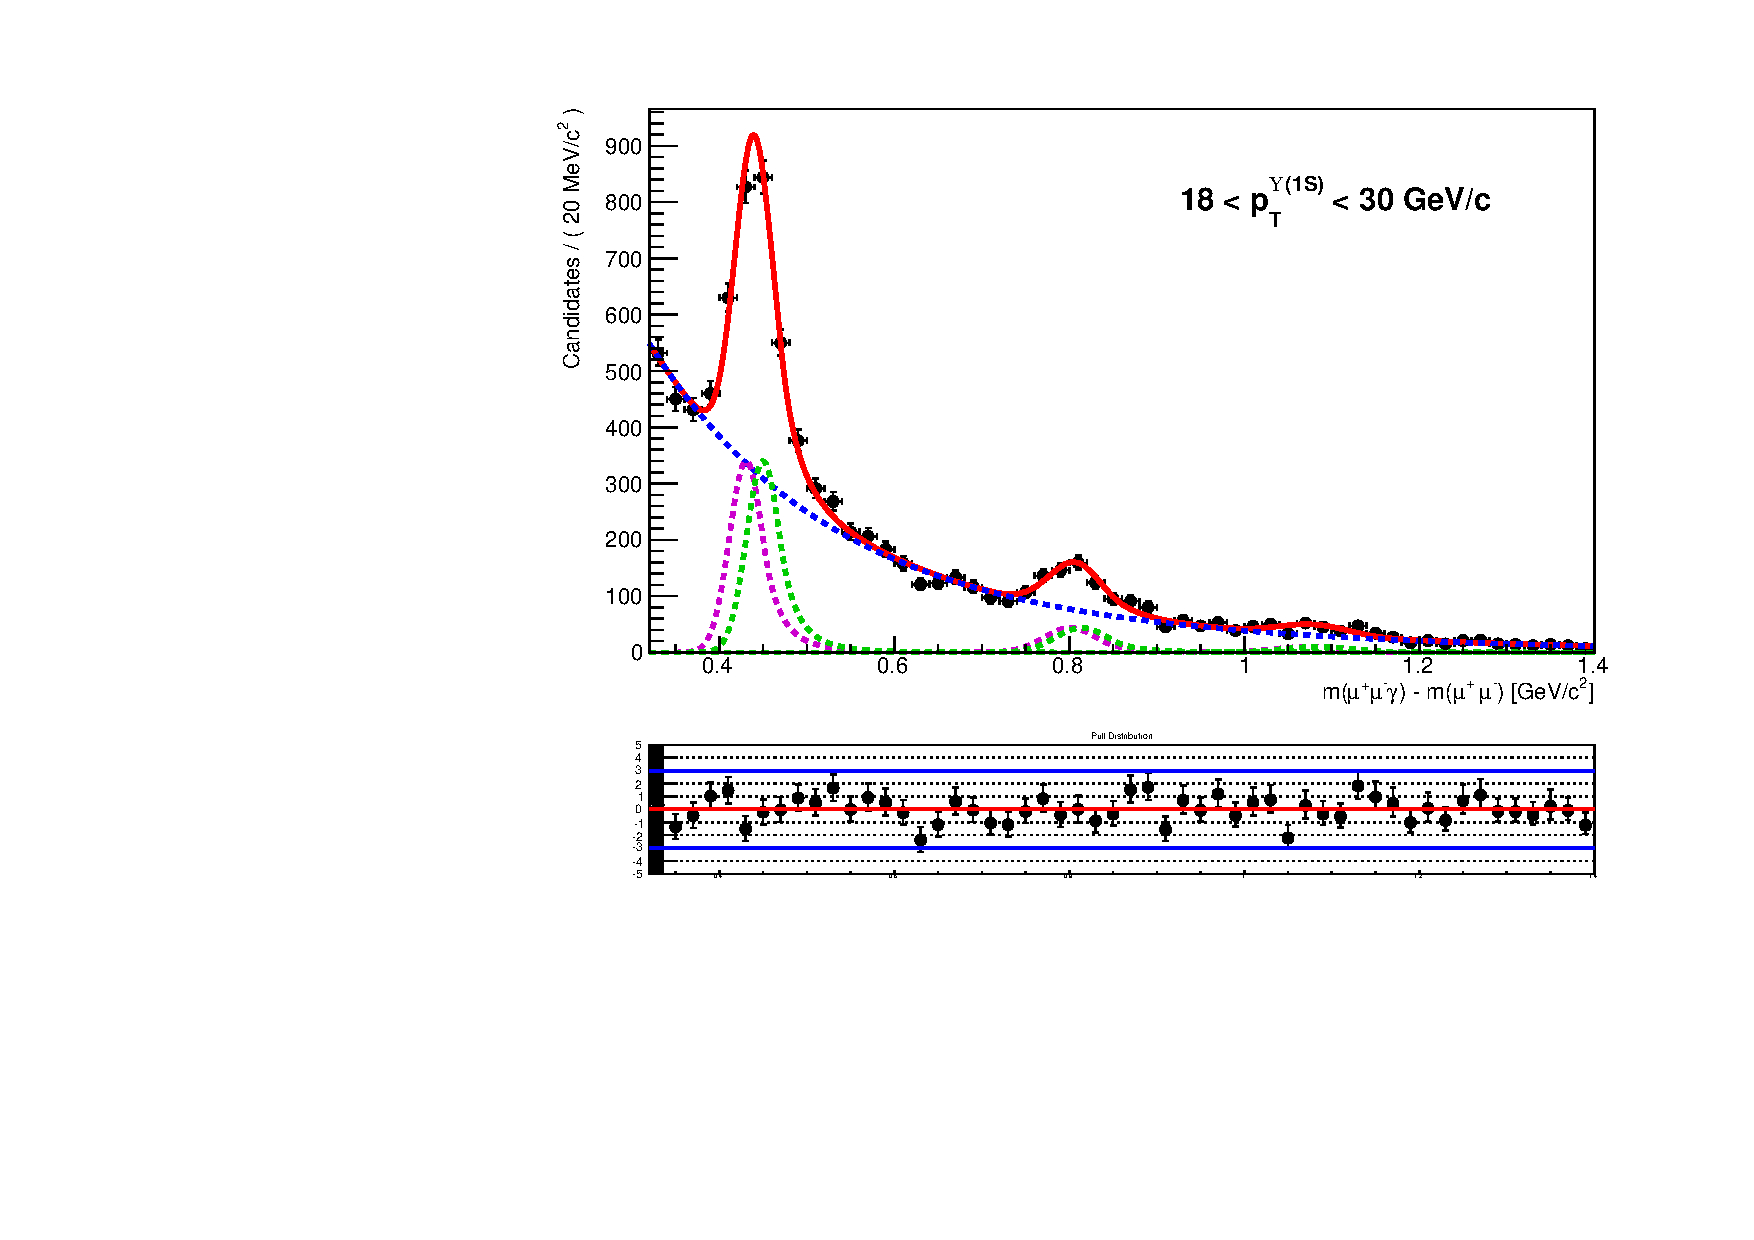
\includegraphics[width=0.31\linewidth]{chib_fits/fit_chib_2012_18_30}
      \caption{\sqs=8\tev (2012)}
      \label{fig:chib_fits_2012}
    \end{subfigure}
  \caption{
    \small  Mass difference of the $\mumu \gamma$ system and $\mumu$ system for the 
    data for specified interval of transverse momentum of the \OneS. The red
    solid line is the result of the fit described in the text. Blue dashed line 
    is the background contribution obtained from the fit. Magenta and green 
    dashed lines are \chibone and \chibtwo signal contribution obtained from the fit.
  }
  \label{fig:chib_fits}
\end{figure}


\begin{figure}[ht]
  \centering
    \begin{subfigure}[b]{\textwidth}
      \centering
      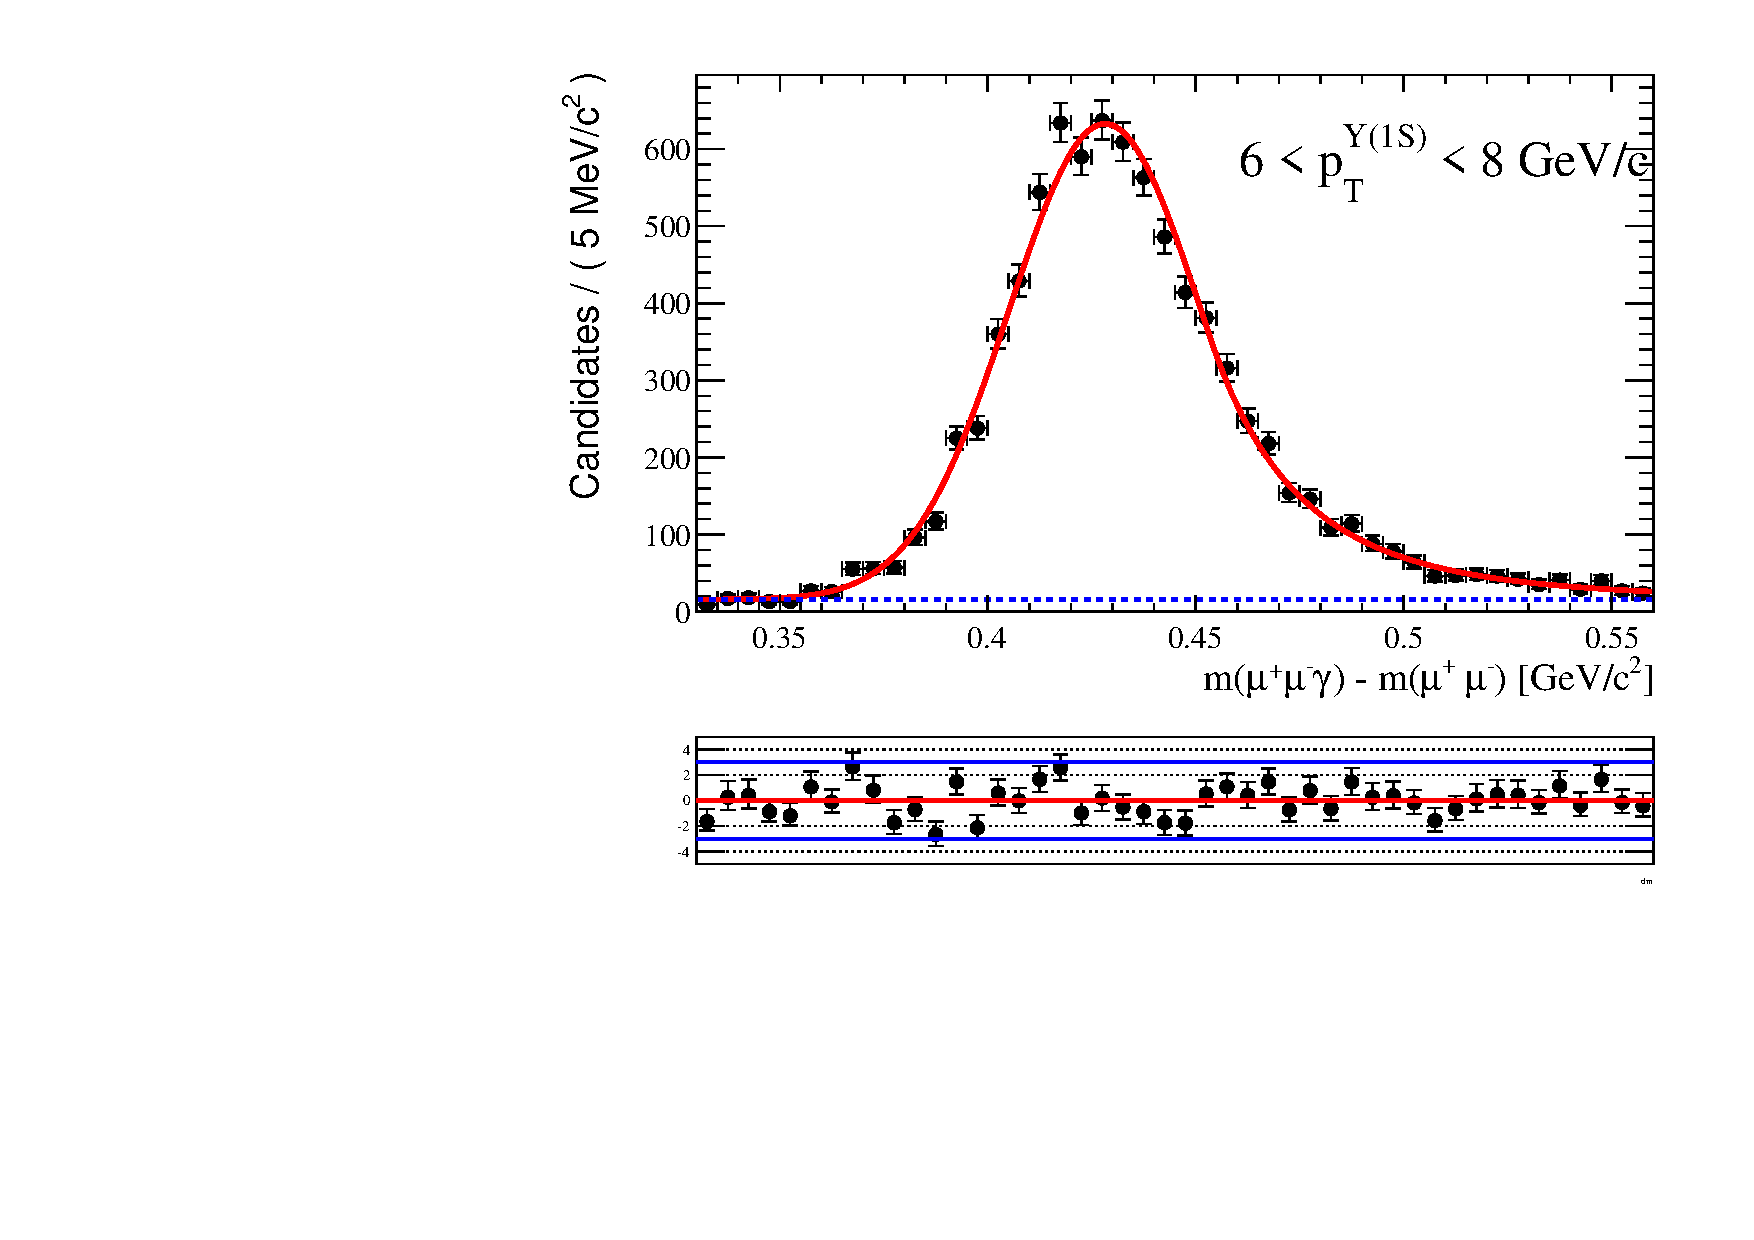
\includegraphics[width=0.16\linewidth]{fit_mc/chib11_6_8}
      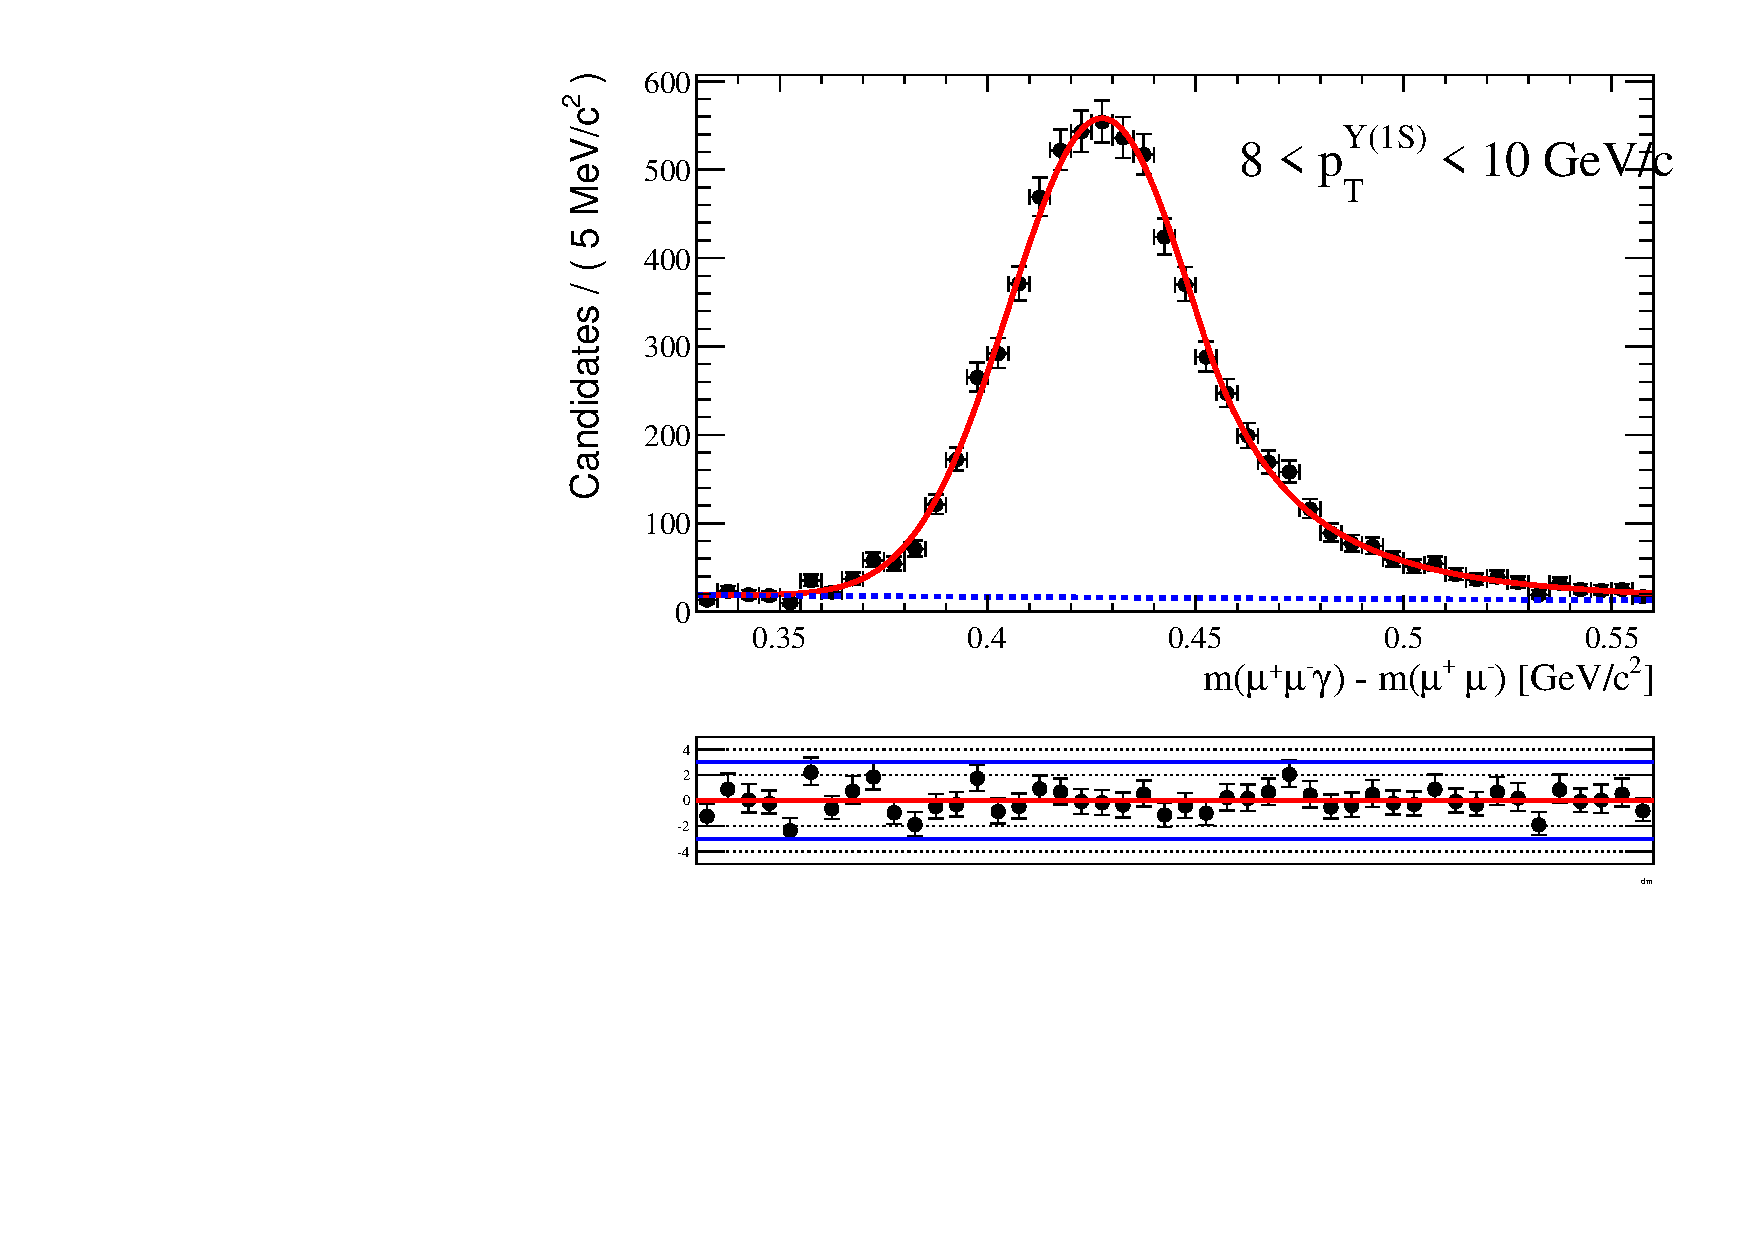
\includegraphics[width=0.16\linewidth]{fit_mc/chib11_8_10}
      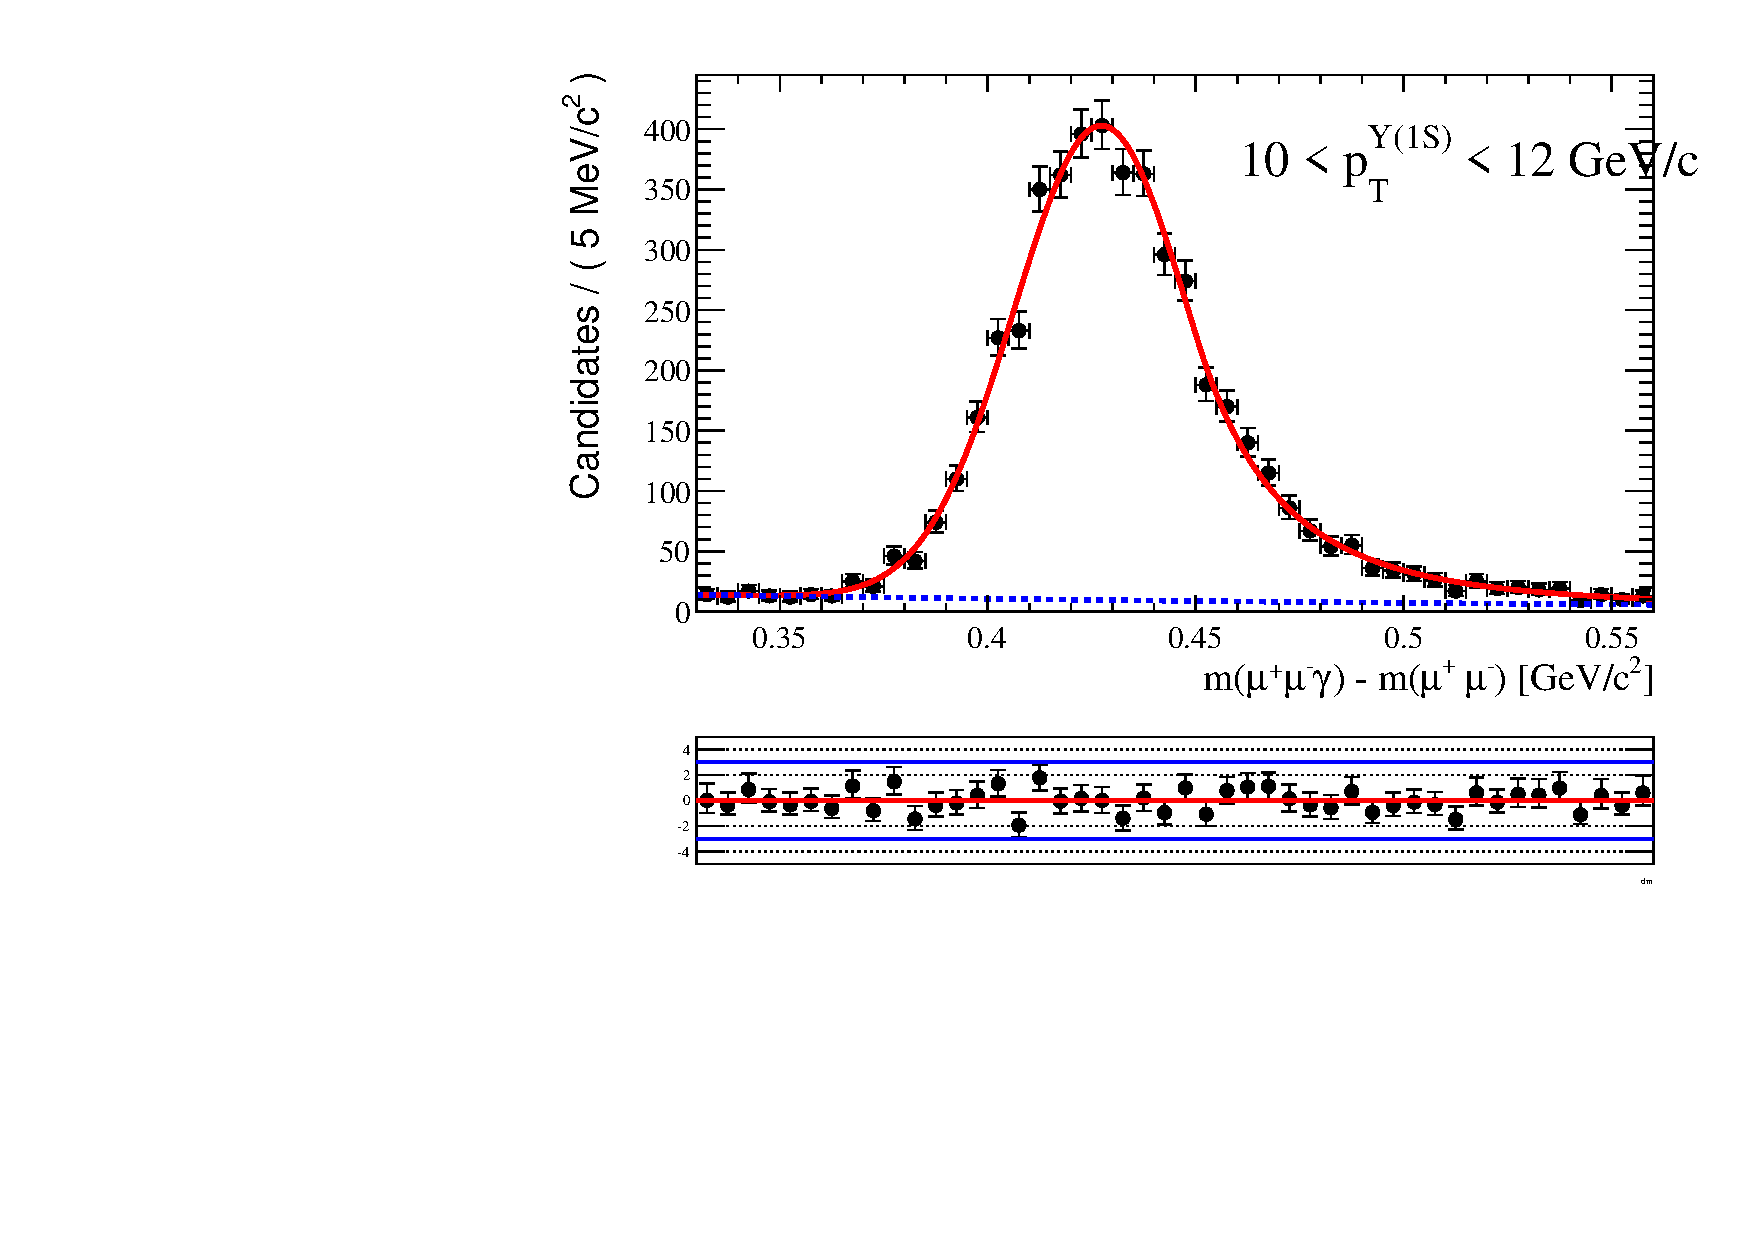
\includegraphics[width=0.16\linewidth]{fit_mc/chib11_10_12}
      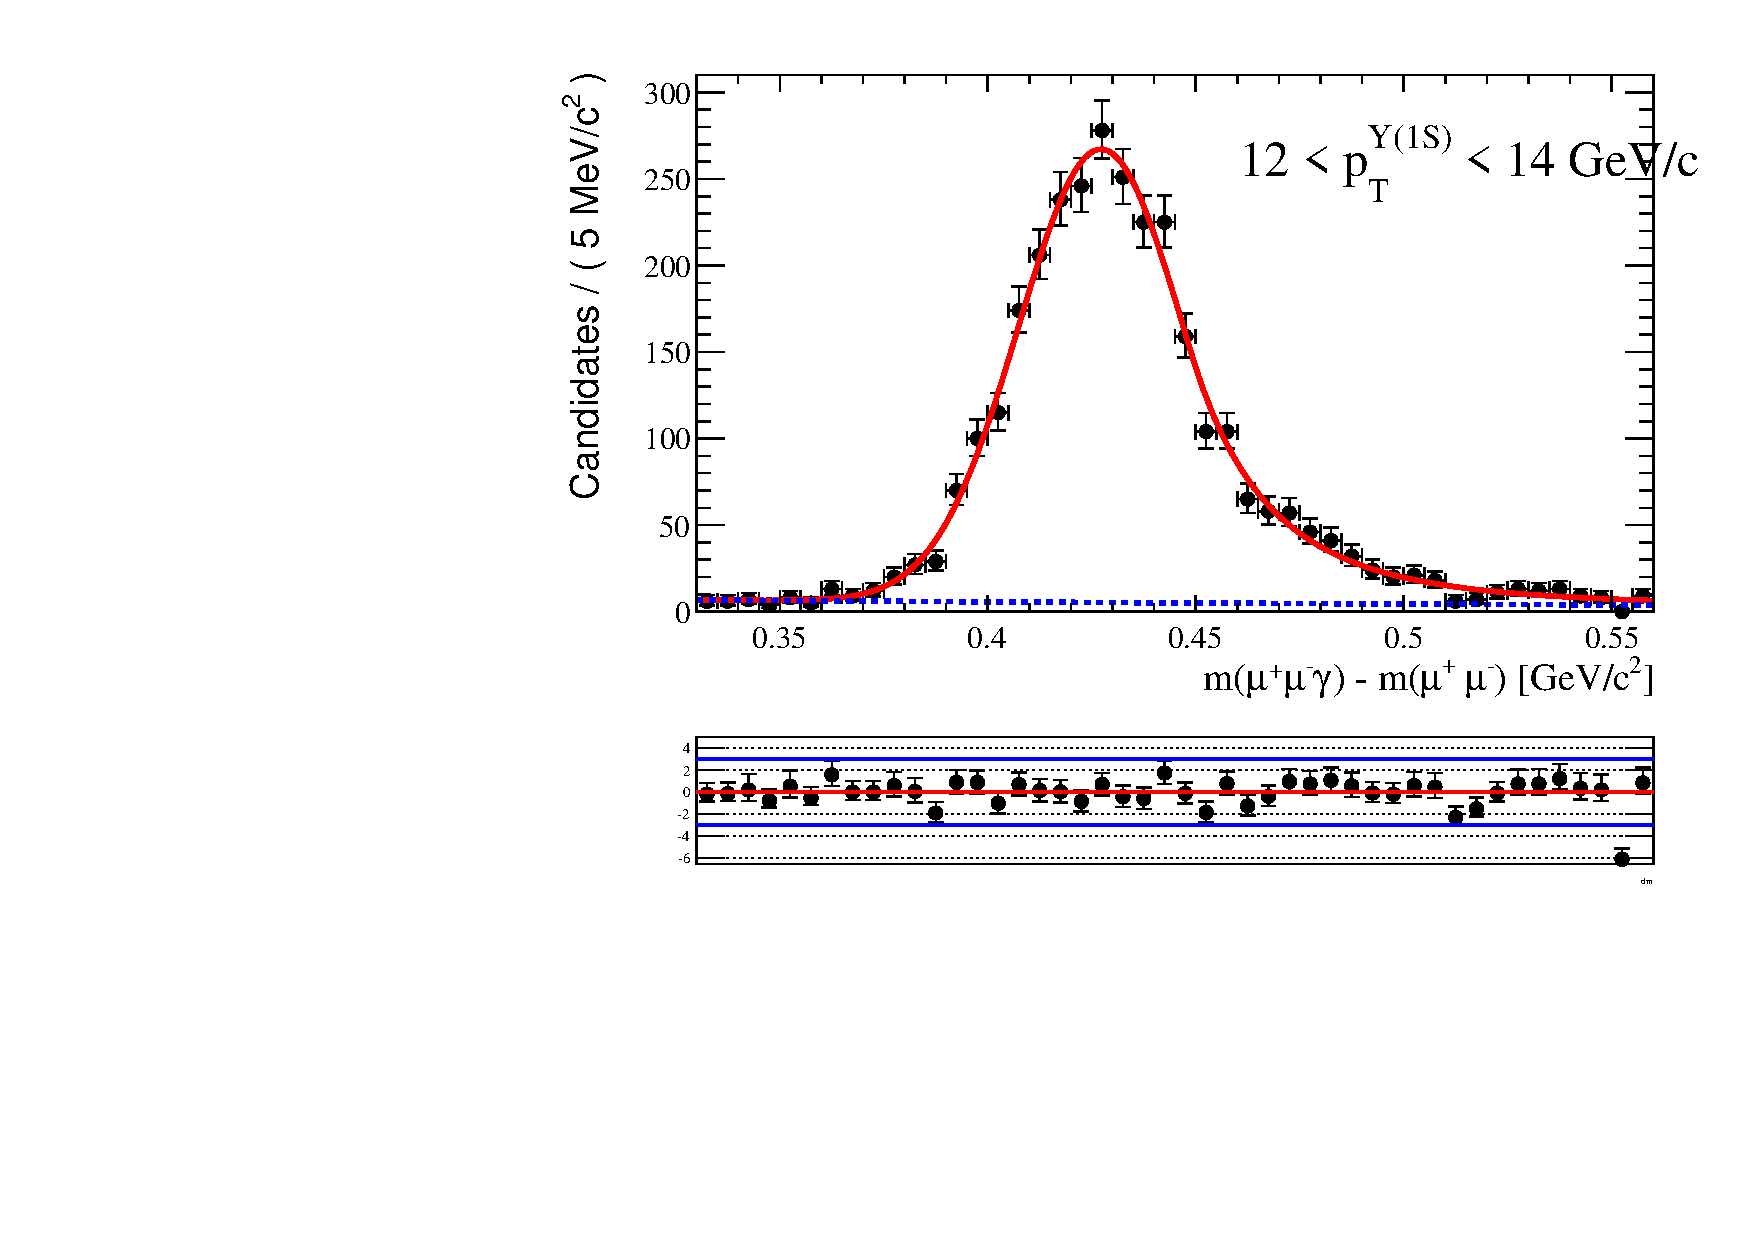
\includegraphics[width=0.16\linewidth]{fit_mc/chib11_12_14}
      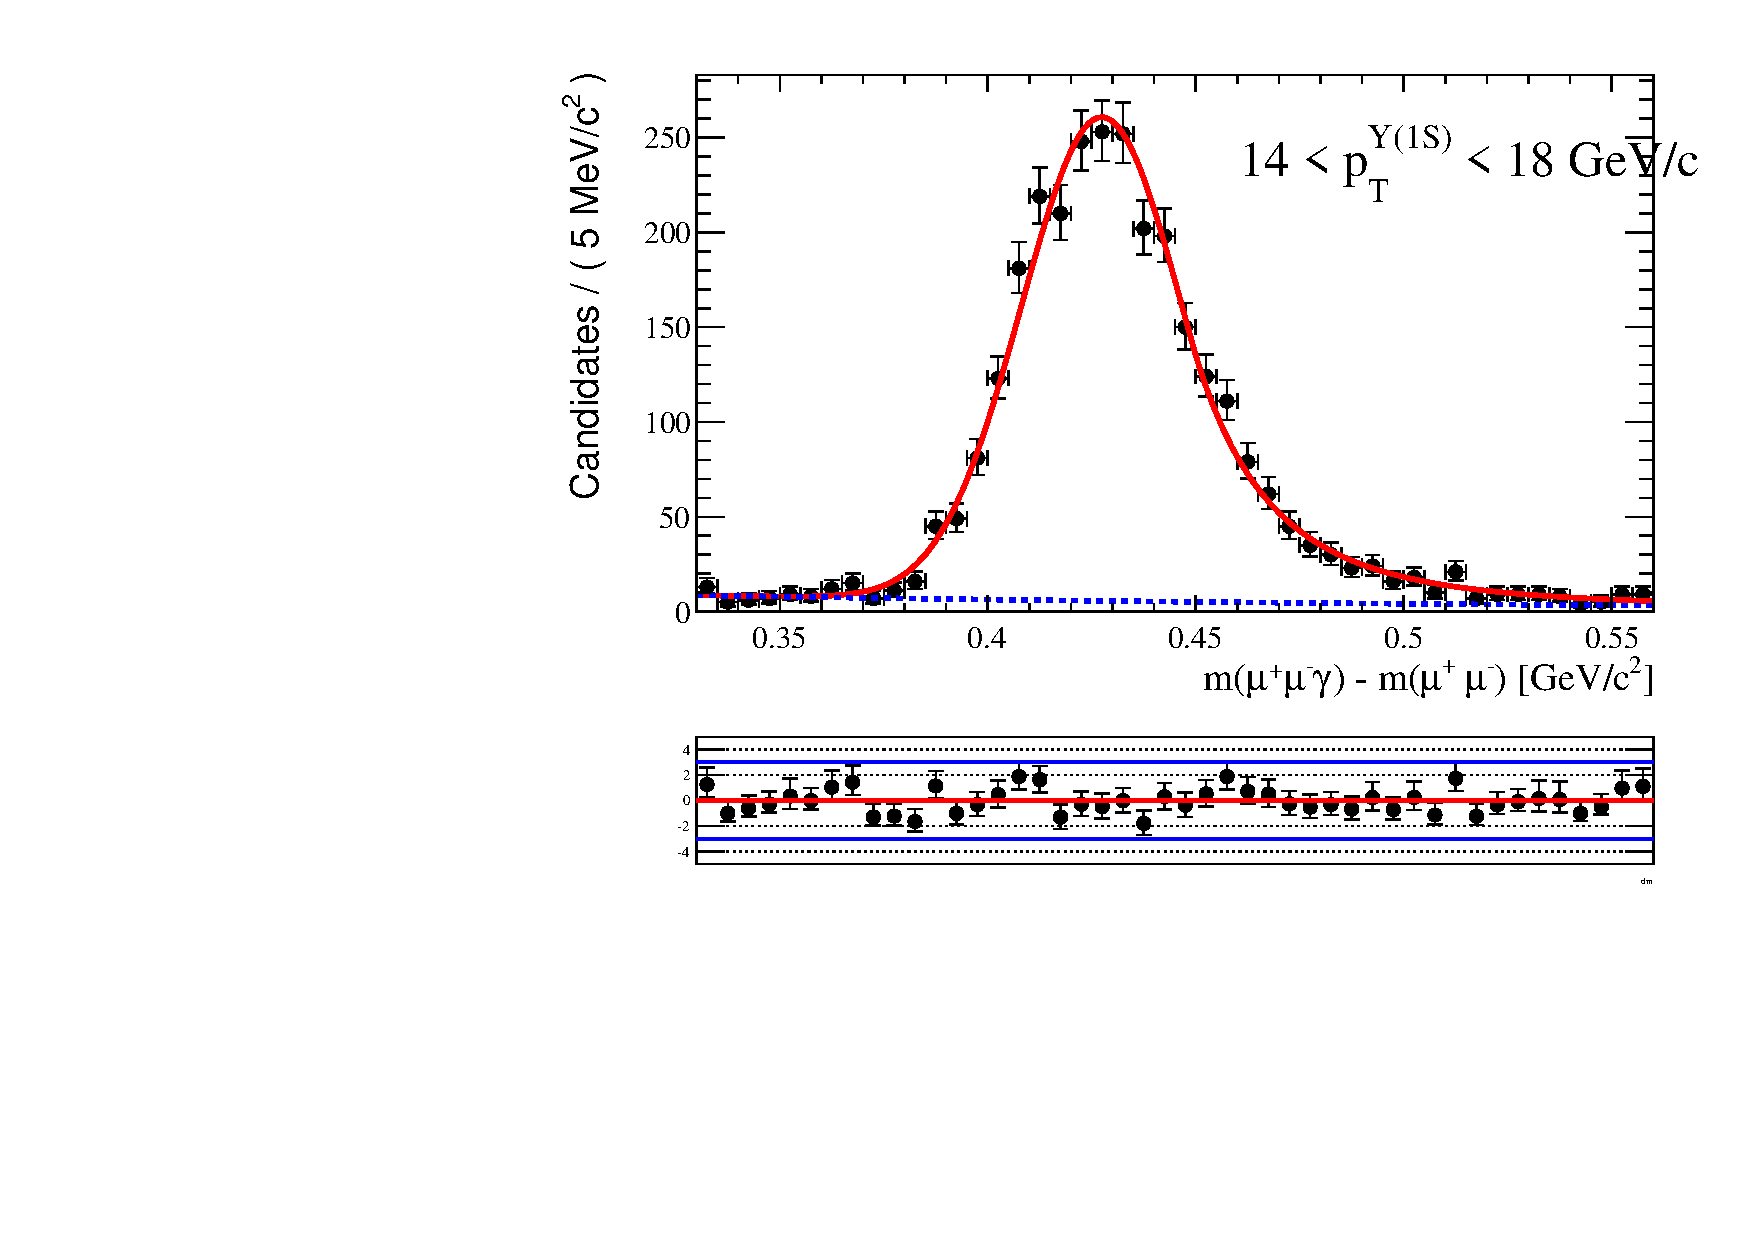
\includegraphics[width=0.16\linewidth]{fit_mc/chib11_14_18}
      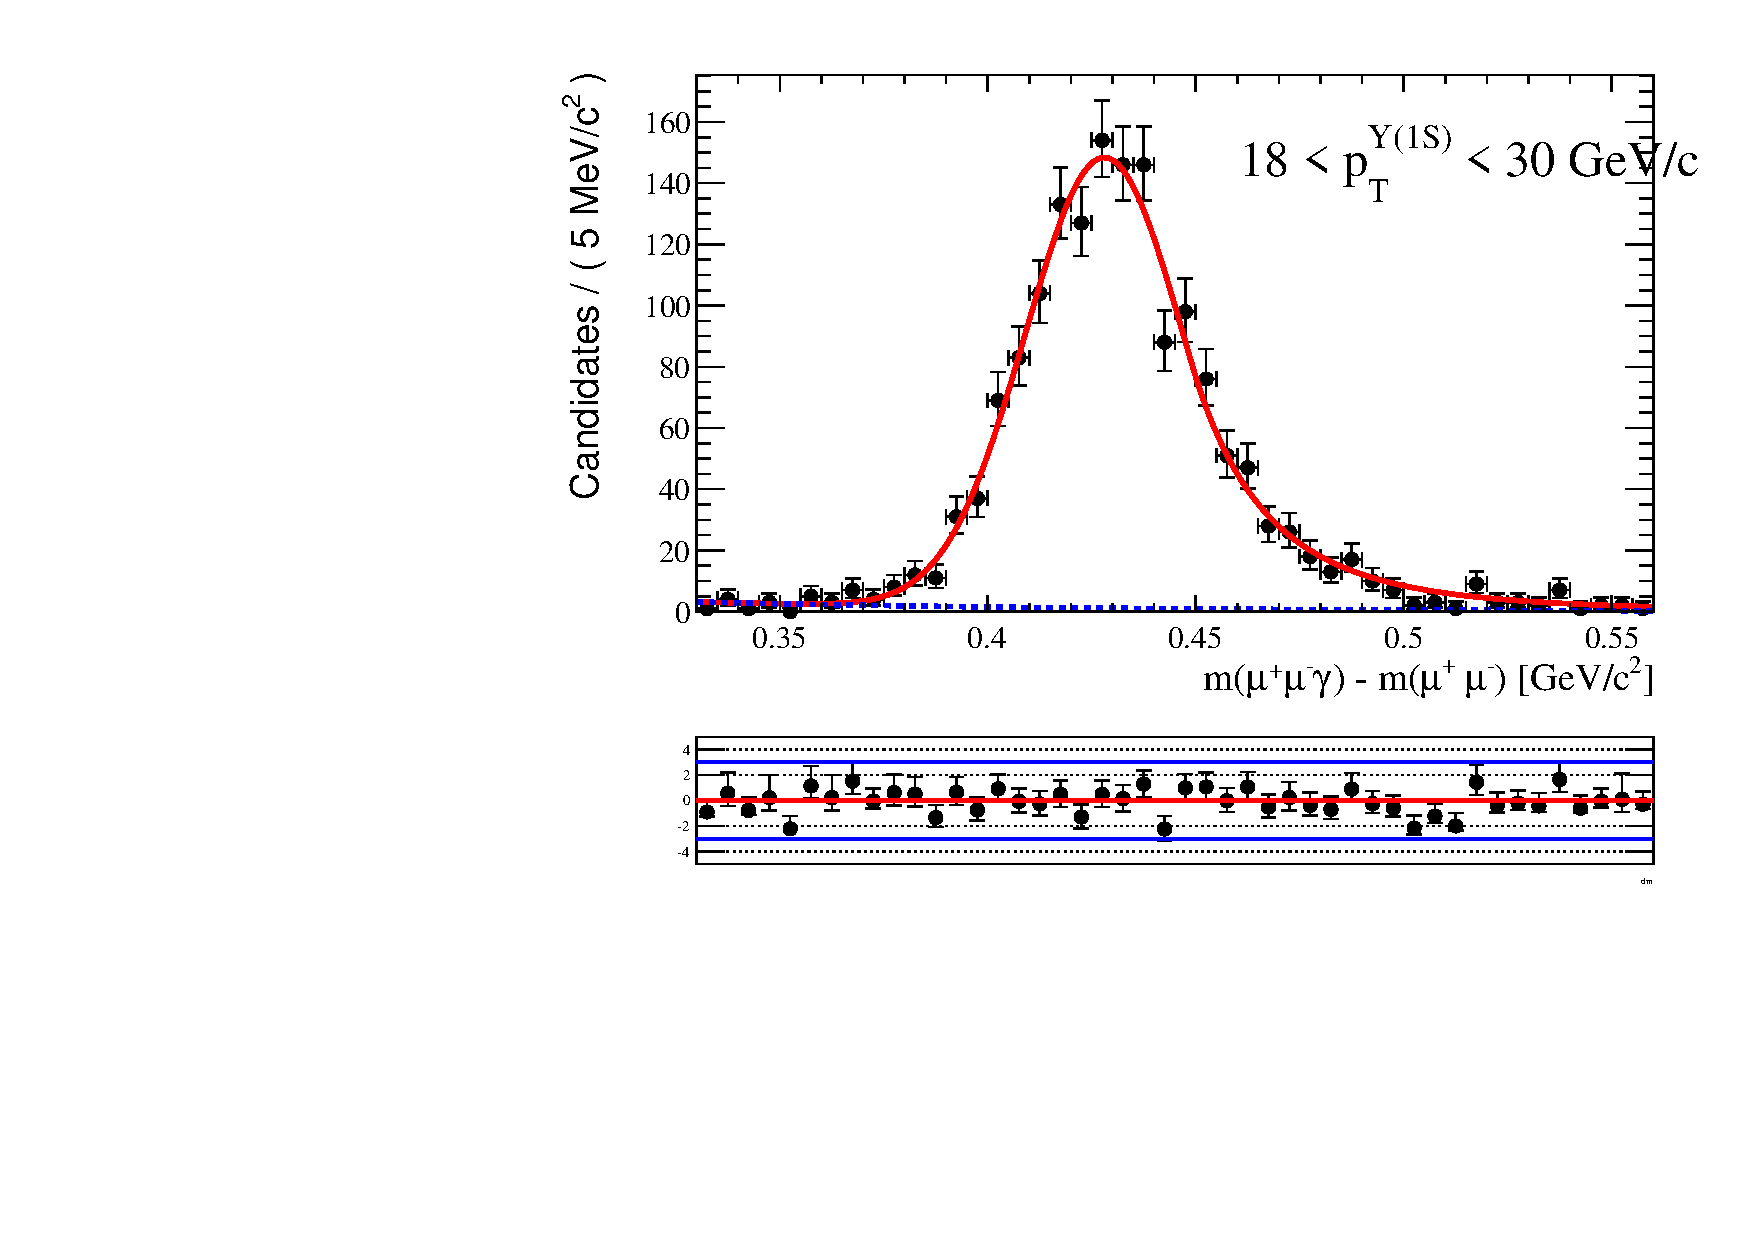
\includegraphics[width=0.16\linewidth]{fit_mc/chib11_18_30}
      \caption{\chiboneOneP}
      \label{fig:fit_mc_chiboneOneP}
    \end{subfigure}
    \begin{subfigure}[b]{\textwidth}
      \centering
      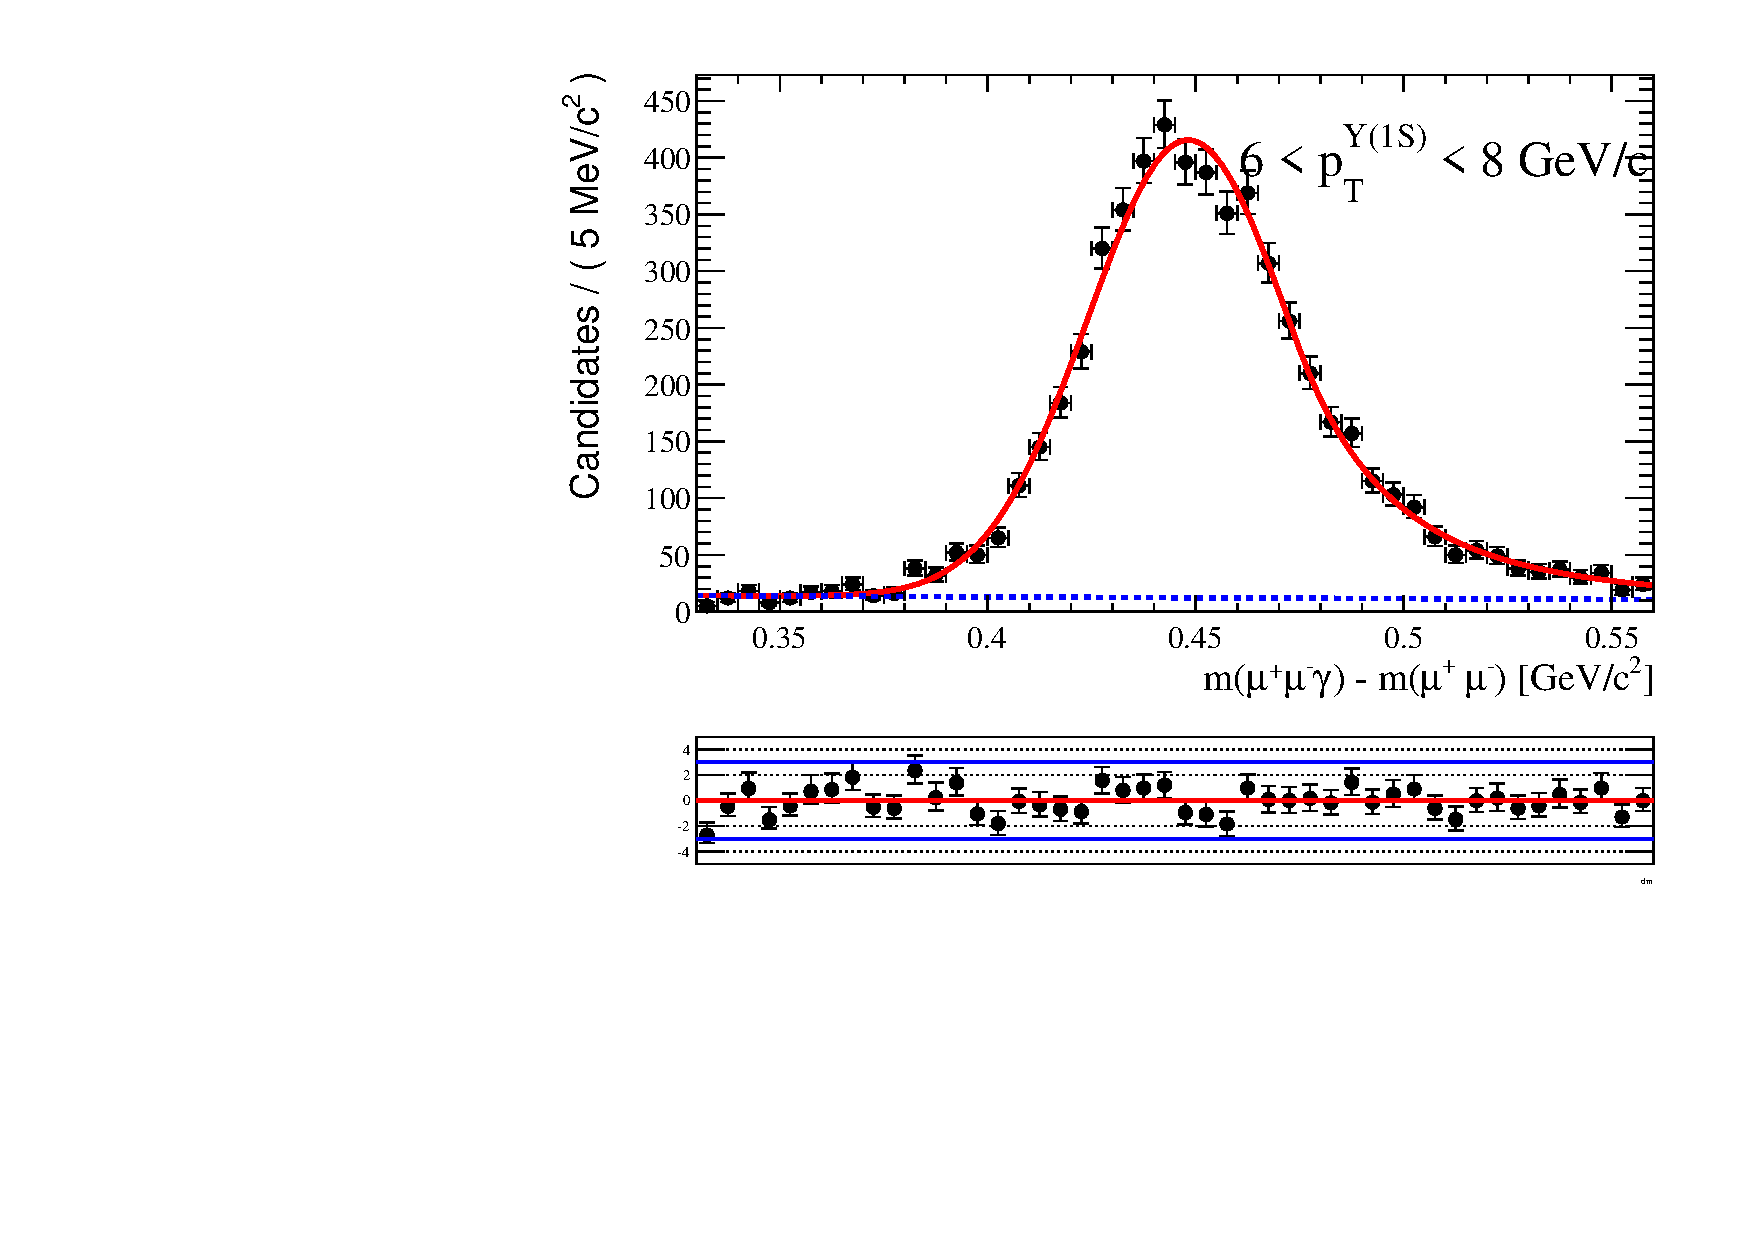
\includegraphics[width=0.16\linewidth]{fit_mc/chib21_6_8}
      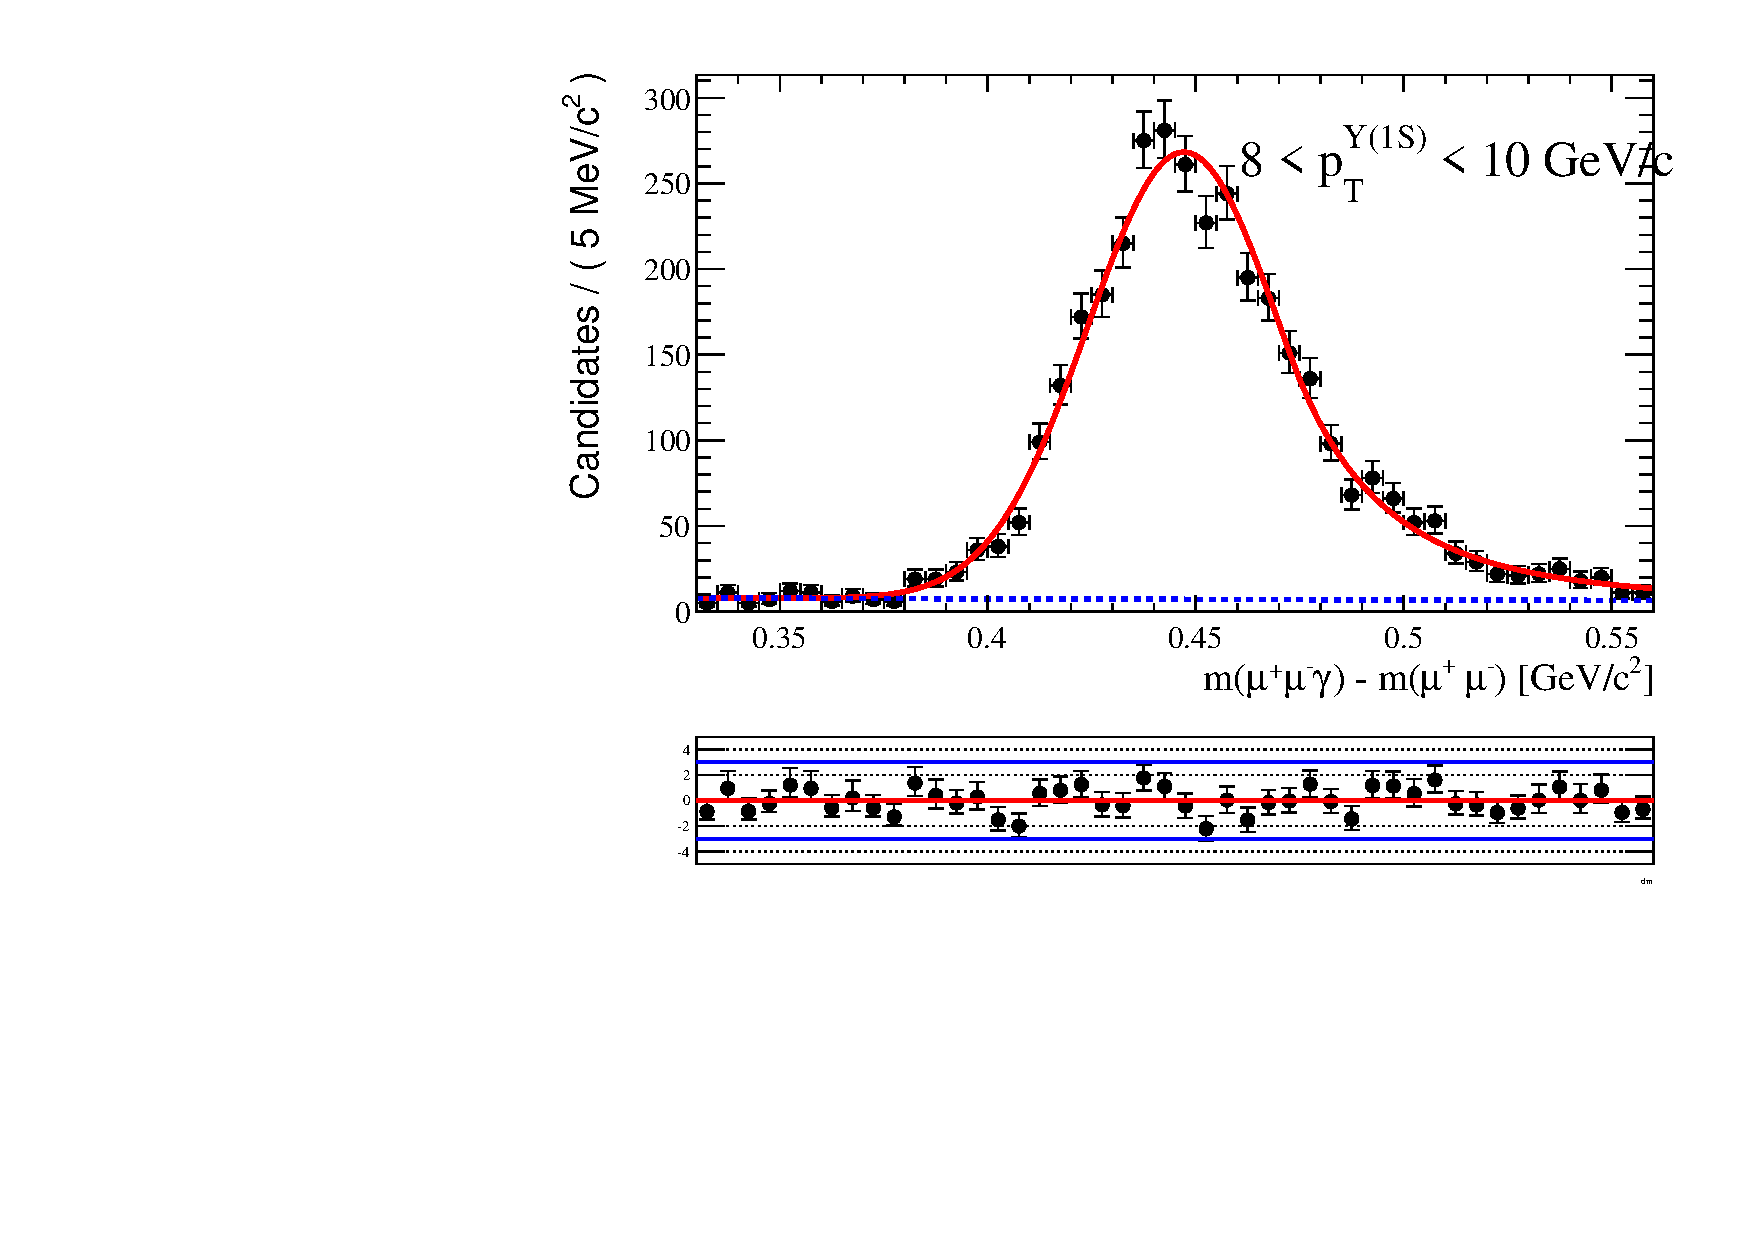
\includegraphics[width=0.16\linewidth]{fit_mc/chib21_8_10}
      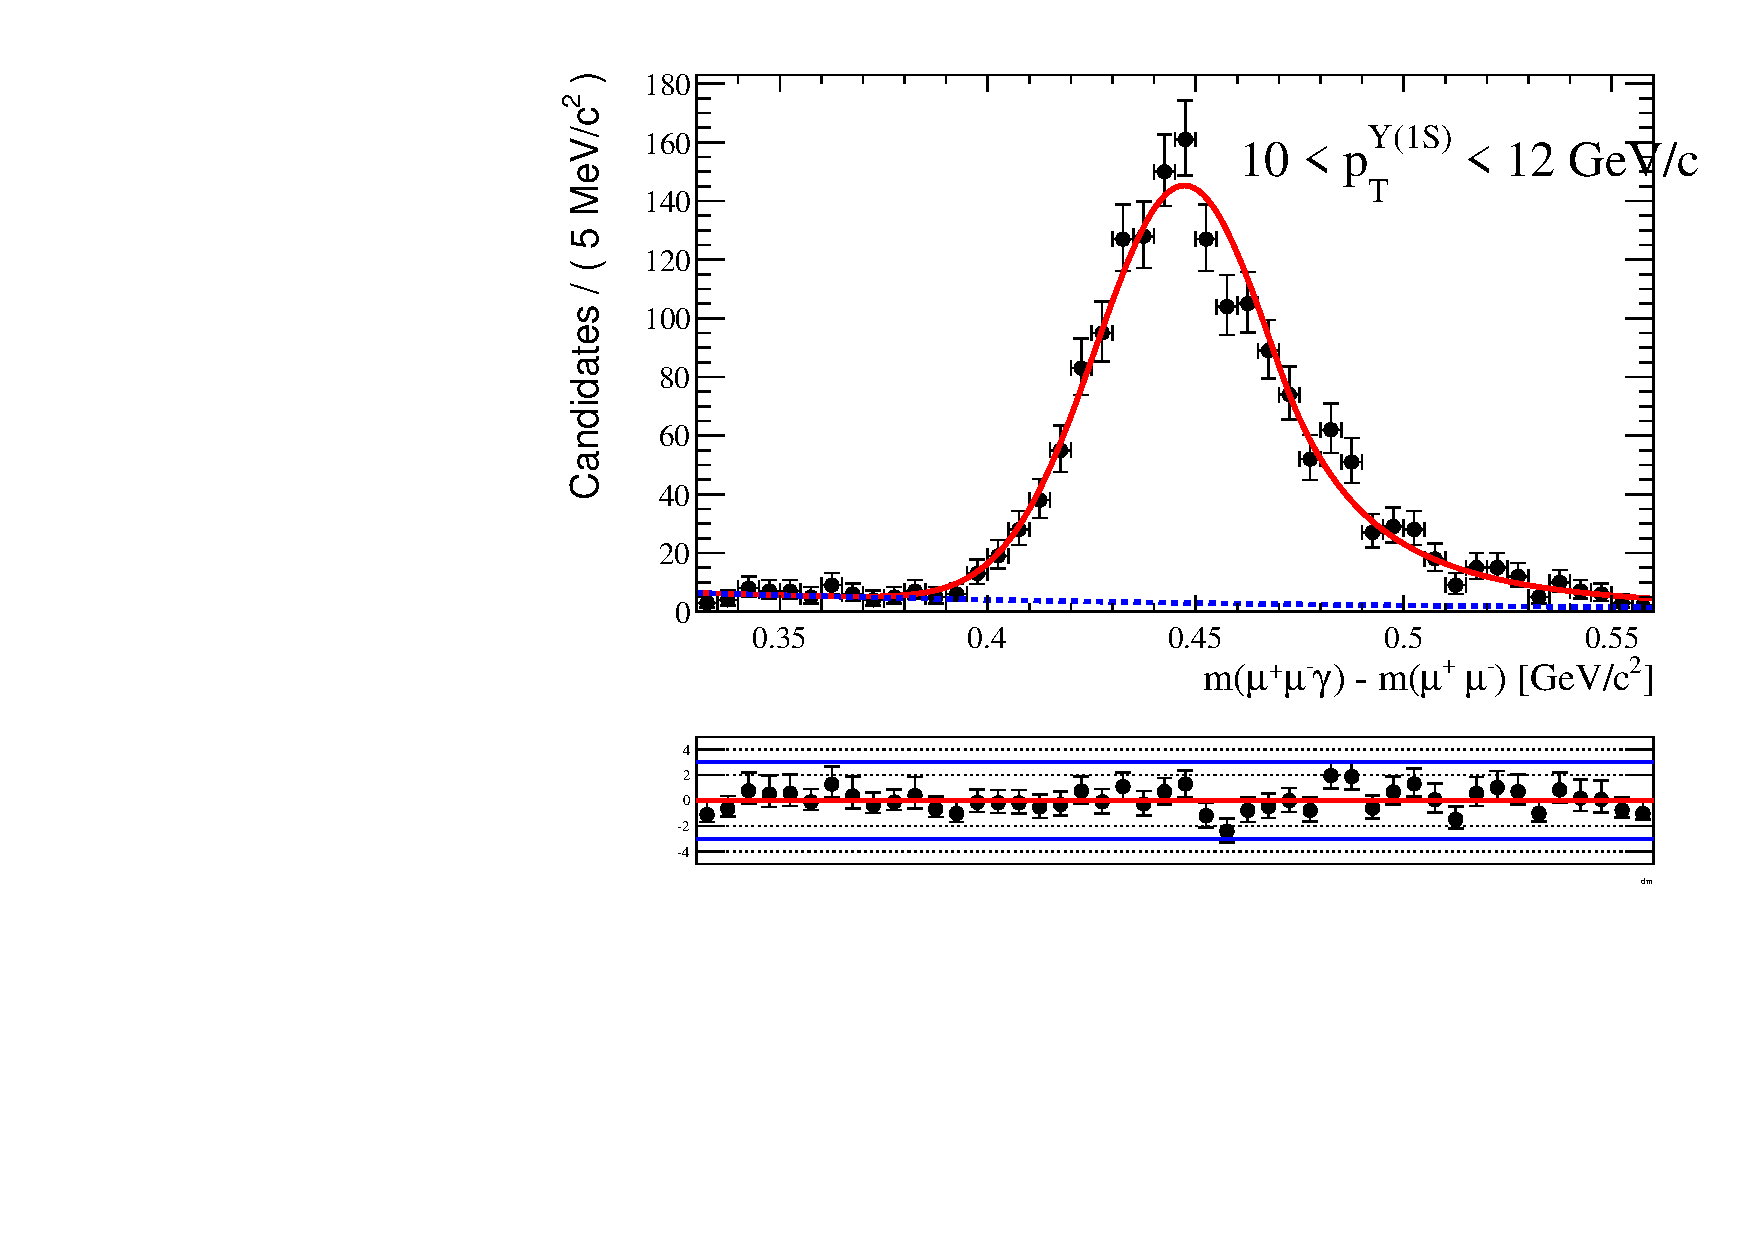
\includegraphics[width=0.16\linewidth]{fit_mc/chib21_10_12}
      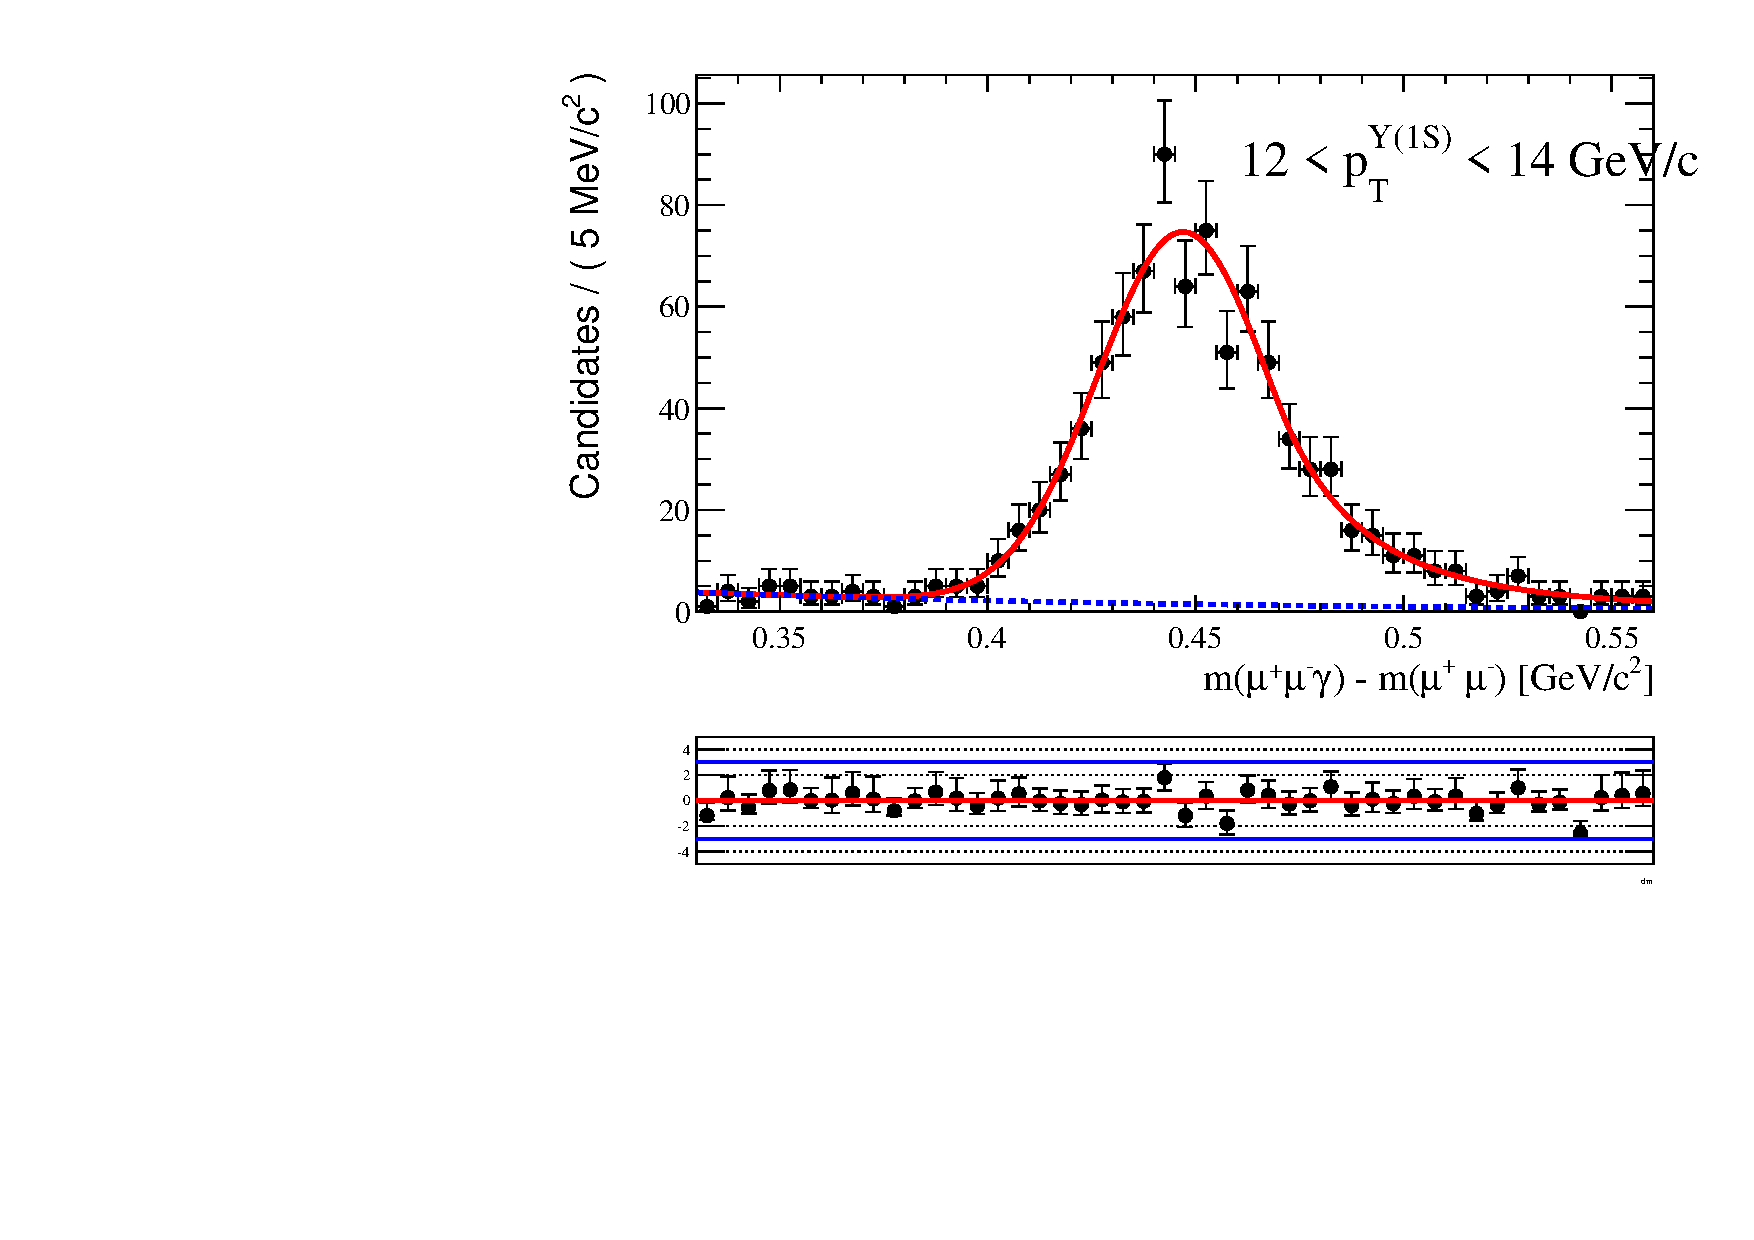
\includegraphics[width=0.16\linewidth]{fit_mc/chib21_12_14}
      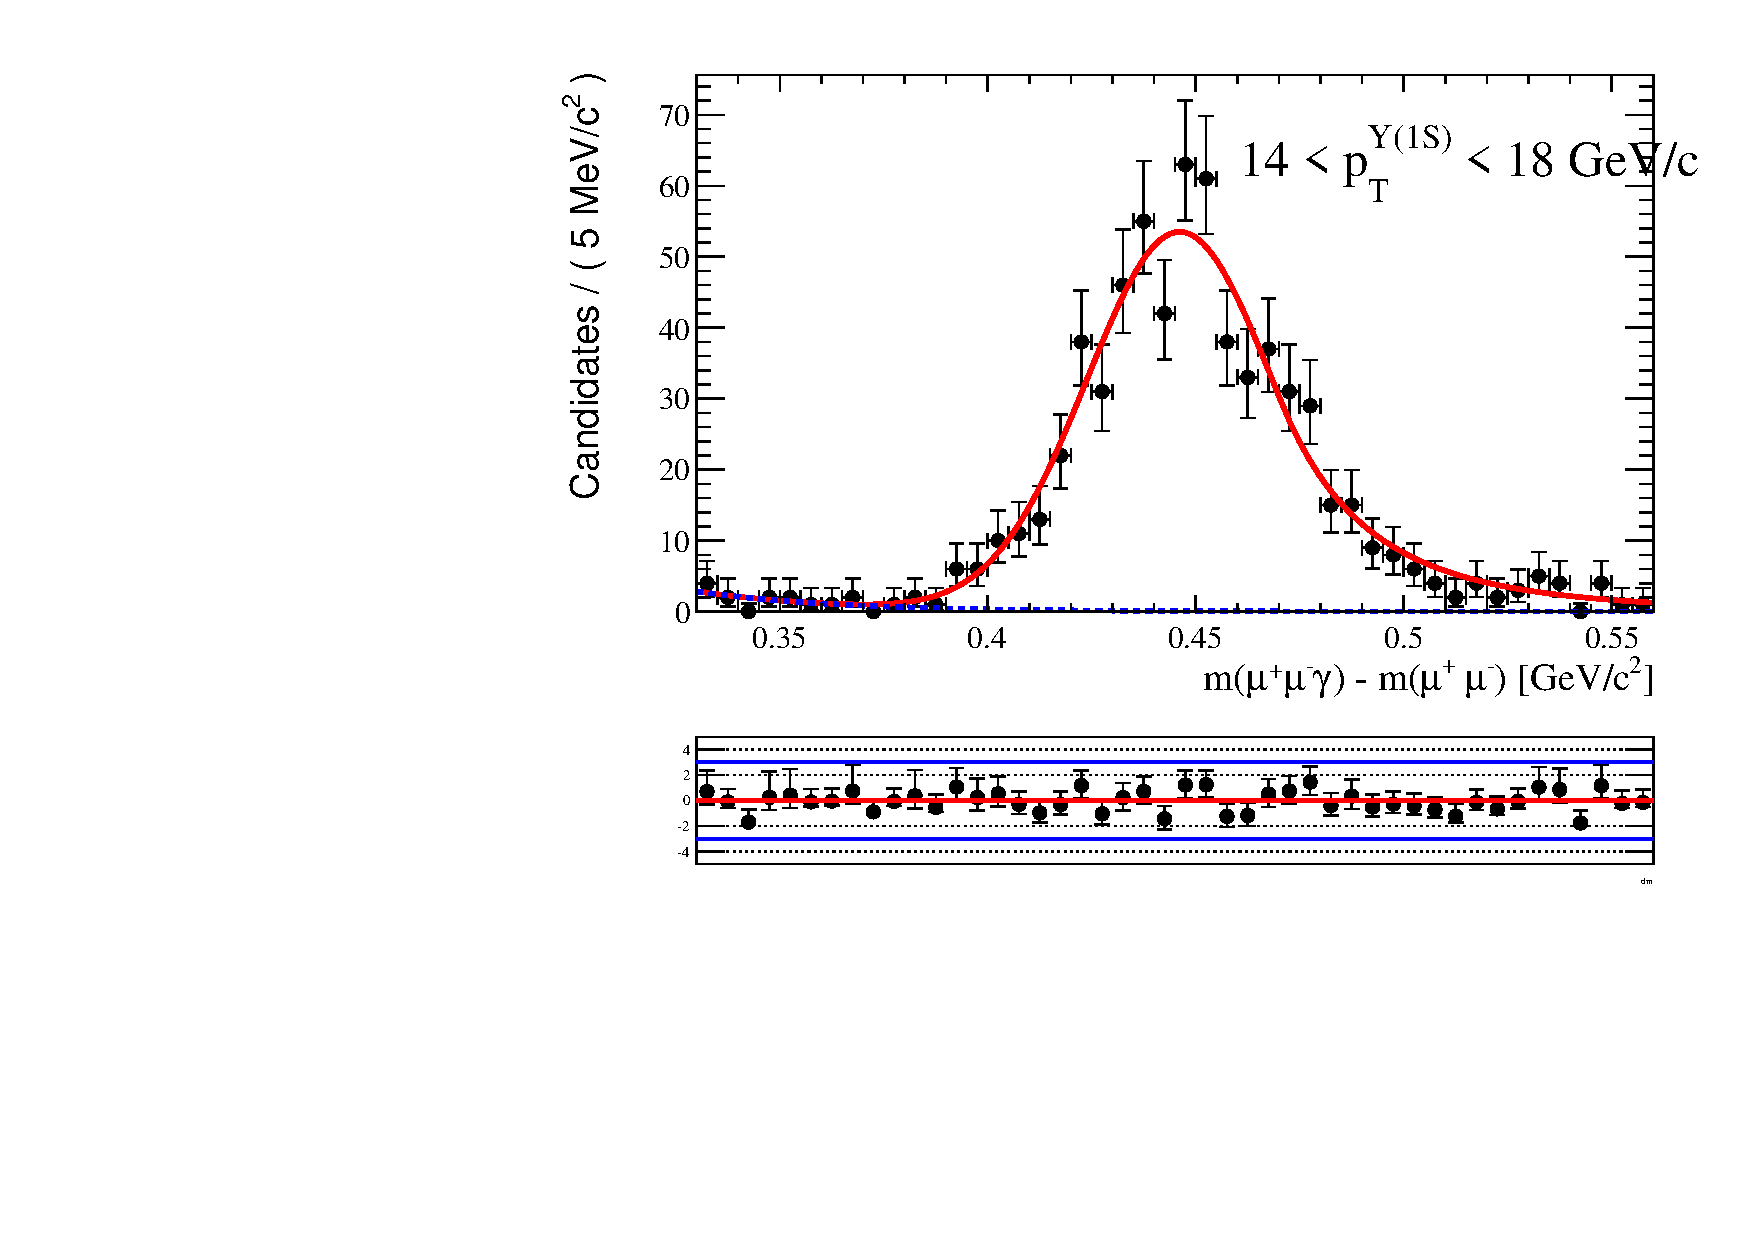
\includegraphics[width=0.16\linewidth]{fit_mc/chib21_14_18}
      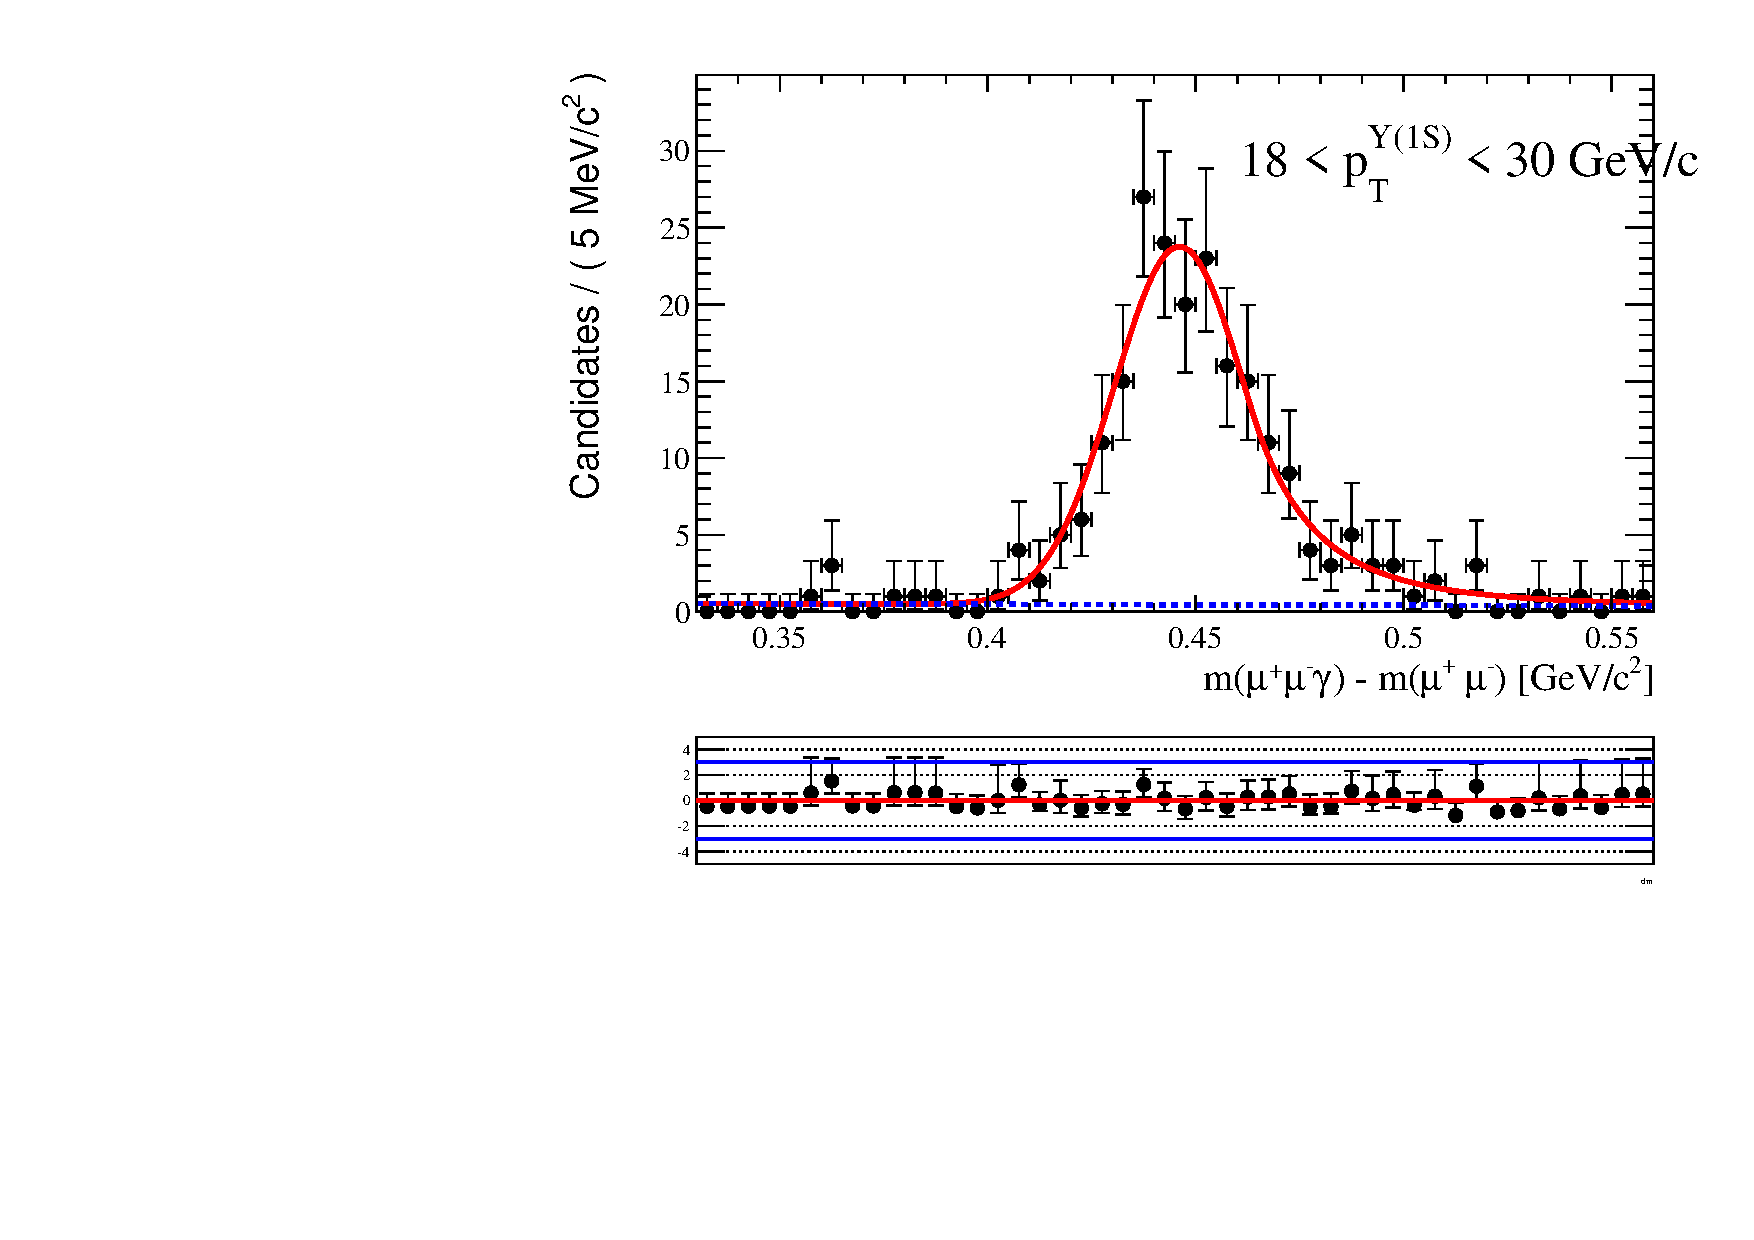
\includegraphics[width=0.16\linewidth]{fit_mc/chib21_18_30}
      \caption{\chibtwoOneP}
      \label{fig:fit_mc_chibtwoOneP}
    \end{subfigure}
    \begin{subfigure}[b]{\textwidth}
      \centering
      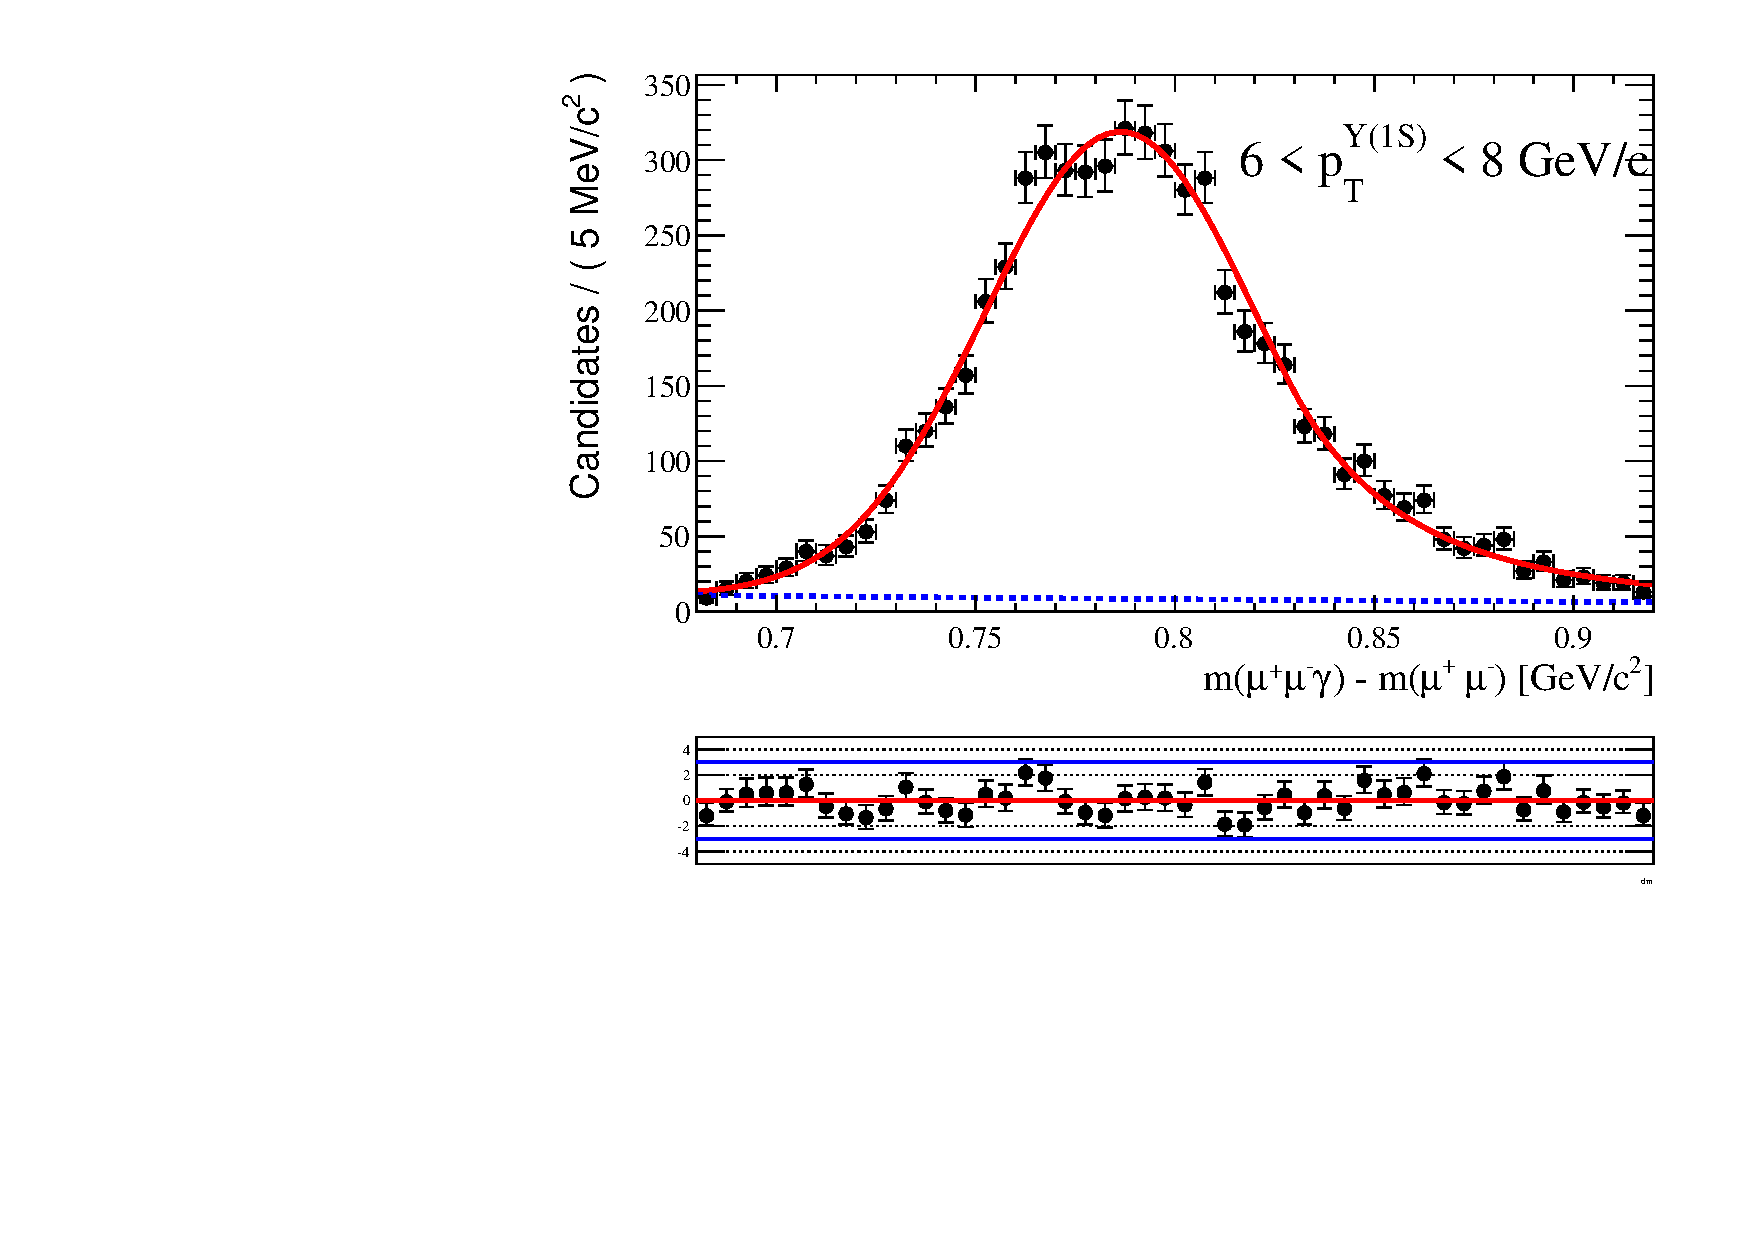
\includegraphics[width=0.16\linewidth]{fit_mc/chib12_6_8}
      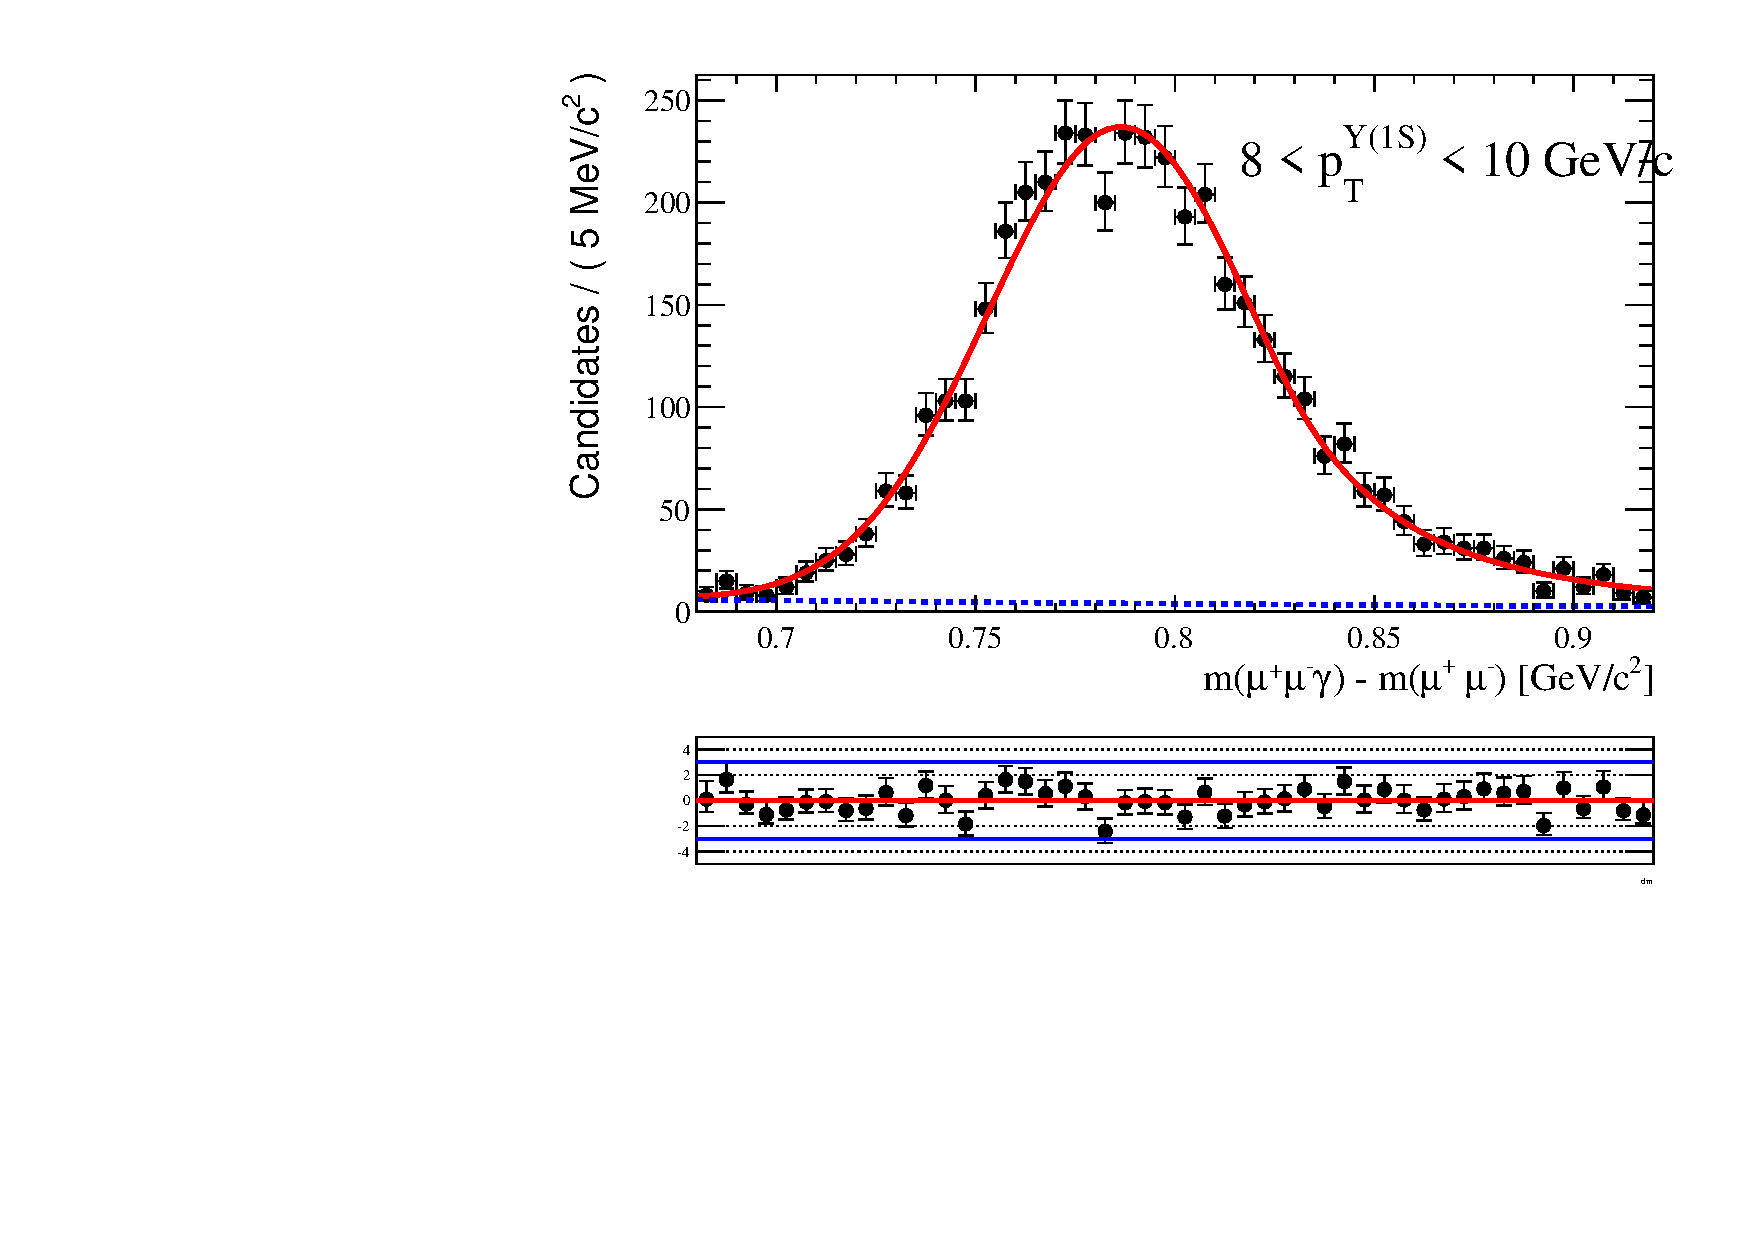
\includegraphics[width=0.16\linewidth]{fit_mc/chib12_8_10}
      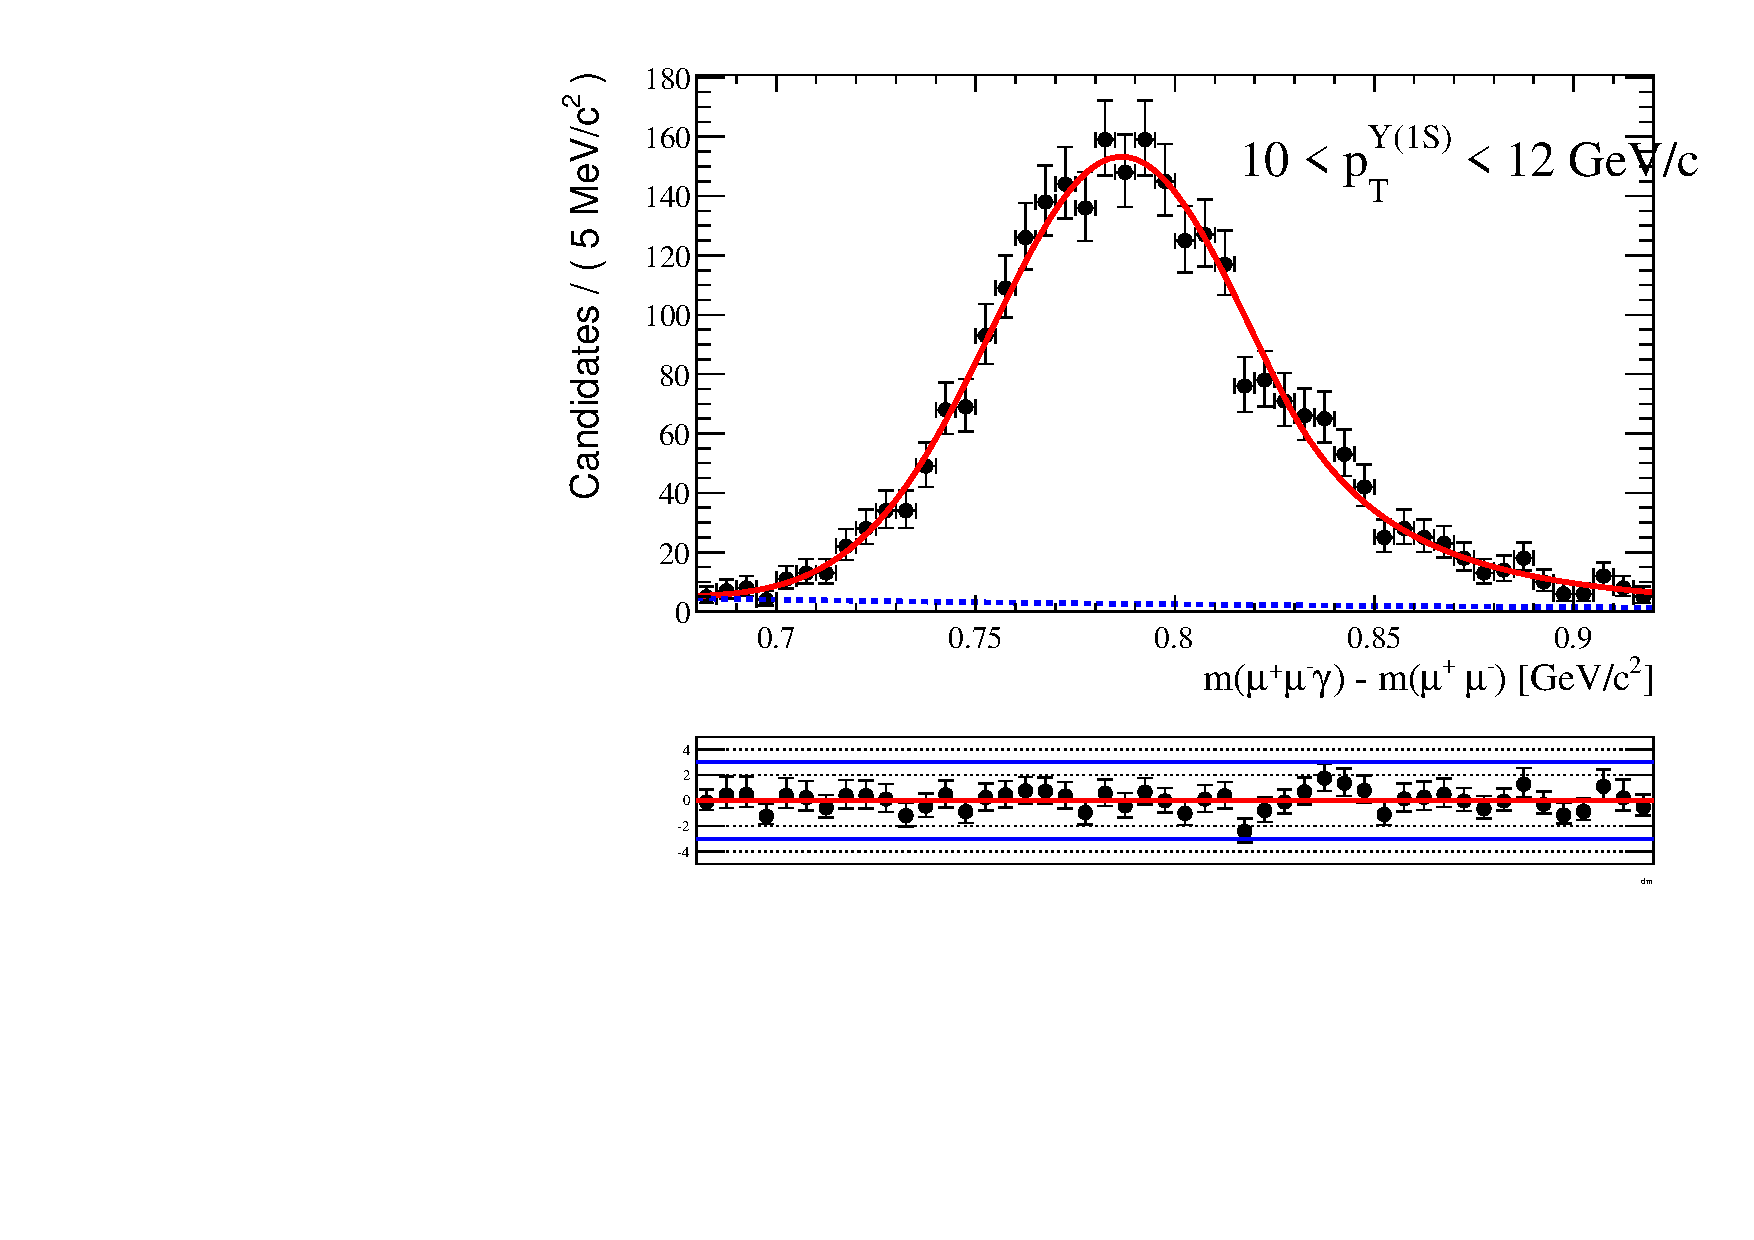
\includegraphics[width=0.16\linewidth]{fit_mc/chib12_10_12}
      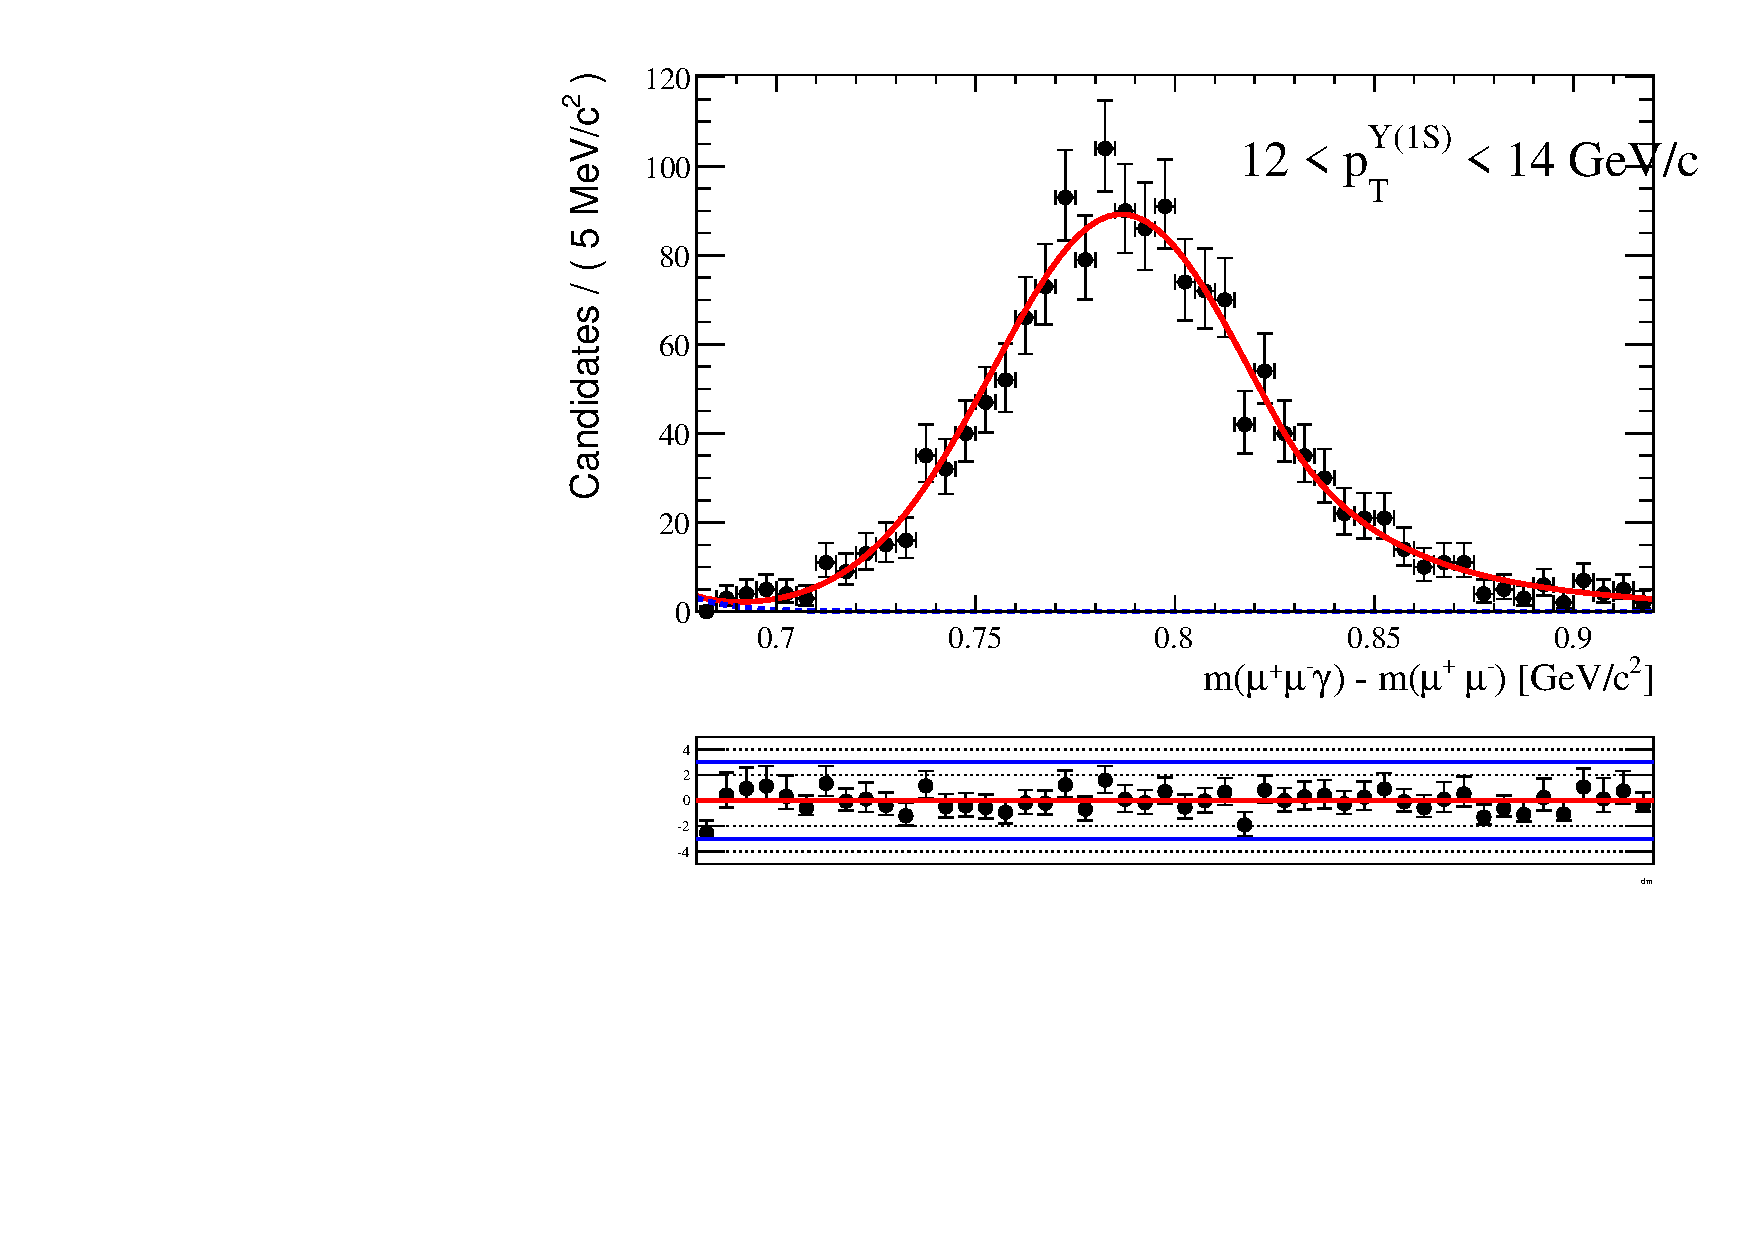
\includegraphics[width=0.16\linewidth]{fit_mc/chib12_12_14}
      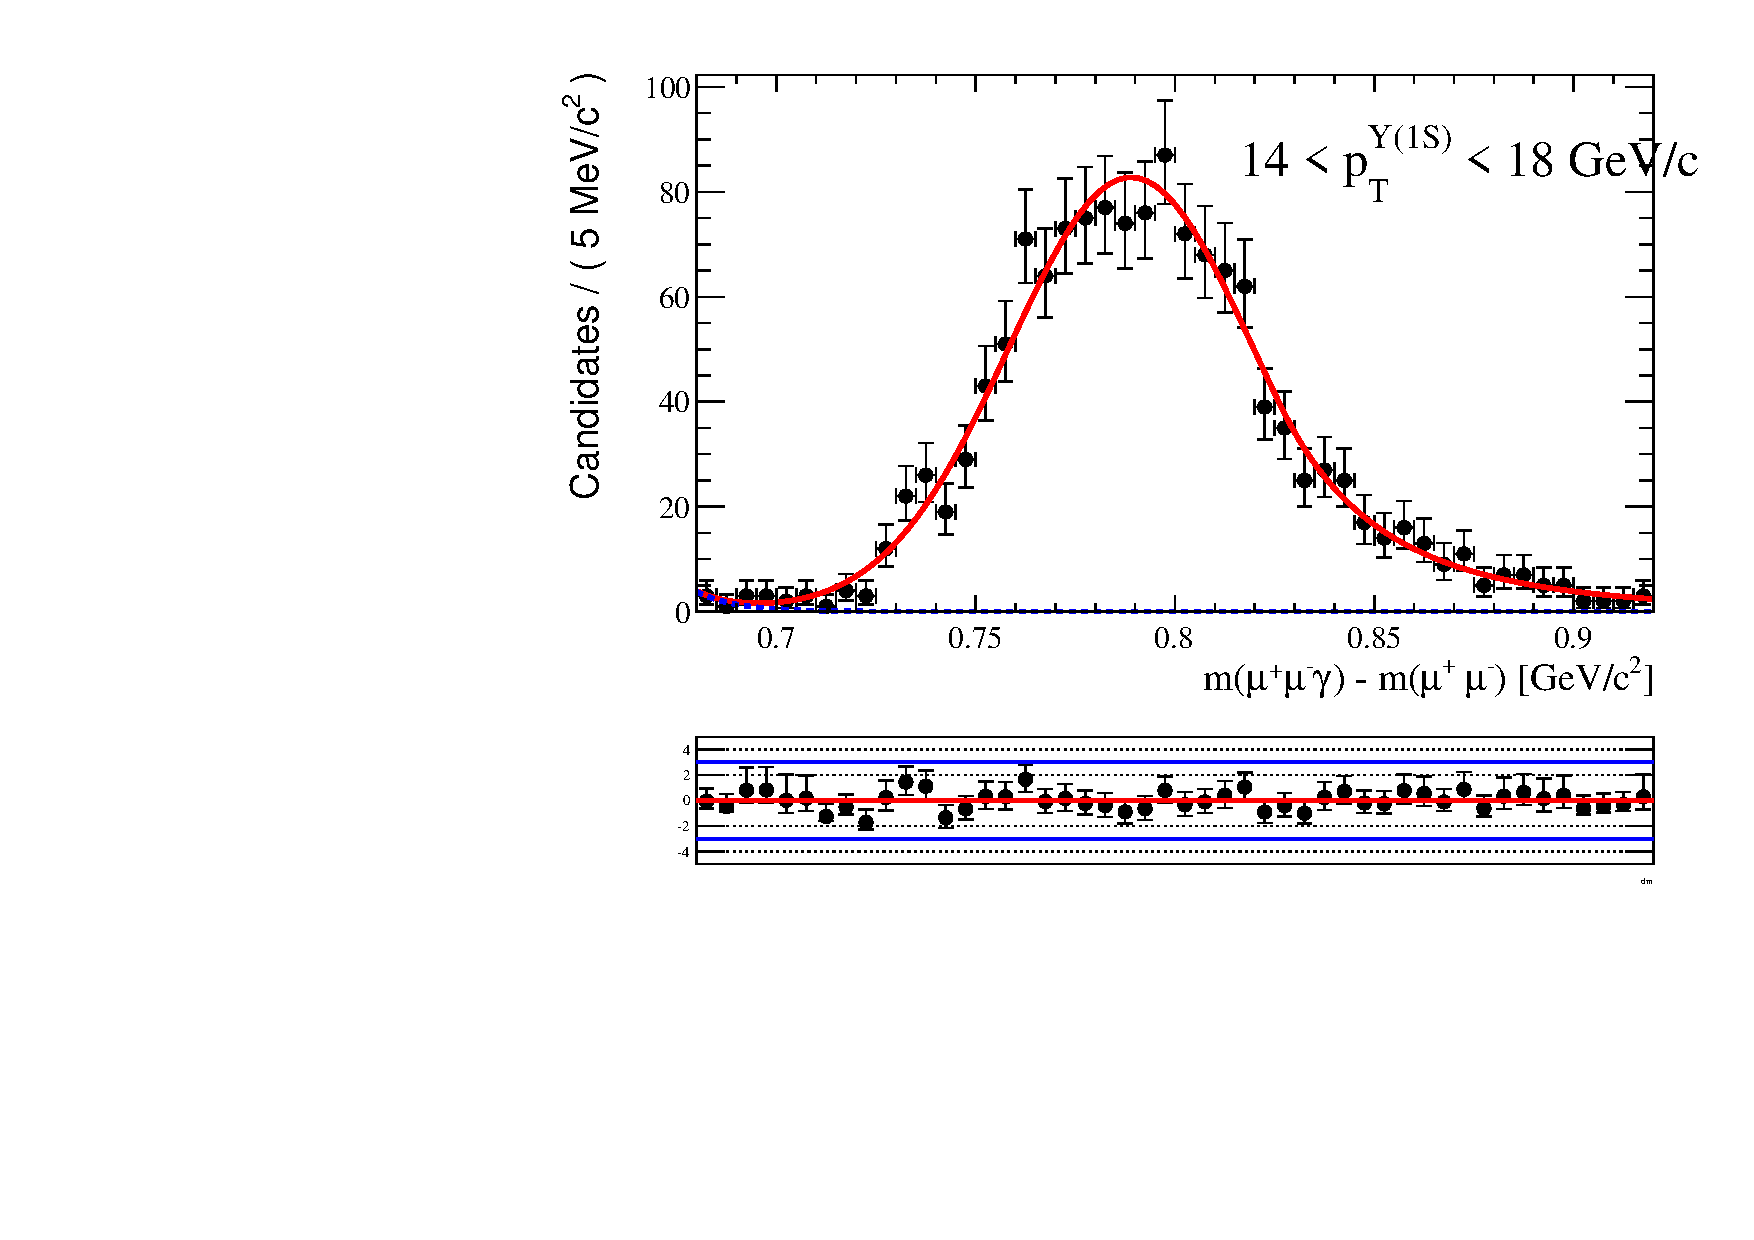
\includegraphics[width=0.16\linewidth]{fit_mc/chib12_14_18}
      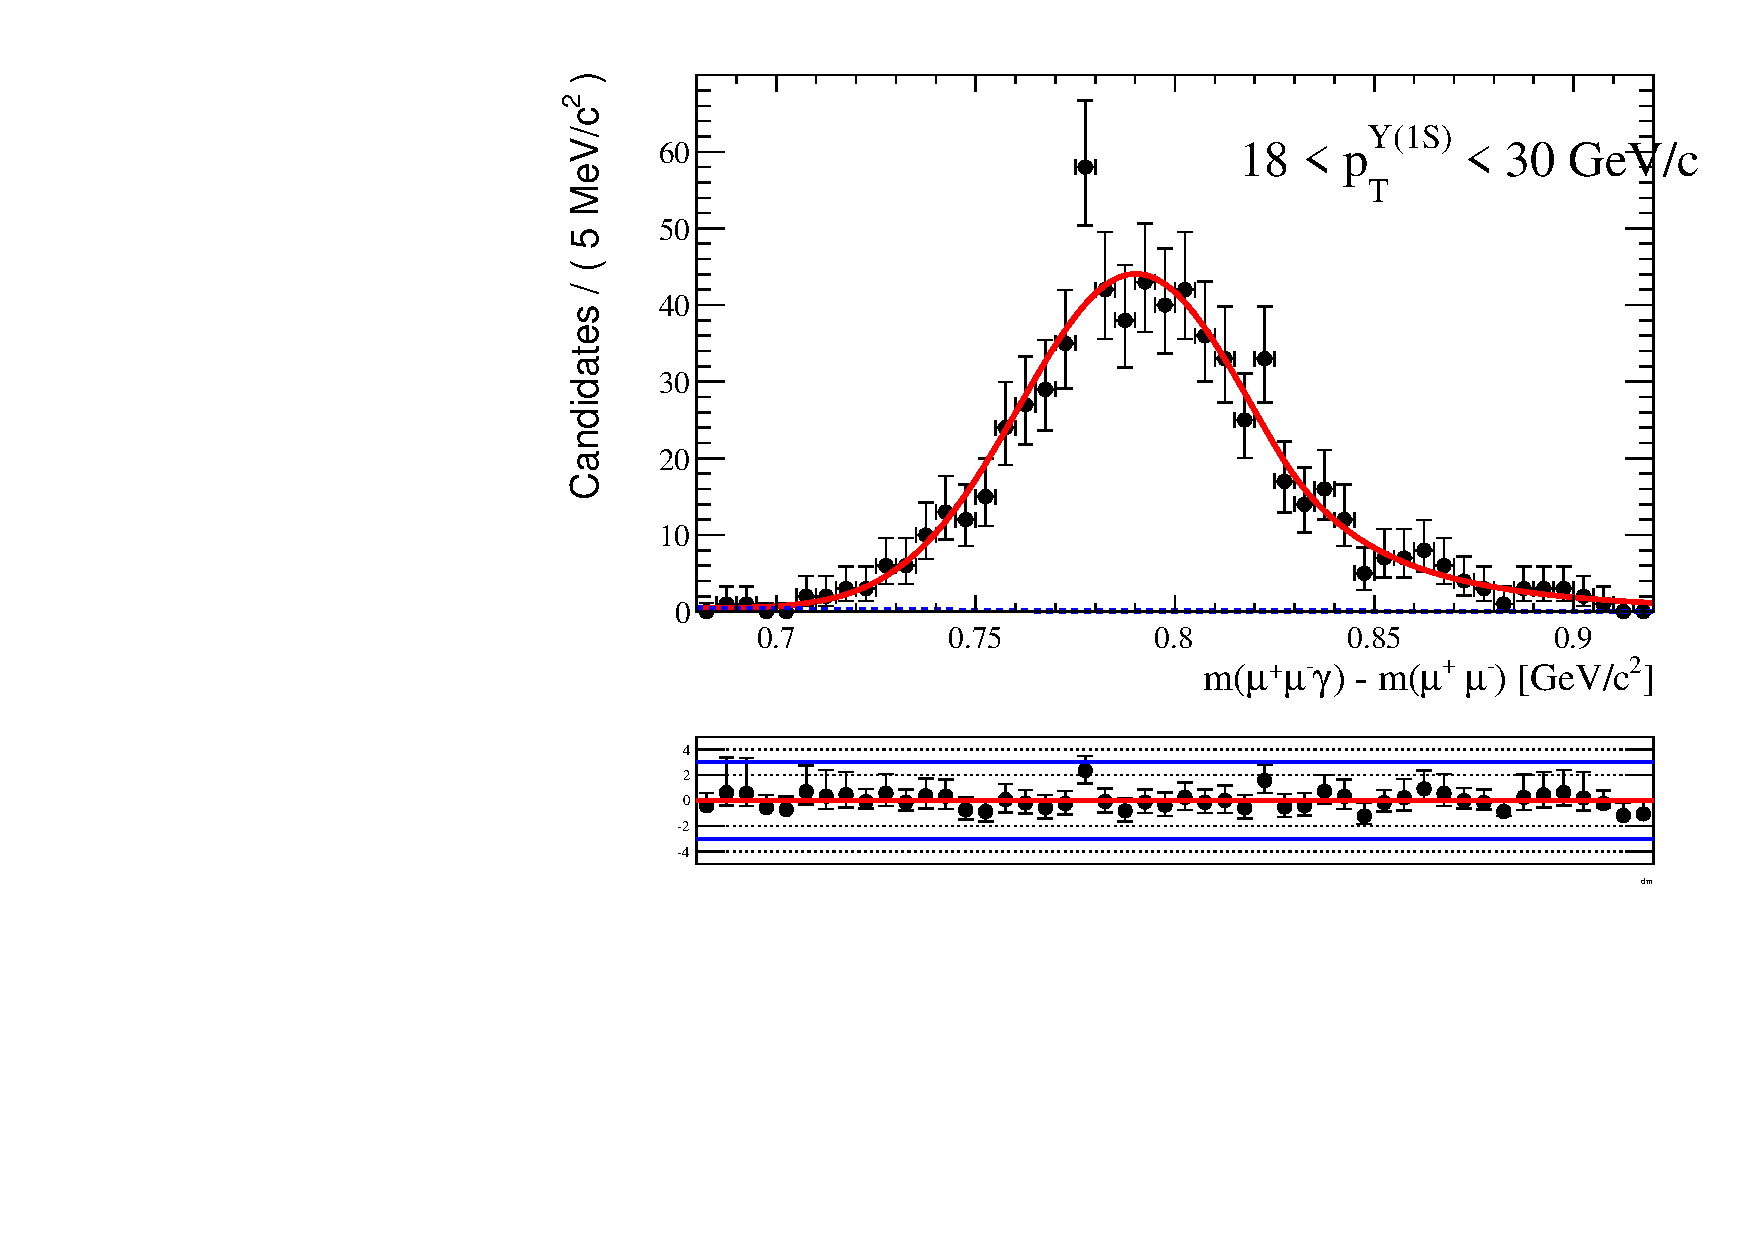
\includegraphics[width=0.16\linewidth]{fit_mc/chib12_18_30}
      \caption{\chiboneTwoP}
      \label{fig:fit_mc_chiboneTwoP}
    \end{subfigure}
    \begin{subfigure}[b]{\textwidth}
      \centering
      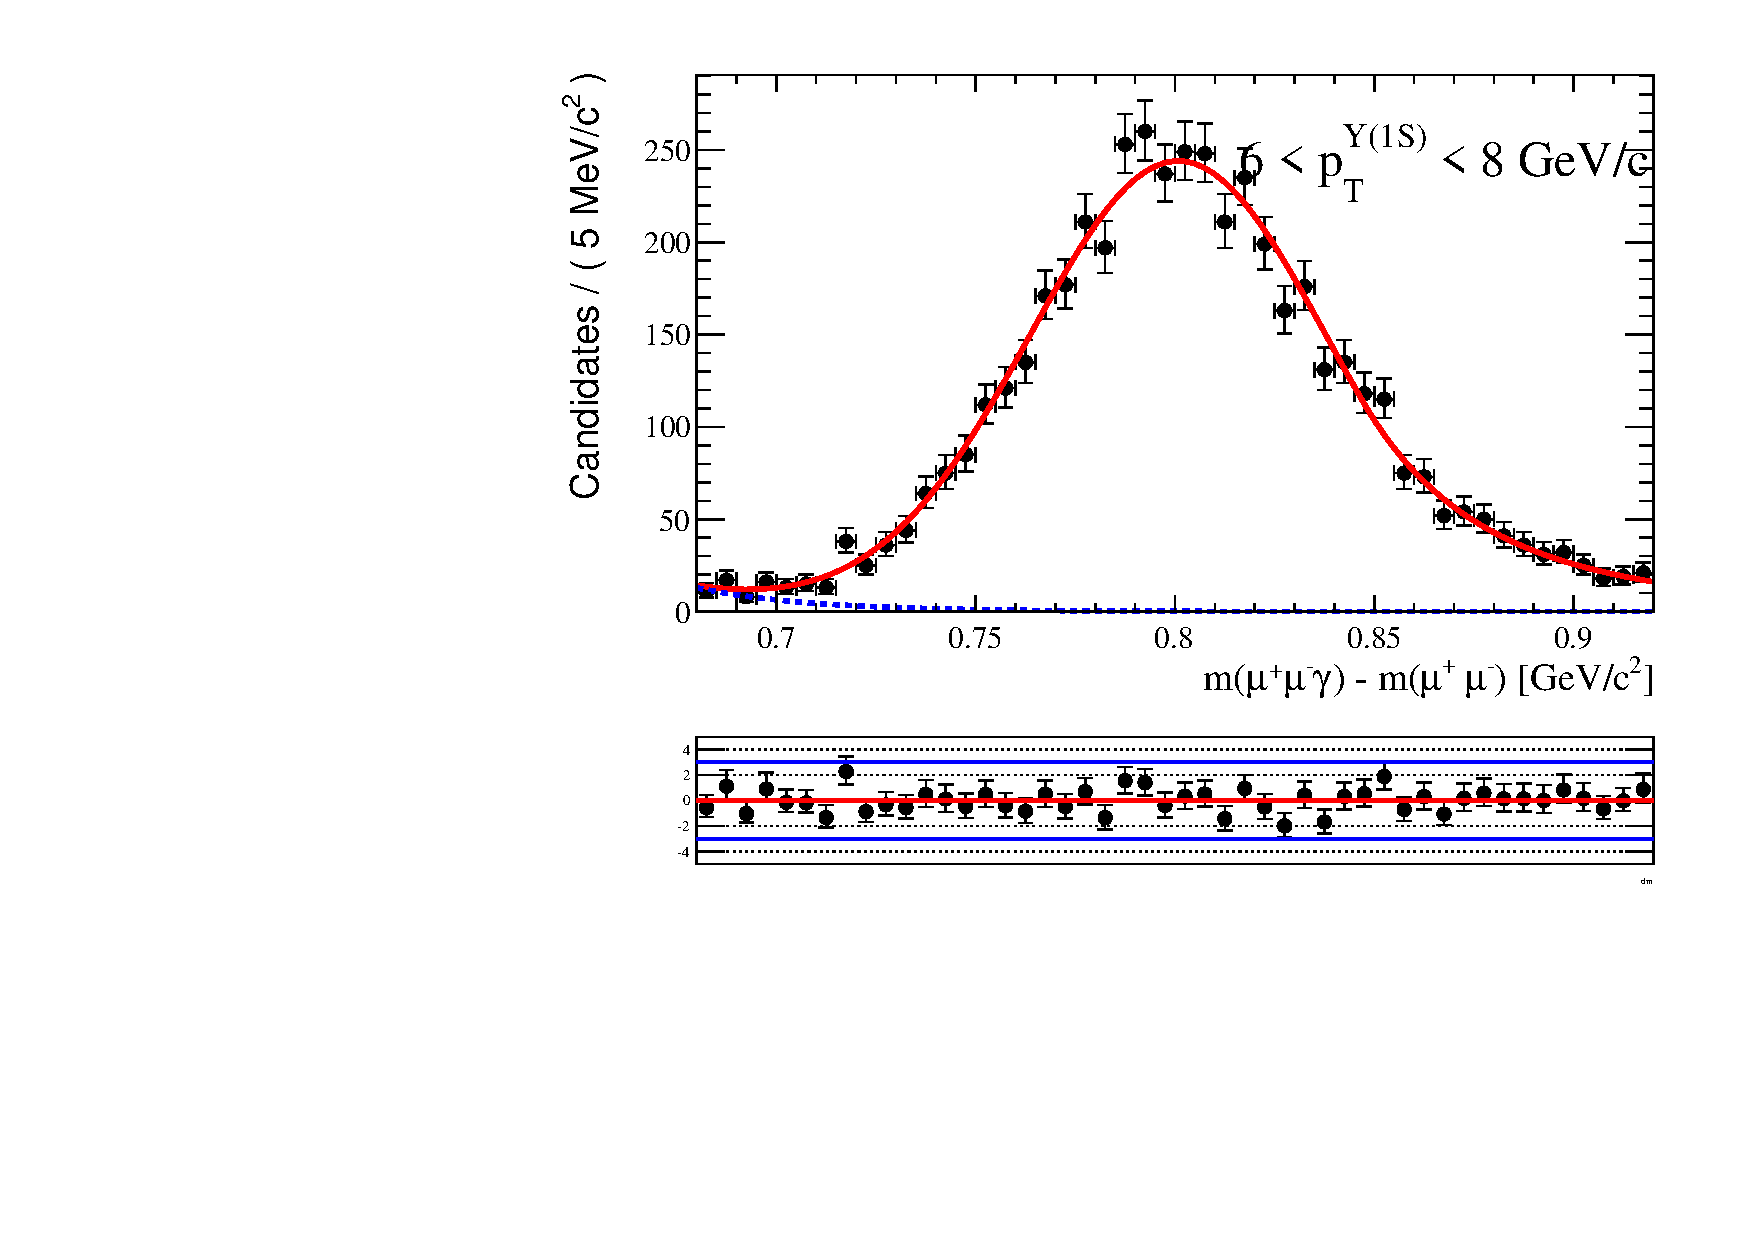
\includegraphics[width=0.16\linewidth]{fit_mc/chib22_6_8}
      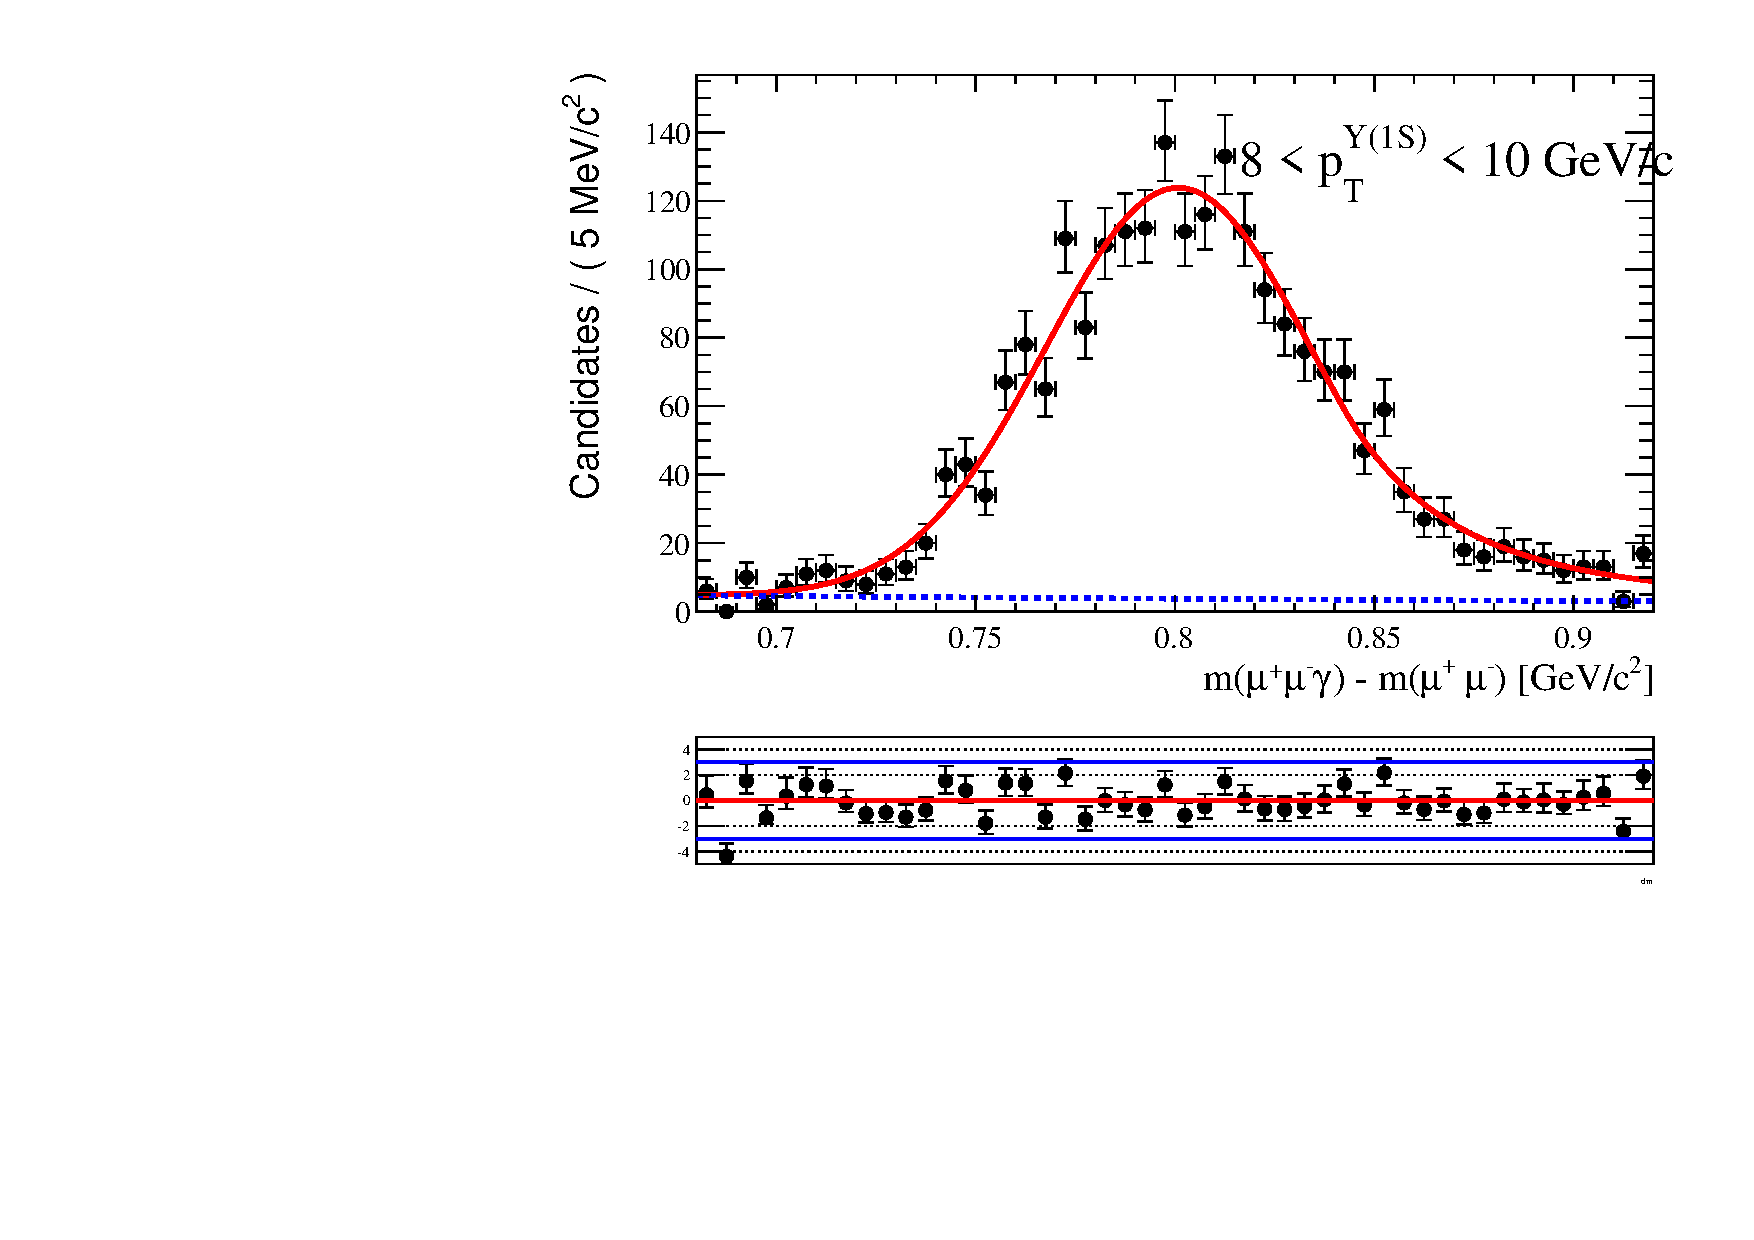
\includegraphics[width=0.16\linewidth]{fit_mc/chib22_8_10}
      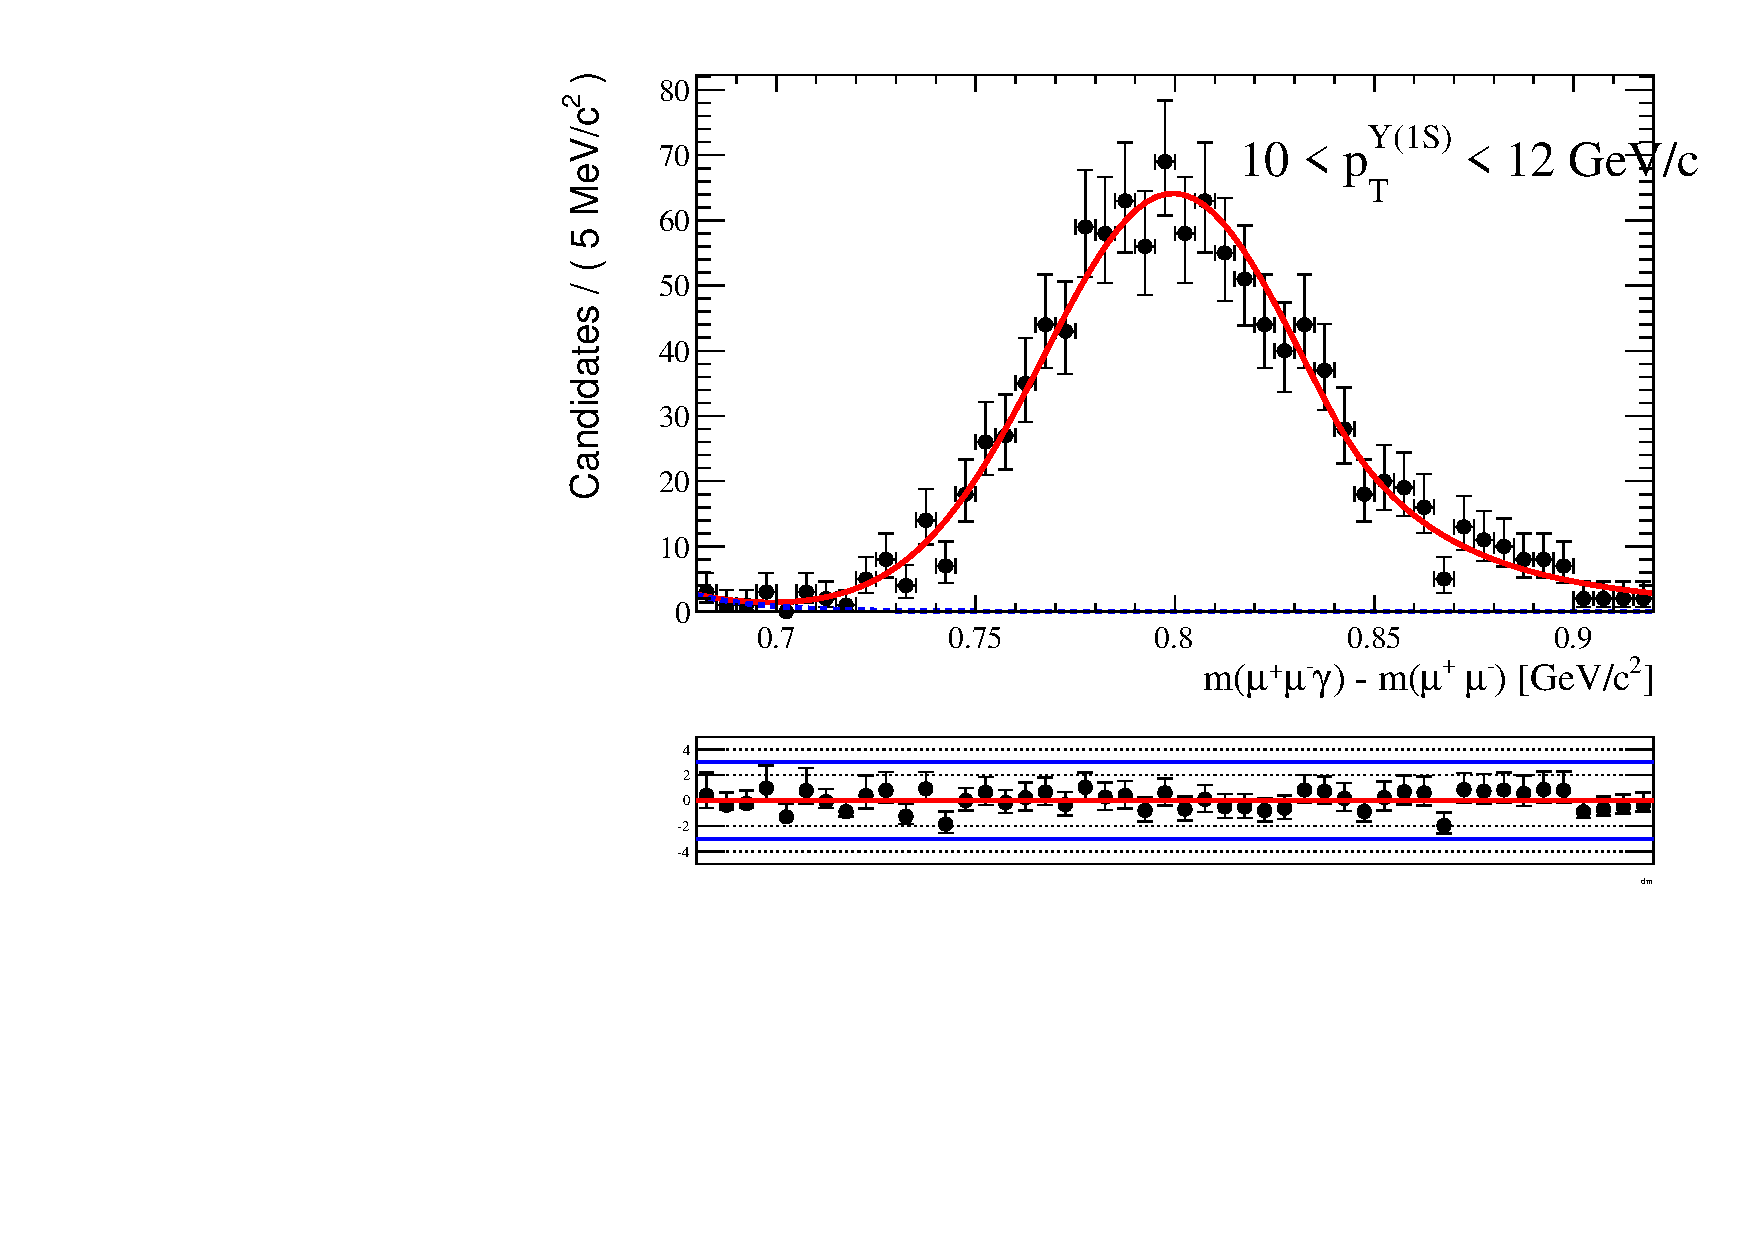
\includegraphics[width=0.16\linewidth]{fit_mc/chib22_10_12}
      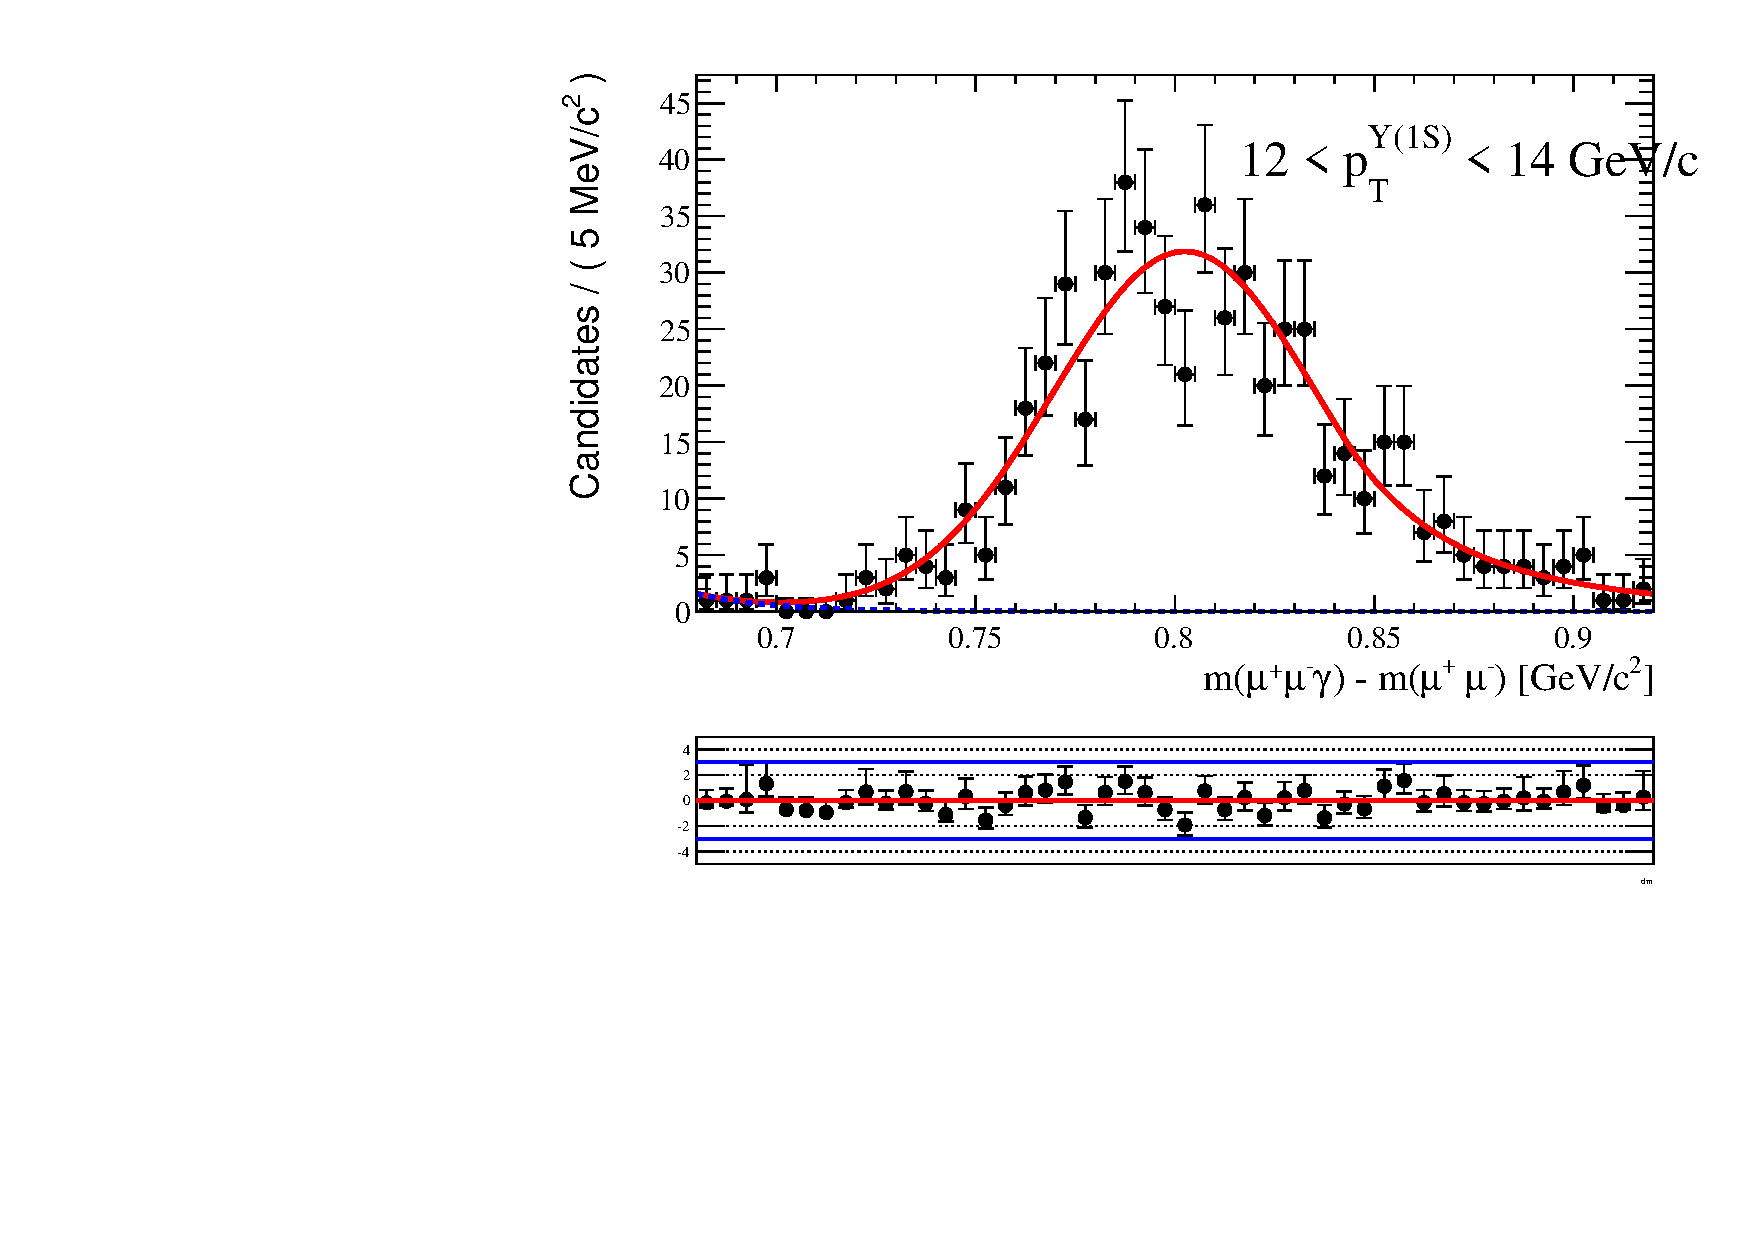
\includegraphics[width=0.16\linewidth]{fit_mc/chib22_12_14}
      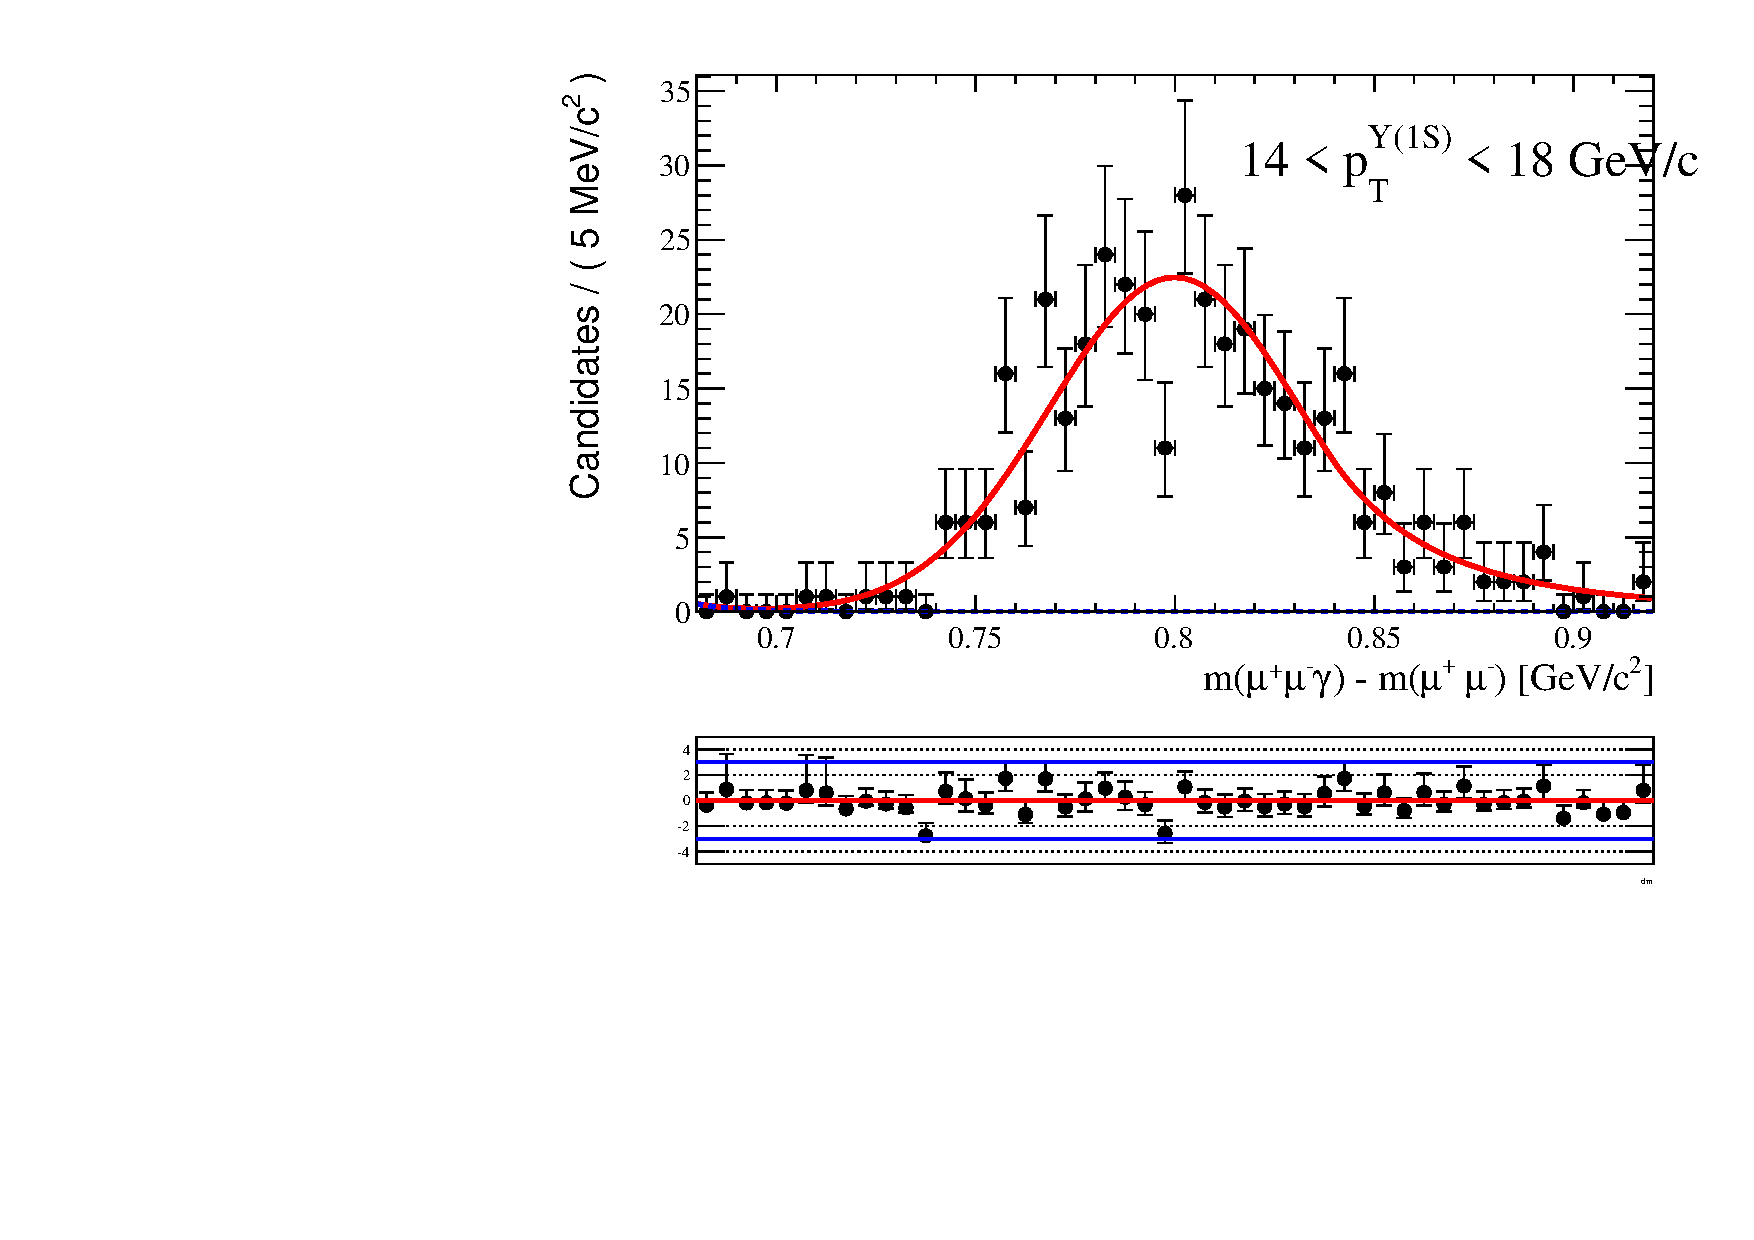
\includegraphics[width=0.16\linewidth]{fit_mc/chib22_14_18}
      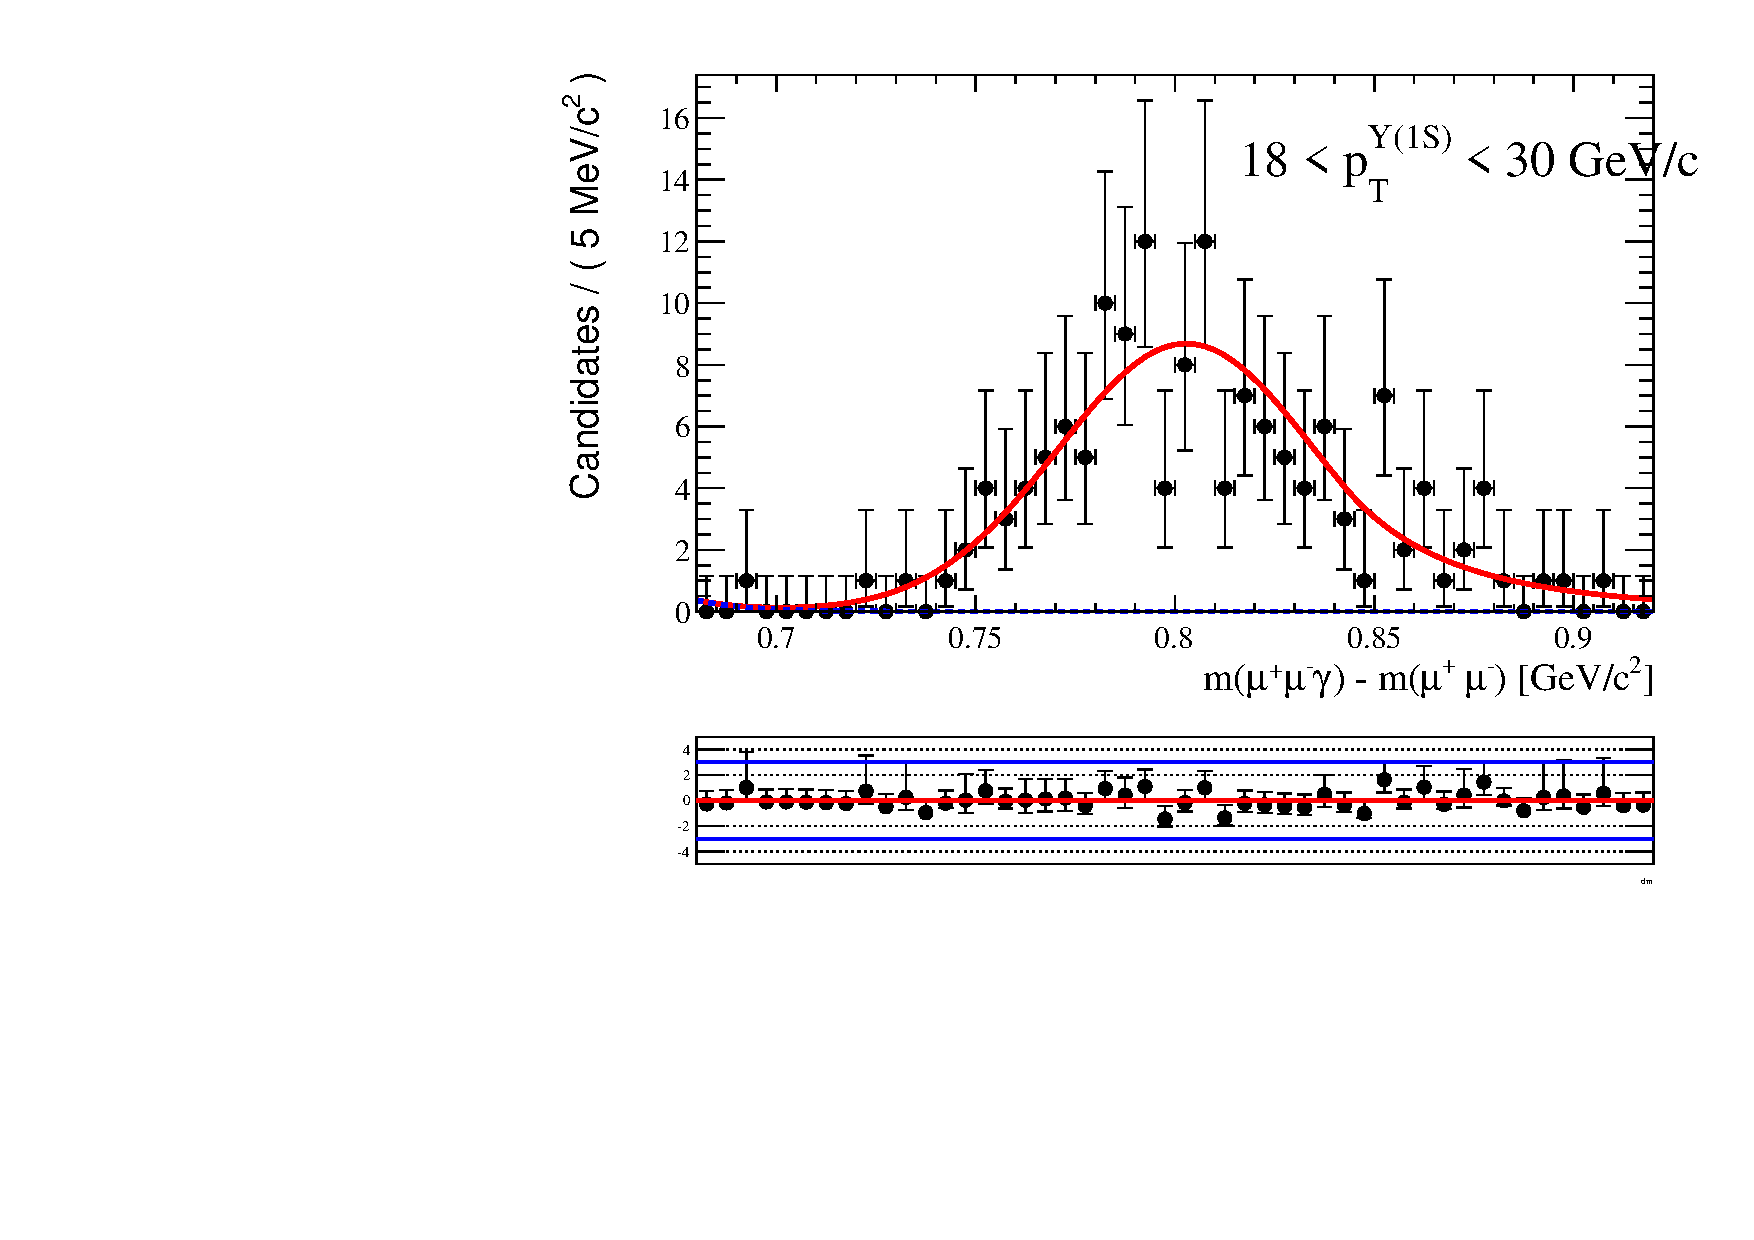
\includegraphics[width=0.16\linewidth]{fit_mc/chib22_18_30}
      \caption{\chibtwoTwoP}
      \label{fig:fit_mc_chibtwoTwoP}
    \end{subfigure}    
    \begin{subfigure}[b]{\textwidth}
      \centering
      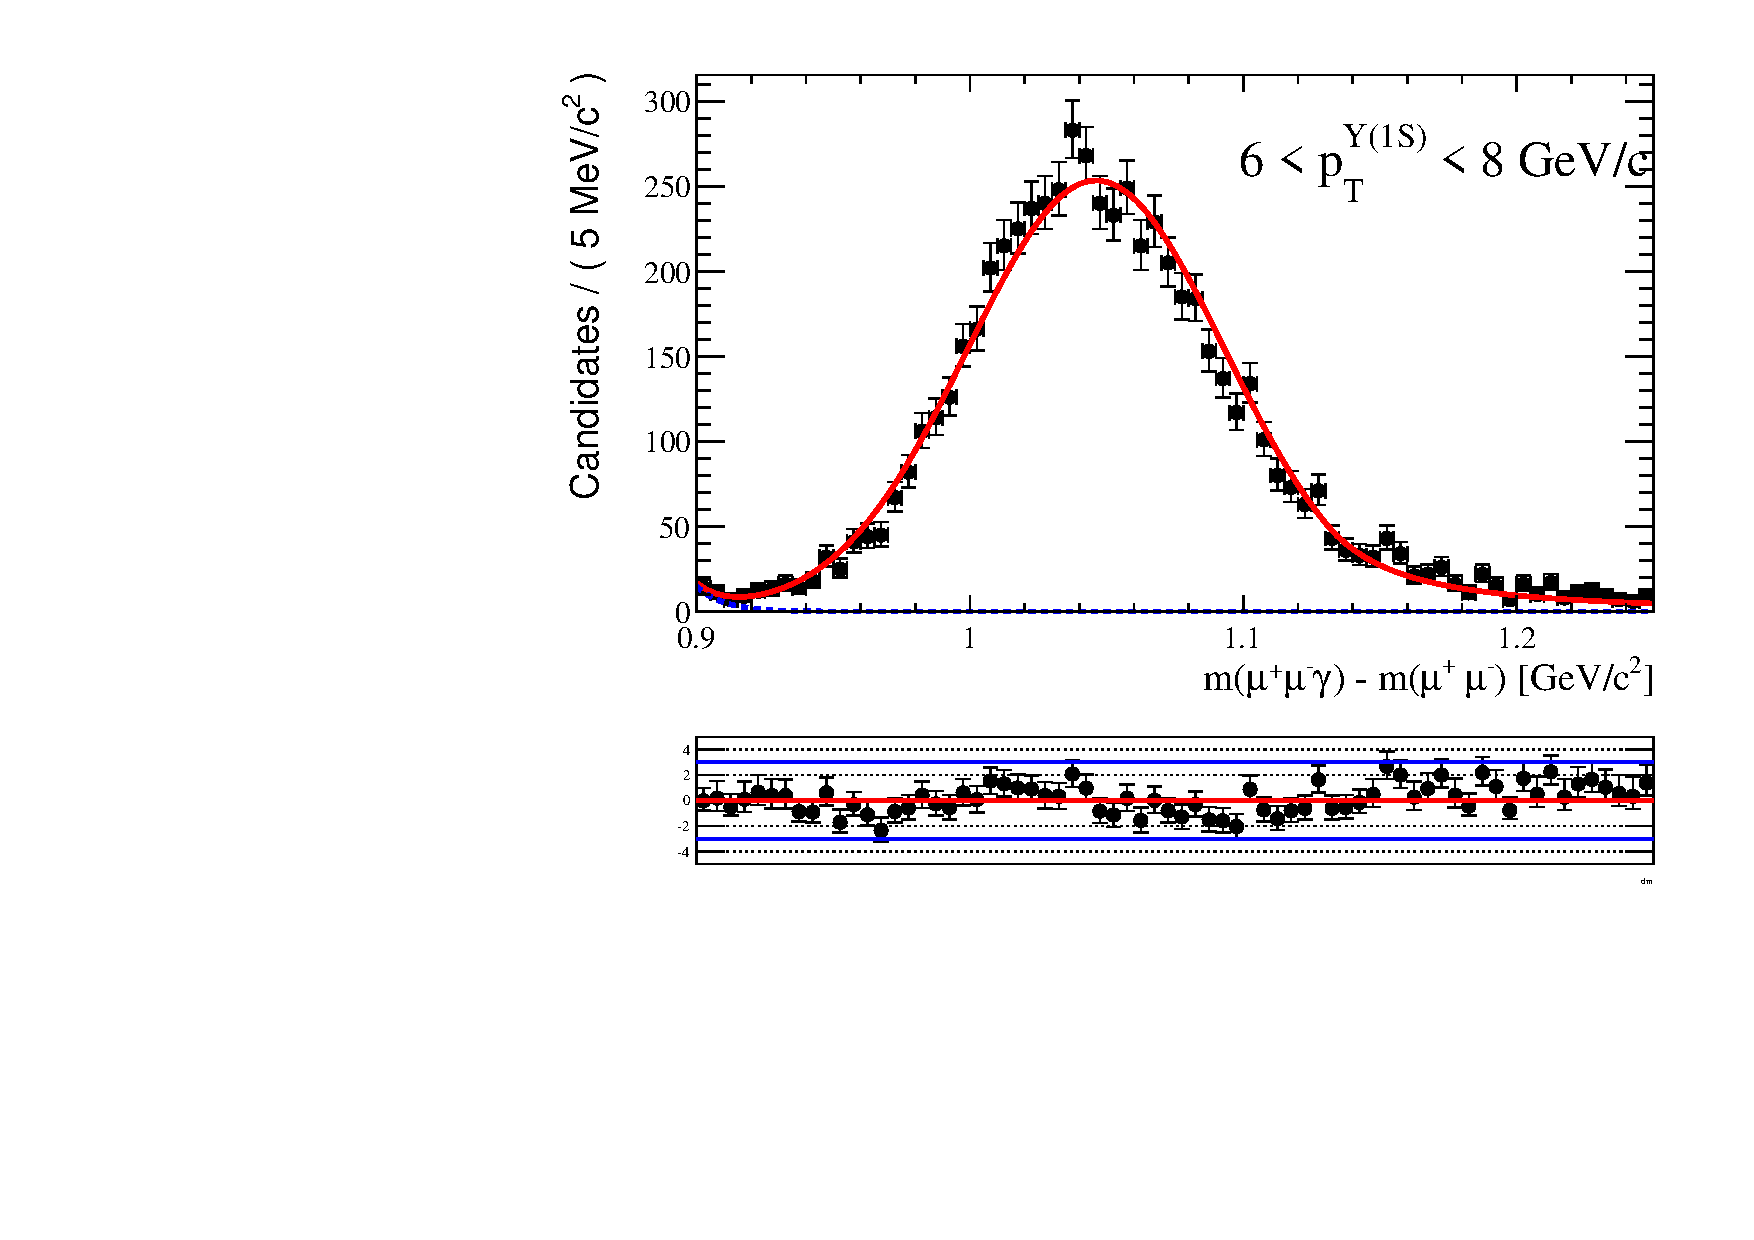
\includegraphics[width=0.16\linewidth]{fit_mc/chib13_6_8}
      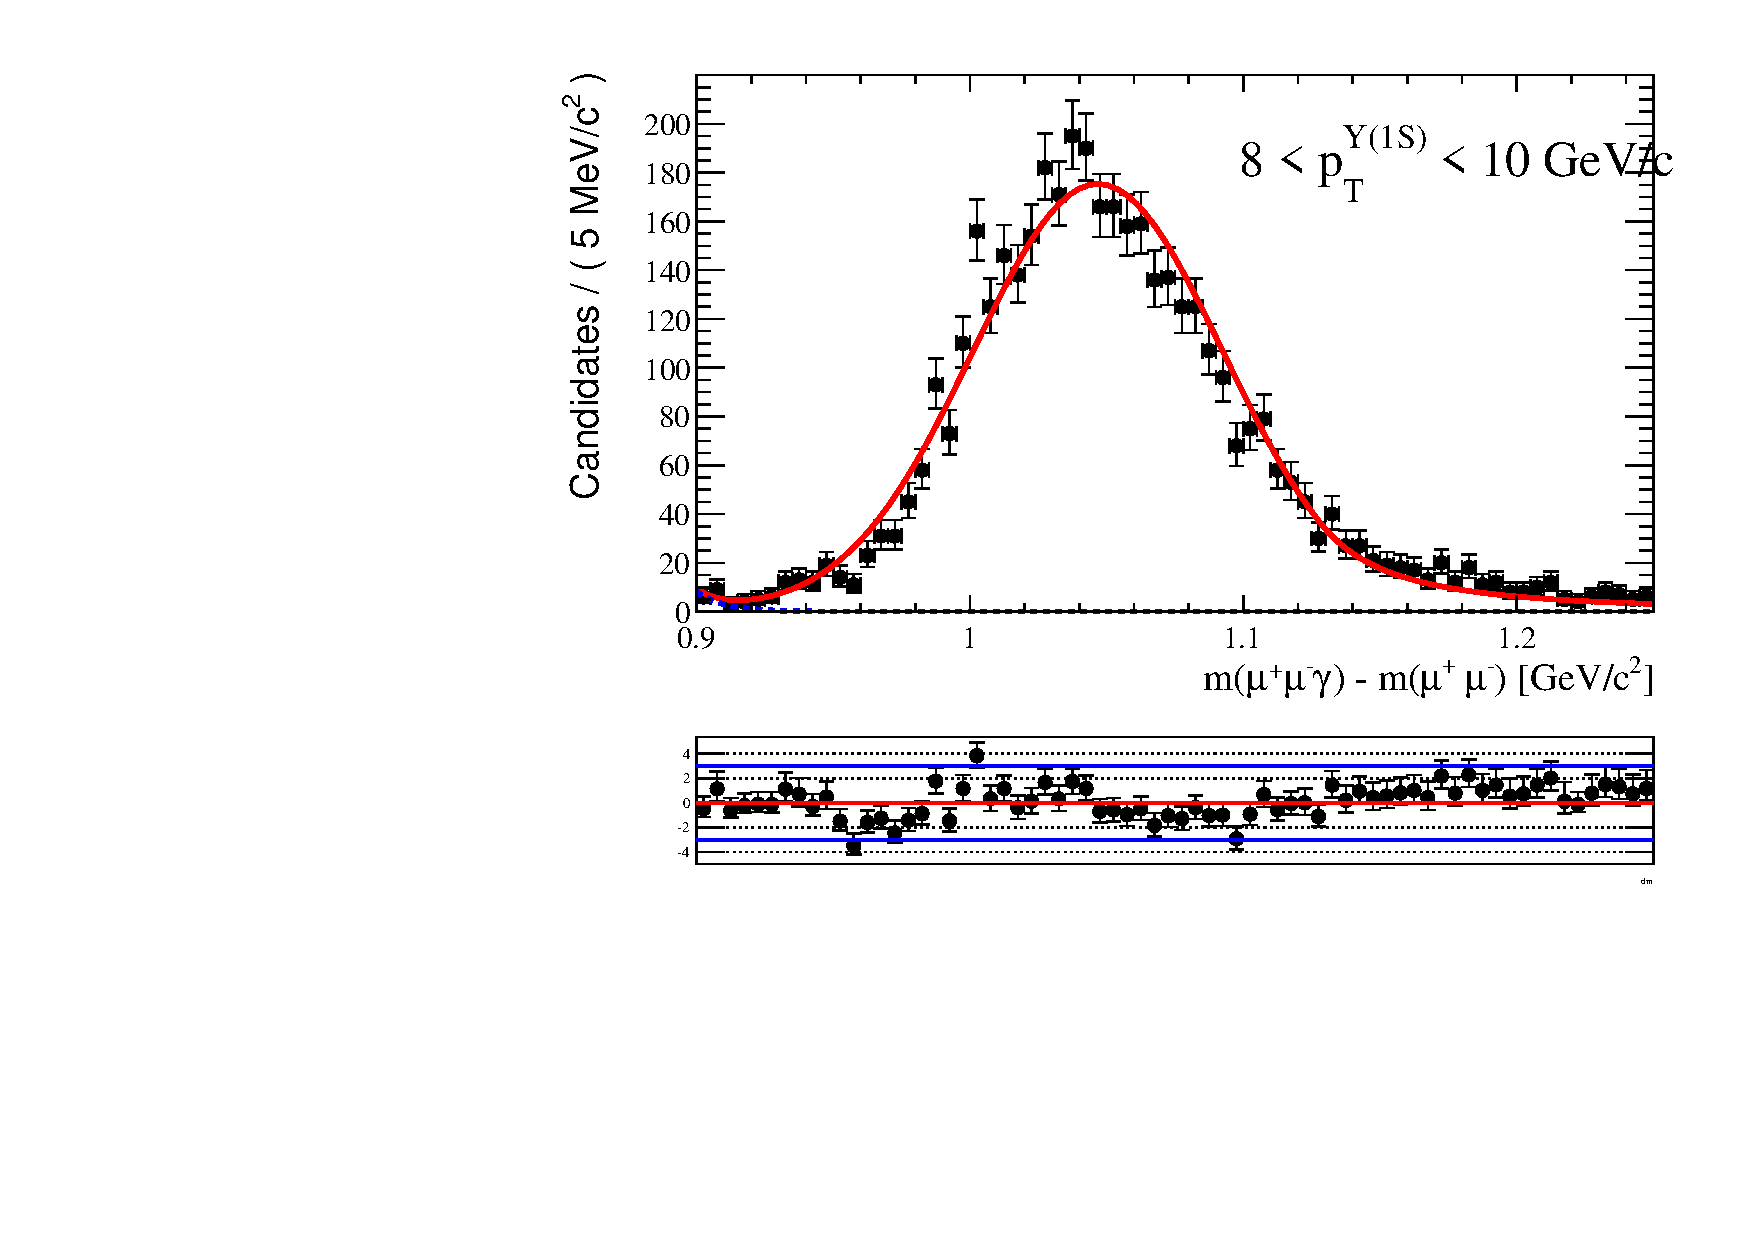
\includegraphics[width=0.16\linewidth]{fit_mc/chib13_8_10}
      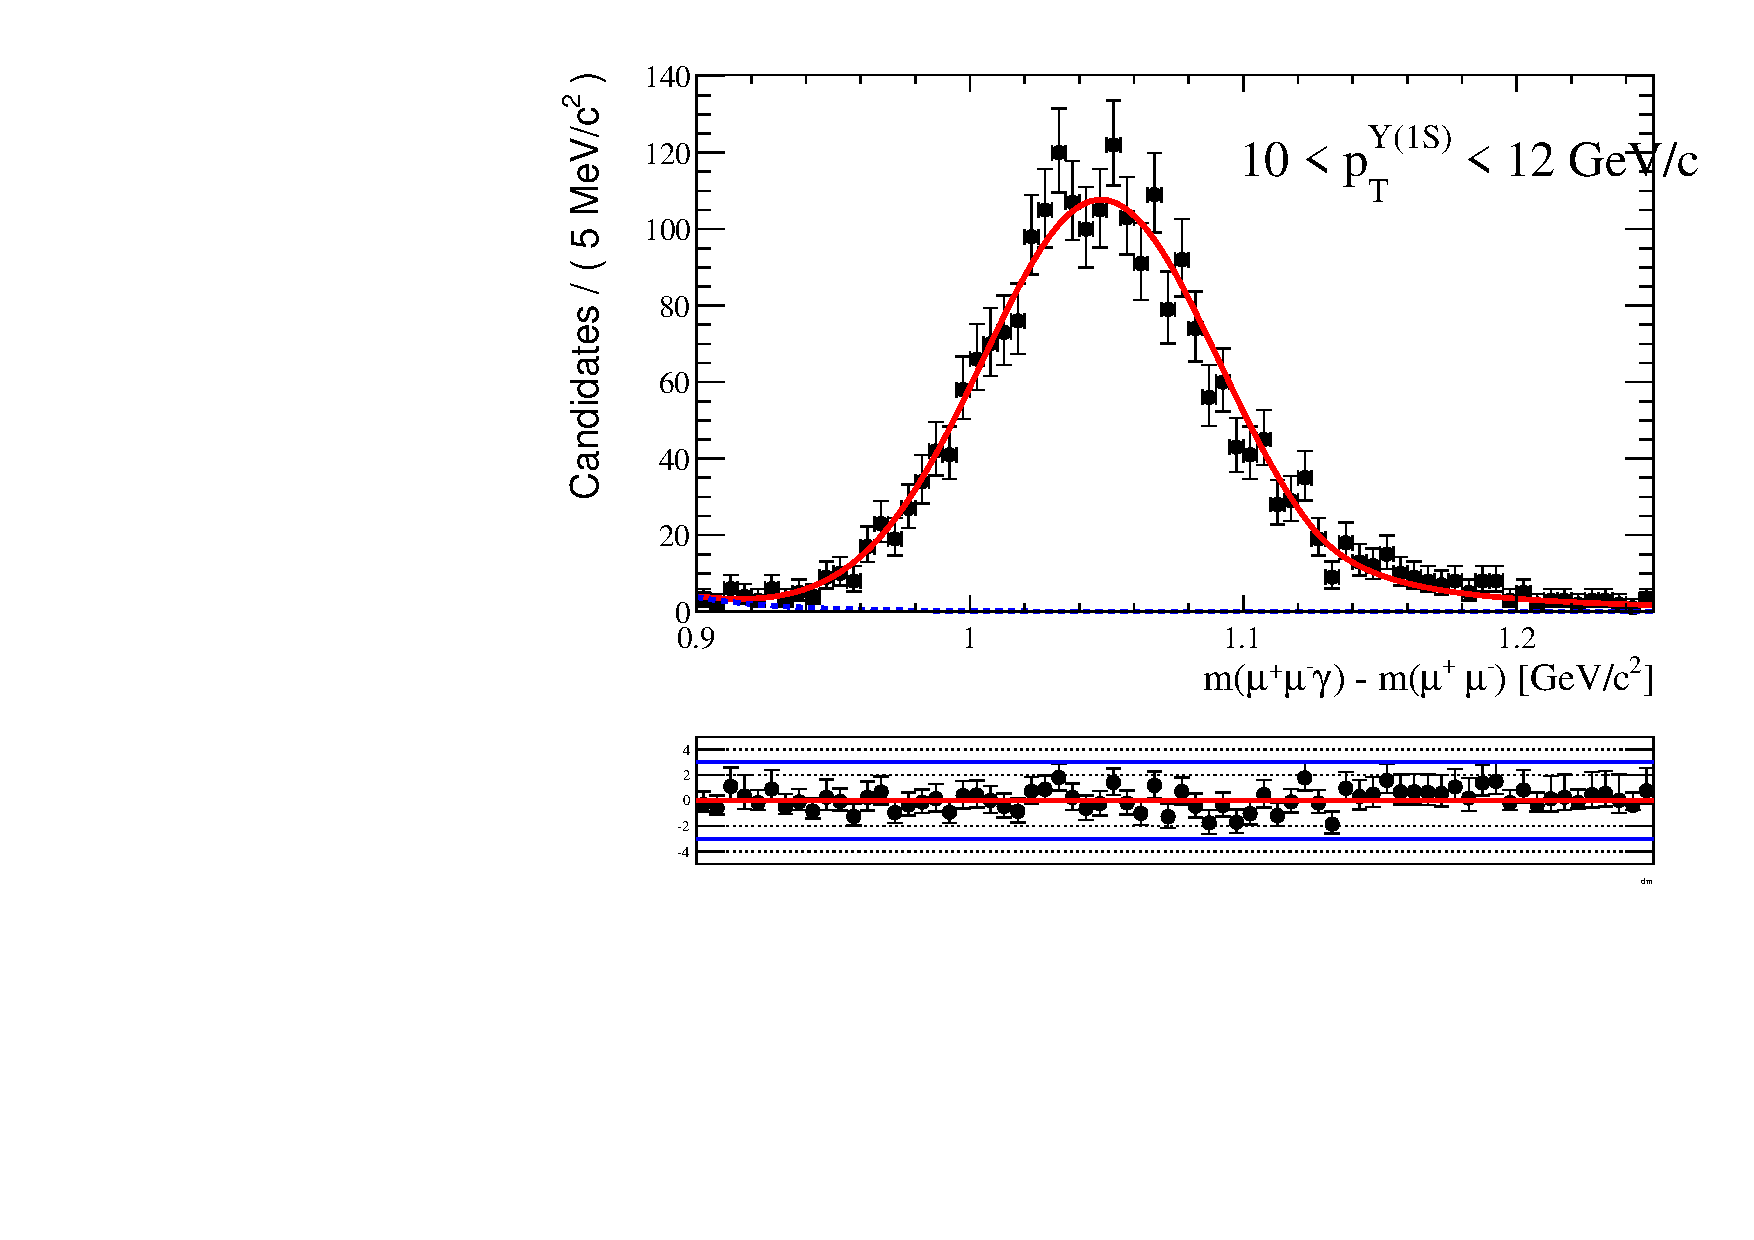
\includegraphics[width=0.16\linewidth]{fit_mc/chib13_10_12}
      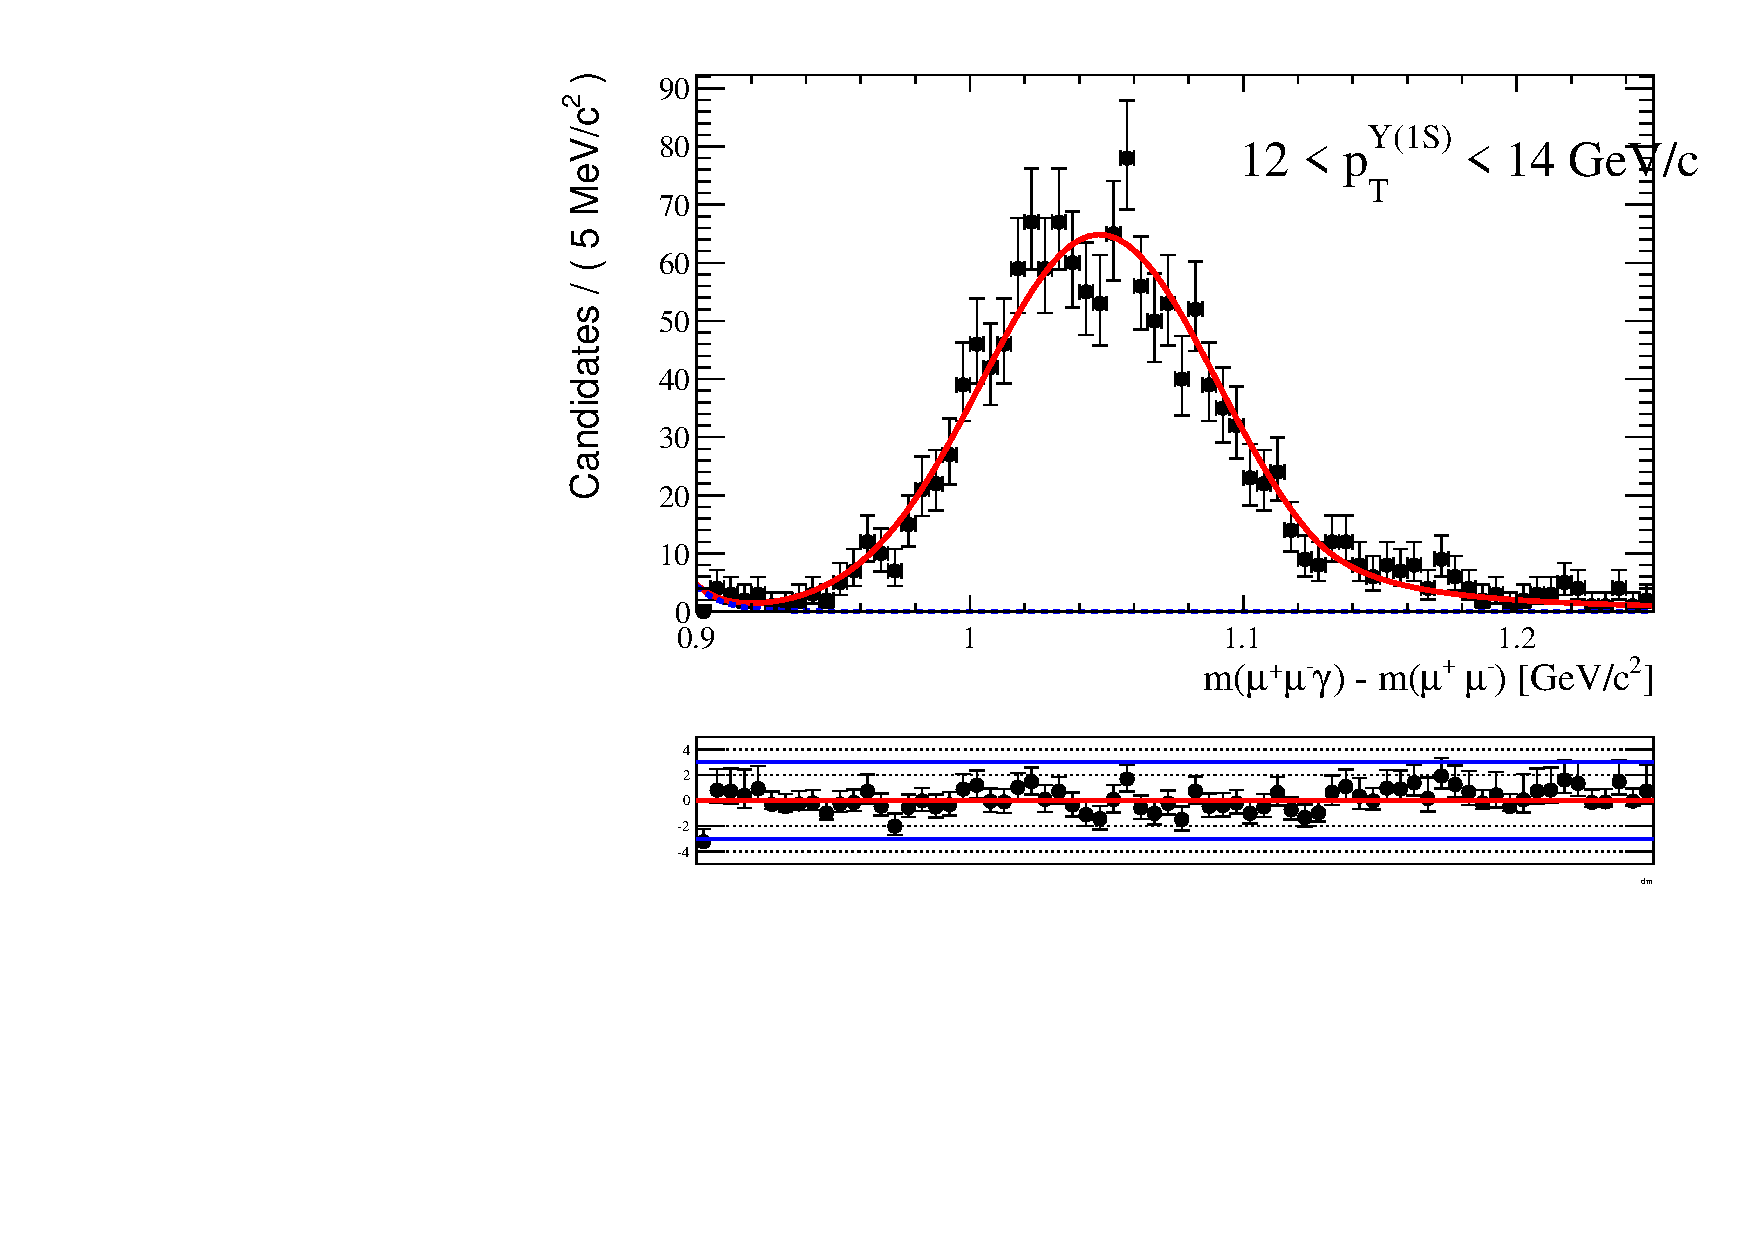
\includegraphics[width=0.16\linewidth]{fit_mc/chib13_12_14}
      \includegraphics[width=0.16\linewidth]{fit_mc/chib13_14_18}
      \includegraphics[width=0.16\linewidth]{fit_mc/chib13_18_30}
      \caption{\chiboneThreeP}
      \label{fig:fit_mc_chiboneThreeP}
    \end{subfigure}
    \begin{subfigure}[b]{\textwidth}
      \centering
      \includegraphics[width=0.16\linewidth]{fit_mc/chib23_6_8}
      \includegraphics[width=0.16\linewidth]{fit_mc/chib23_8_10}
      \includegraphics[width=0.16\linewidth]{fit_mc/chib23_10_12}
      \includegraphics[width=0.16\linewidth]{fit_mc/chib23_12_14}
      \includegraphics[width=0.16\linewidth]{fit_mc/chib23_14_18}
      \includegraphics[width=0.16\linewidth]{fit_mc/chib23_18_30}
      \caption{\chibtwoThreeP}
      \label{fig:fit_mc_chibtwoThreeP}
    \end{subfigure}        
  \caption{
    \small  Mass difference of the $\mumu \gamma$ system and $\mumu$ system for the 
    Monte Carlo data for specified interval of transverse momentum of the \OneS. The red
    solid line is the result of the fit described in the text.
  }
  \label{fig:fit_mc}
\end{figure}




\setboolean{inbibliography}{true}
\bibliographystyle{LHCb}

\end{document}
